% !TEX program = xelatex
% Отчёт TGNN-Solv с основными результатами и подробными приложениями.
\documentclass[11pt]{article}
\usepackage{fontspec}
\setmainfont{Times New Roman}
\usepackage{polyglossia}
\setdefaultlanguage{russian}
\setotherlanguage{english}
\newfontfamily\cyrillicfonttt{Andale Mono}
\usepackage[margin=1in]{geometry}
\usepackage{amsmath,amssymb,amsthm,mathtools}
\usepackage{booktabs,longtable,tabularx,array,multirow}
\usepackage{graphicx}
\usepackage{caption}
\usepackage{float}
\usepackage{flafter}
\usepackage[section]{placeins}
\usepackage{xcolor}
\usepackage{hyperref}
\usepackage{alphalph}
\usepackage{microtype}
\usepackage{etoolbox}
\usepackage{needspace}
\setlength{\emergencystretch}{2em}
\definecolor{ReportBlue}{HTML}{315F72}
\hypersetup{colorlinks=true,linkcolor=black,urlcolor=ReportBlue,citecolor=black}
\graphicspath{{figures/}}

\newcolumntype{Y}{>{\raggedright\arraybackslash}X}
\newcolumntype{C}[1]{>{\centering\arraybackslash}p{#1}}
\newcolumntype{P}[1]{>{\raggedright\arraybackslash}p{#1}}
\DeclareRobustCommand{\code}[1]{\texttt{\detokenize{#1}}}
\newcommand{\mae}{\mathrm{MAE}}
\newcommand{\rmse}{\mathrm{RMSE}}
\newcommand{\Rtwo}{R^2}
\newcommand{\dd}{\,\mathrm{d}}
\newcommand{\E}{\mathbb{E}}
\newcommand{\Var}{\mathrm{Var}}
\newcommand{\Cov}{\mathrm{Cov}}
\newcommand{\abs}[1]{\left\lvert #1 \right\rvert}
\newcommand{\norm}[1]{\left\lVert #1 \right\rVert}
\newcommand{\lnx}{\ln x_2}
\newcommand{\lngamma}{\ln \gamma_2}
\newcommand{\Tm}{T_{\mathrm m}}
\newcommand{\Rgas}{R}
\newcommand{\dHfus}{\Delta H_{\mathrm{fus}}}
\newcommand{\dGfus}{\Delta G_{\mathrm{fus}}}
\newcommand{\dCpfus}{\Delta C_p^{\mathrm{fus}}}
\newcommand{\dSfus}{\Delta S_{\mathrm{fus}}}
\newcommand{\gammainf}{\gamma_2^{\infty}}

\theoremstyle{definition}
\newtheorem{definition}{Определение}[section]
\newtheorem{estimate}{Оценка}[section]
\newtheorem{claim}{Утверждение}[section]
\newtheorem{remark}{Замечание}[section]

\setlength{\parindent}{0pt}
\setlength{\parskip}{0.58\baselineskip}
\setlength{\tabcolsep}{4.5pt}
\renewcommand{\arraystretch}{1.16}
\captionsetup[figure]{font=small,labelfont=bf,skip=6pt}
\captionsetup[table]{font=small,labelfont=bf,skip=6pt}
\setlength{\textfloatsep}{9pt plus 2pt minus 2pt}
\setlength{\floatsep}{8pt plus 2pt minus 2pt}
\setlength{\intextsep}{8pt plus 2pt minus 2pt}
\renewcommand{\topfraction}{0.94}
\renewcommand{\bottomfraction}{0.82}
\renewcommand{\textfraction}{0.06}
\renewcommand{\floatpagefraction}{0.68}
\makeatletter
\renewcommand*\l@section{\@dottedtocline{1}{1.5em}{3.2em}}
\renewcommand*\l@subsection{\@dottedtocline{2}{4.7em}{4.0em}}
\setlength{\@fptop}{0pt}
\setlength{\@fpsep}{8pt plus 1fil}
\setlength{\@fpbot}{0pt plus 1fil}
\makeatother
\preto\section{\Needspace{11\baselineskip}}
\preto\subsection{\Needspace{8\baselineskip}}
\emergencystretch=3em
\frenchspacing


\title{TGNN-Solv\\
\large Физически информированная графовая модель для предсказания растворимости}
\author{Поломошнов Никита Львович}
\date{25 апреля 2026 г.}

\begin{document}
\sloppy
\raggedbottom
\maketitle
\newpage

\section*{Резюме для руководителя}
\addcontentsline{toc}{section}{Резюме для руководителя}

Главный поддерживаемый результат по основному разбиению по новым каркасам пока остаётся отрицательным: на нём TGNN-Solv даёт $\mae=1.741$, DirectGNN --- $\mae=1.652$, а случайный лес с гибридными признаками --- $\mae=1.722$. Но новая внутренняя проверка \emph{crystal-known probe}, где на всех строках известны и $\Tm$, и $\dHfus$, впервые даёт локальный выигрыш физического пути без постобработки и без внешнего оракула на тесте: TGNN-Solv имеет $\mae=0.601$, $\Rtwo=0.633$ и смещение $+0.087$, тогда как DirectGNN даёт $\mae=0.818$, $\Rtwo=0.569$ и смещение $-0.370$. Это ещё не доказательство общего превосходства TGNN-Solv, а первый количественный сигнал, что физическое узкое место может помогать, когда кристаллическая часть задачи хорошо определена.

Эта локальная победа не означает, что проблема диапазона решена. На crystal-known probe отношение $\sigma(\hat y)/\sigma(y)$ равно только $0.518$ у стандартного TGNN-Solv и $0.463$ у DirectGNN. Значит, выигрыш идёт не через восстановление полной амплитуды предсказаний, а через лучшее ранжирование и меньший bias. В этом смысле физический путь уже полезен, но пока не полностью раскрывает наблюдаемый диапазон растворимостей.

Оракульная диагностика дала более важный структурный вывод. Если в уже обученный TGNN-Solv принудительно подставить истинные $\Tm$ и $\dHfus$ на этапе применения, результат резко ухудшается: $\mae$ растёт до $1.244$, а $\sigma(\hat y)/\sigma(y)$ падает до $0.074$. Train-time oracle улучшает MAE лишь умеренно, до $0.567$, но ухудшает $\Rtwo$ до $0.512$ и увеличивает смещение до $+0.393$. Это означает, что модель выучила не независимые физические ветви, а согласованную компенсацию между $\Phi(T)$ и $\ln\gamma_2$.

Количественная проверка этой компенсации подтверждает вывод прямо на строках crystal-known probe. Для стандартного TGNN-Solv ошибки $\delta\Phi=\Phi_{\mathrm{pred}}-\Phi_{\mathrm{true}}$ и $\delta\gamma=\ln\gamma_{2,\mathrm{pred}}-\ln\gamma_{2,\mathrm{req}}$ имеют противоположный знак на всех $8$ тестовых строках, их корреляция равна $-0.876$, а среднее $\abs{\delta\Phi+\delta\gamma}$ равно $0.590$. После forced-oracle eval кристаллическая ошибка почти исчезает ($\delta\Phi\approx0$), но среднее $\abs{\delta\Phi+\delta\gamma}$ вырастает до $1.242$: компенсация ломается, и ошибка резко растёт. Это не баг решателя, а типичная coupled decomposition для физически информированной модели с двумя совместно обучаемыми вкладами.

Прямая малая абляция этого механизма через опциональный штраф декорреляции пока не дала качественного размыкания. На том же crystal-known probe sweep весов $L_{\mathrm{decorr}}$ от $0.05$ до $0.50$ слегка улучшил стандартный test-MAE только до $0.597$ и поднял отношение $\sigma(\hat y)/\sigma(y)$ лишь до $0.525$, но корреляция $\delta\Phi$ и $\delta\gamma$ осталась практически неизменной (около $-0.876$), а forced-oracle MAE осталась около $1.242$. Значит, на текущем микросрезе этот член функции ошибки действует скорее как слабая регуляризация, а не как решение проблемы идентифицируемости.

Это отрицательное наблюдение теперь поддержано и с внешней стороны данных. По локальному ThermoML-кэшу собран уже не только конечноконцентрационный activity-контур, но и exact-pair coverage audit по всем бинарным ThermoML property-лейблам, а также measurement-level harvest по совпавшим парам. Он показывает, что общее pair-level пересечение с SLE-корпусом вовсе не нулевое: найдено $2353$ exact SLE pair overlap из $12129$ поддерживаемых пар, то есть примерно $19$--$21\%$ по train/val/test, с $454$ DOI и $30336$ агрегированных exact-state измерений. Однако почти весь этот overlap относится к composition-like и общим физическим свойствам, а не к branch-specific сигналу на активность. Если оставить только candidate family для activity-ветви --- direct activity, solution thermodynamics, excess mixing enthalpy и VLE-like свойства --- property-level покрытие схлопывается до $14$ train-пар, $0$ val-пар и $2$ test-пар, а measurement-backed usable coverage после фильтрации IDAC-like ложноположительного случая составляет лишь $13$ train-пар, $0$ val-пар и $2$ test-пар. Прямой finite-composition activity-сигнал остаётся solvent-targeted: $7$ train-пар, $0$ val/test, direct target-as-solute overlap по-прежнему равен нулю. Для excess-enthalpy (\(H^E\)) exact overlap всё ещё нулевой. Значит, bottleneck теперь локализован точнее: проблема не в отсутствии общих пар как таковых, а в отсутствии нужных supervision families на этих парах.

Проверка IDAC как возможного ``размыкателя'' этой компенсации пока не может быть выполнена в точной постановке. В текущем поддерживаемом расширенном IDAC-корпусе нет ни одного точного совпадения пары с crystal-known probe; в этом микросрезе нет даже совпадений по отдельным растворяемым веществам и растворителям. Поэтому следующий диагностический шаг теперь сформулирован уже точнее: нужен отдельный протокол с намеренным пересечением SLE и IDAC на уровне пар или хотя бы контролируемый paired-holdout по близкой химии.

Более реалистичная paired-holdout проверка внешнего конечноконцентрационного sidecar уже выполнена на малом rescue-разбиении. Из обучающей части были убраны $8$ crystal-known test pairs, а COSMO-side поток построен на оставшихся $42$ crystal-known train rows с полным покрытием $42/42$ состояний и $41/41$ пар. Результат смешанный: на основном rescue-test sidecar слегка ухудшает метрики ($\mae: 3.253\to3.323$, $\mathrm{RMSE}: 4.090\to4.239$, $\Rtwo: 0.213\to0.154$), но на честном crystal holdout улучшает standard-предсказания ($\mae: 2.038\to1.656$, $\mathrm{RMSE}: 2.289\to1.685$, $\Rtwo: -1.909\to-0.576$) и ослабляет компенсацию по диагностическим метрикам ($\mathrm{corr}(\delta\Phi,\delta\gamma): 0.768\to0.533$, среднее $\abs{\delta\Phi+\delta\gamma}: 2.039\to1.658$). Значит, внешний activity-sidecar действительно несёт полезный pair/activity-сигнал, но сам по себе не делает forced-oracle картину чище и не снимает внутреннее противоречие между ветвями.

Следующий шаг на том же heldout-rescue протоколе оказался информативнее: exact-joint supervision, где для activity-ветви задаётся точная цель на $\ln\gamma_2$ на строках с известными $\Tm$ и $\dHfus$. Сильный режим $w100$ держит основной rescue-test почти на уровне baseline ($\mae: 3.253\to3.249$), но ухудшает crystal-standard ($2.038\to2.161$) и при этом даёт более осмысленную оракульную картину: forced-oracle mode улучшается относительно собственного standard mode до $\mae=1.510$, а среднее $\abs{\delta\Phi+\delta\gamma}$ в oracle падает до $1.490$. После исправления масштаба вспомогательной потери лучший чистый компромисс даёт режим $w025$: main $\mae=3.221$, crystal-standard $\mae=2.223$, oracle $\mae=1.340$. Смешанный вариант $w025+\mathrm{COSMO}\,w005$ ещё немного усиливает oracle-диагностику ($\mae=1.322$, среднее $\abs{\delta\Phi+\delta\gamma}=1.311$), но ухудшает main и crystal-standard до $3.311$ и $2.275$ соответственно.

Это уточняет природу проблемы. Exact-joint target для $\ln\gamma_2$ строится через экспериментальные кристаллические параметры, тогда как standard SLE-путь использует предсказанные $\widehat{\Tm}$ и $\widehat{\dHfus}$. Если $\widehat{\Phi}\neq\Phi^{\mathrm{exp}}$, оптимизатор не может одновременно сделать правильными $\ln x_2$, $\ln\gamma_2$ и crystal-standard режим, поэтому улучшение разложения на oracle-диагностике покупается ценой ухудшения кристаллического предсказания. Следовательно, следующий содержательный эксперимент уже не в локальном подборе \code{gamma2_weight}, а в двухэтапном обучении или режиме координатного спуска: сначала обучить и заморозить кристаллическую ветвь на строках с известными $\Tm,\dHfus$, затем обучать ветвь активности с exact-joint supervision, и только после этого коротко донастраивать обе ветви по очереди.

\newpage

\section*{Карта отчёта}
\addcontentsline{toc}{section}{Карта отчёта}

Документ можно читать не подряд. Если времени мало, достаточно резюме, разделов 1--9 и таблицы следующего пакета проверок в разделе 9. Приложения нужны для проверки чисел, математических допущений и инженерных деталей.

\begin{center}
\footnotesize
\begin{tabularx}{\textwidth}{P{0.25\textwidth}Y}
\toprule
Часть & Как читать \\
\midrule
Резюме & Главный результат, причины проигрыша TGNN-Solv и требуемый следующий ресурс. \\
Разделы 1--4 & Постановка задачи, данные, физическая модель и контролируемое сравнение с DirectGNN. \\
Разделы 5--9 & Основные числа, диагностика, статус гипотез, химические примеры и следующий пакет проверок. \\
Приложения A--C & Вычислительные результаты: подробные химические случаи, аудит корпуса, режимы оценки, внешние ориентиры и отрицательные результаты. \\
Приложения D--M & Математическое обоснование: SLE, NRTL, неявное дифференцирование, чувствительность, идентифицируемость и распространение ошибки. Это не отдельные экспериментальные победы, а проверка того, почему выбранная постановка может работать или ломаться. \\
Приложения N--AI & Планируемые доработки, инженерные проверки и пределы применимости. Эти разделы фиксируют, что следует проверять на следующем вычислительном этапе. \\
\bottomrule
\end{tabularx}
\end{center}

\newpage
\tableofcontents
\newpage

\section{Задача}

Нужно предсказать равновесную растворимость вещества в заданном растворителе при заданной температуре. В качестве целевой величины используется
\begin{equation*}
    y=\ln x_2,
\end{equation*}
где $x_2$ --- мольная доля растворяемого вещества в насыщенном растворе. Логарифмическая шкала нужна потому, что растворимость меняется на многие порядки.

Растворимость определяют два разных физических объекта. Первый --- чистый кристалл: его температура плавления, энтальпия плавления, упаковка и возможная полиморфия. Второй --- жидкий раствор: совместимость вещества и растворителя, водородные связи, полярность, размер молекул, ассоциация и специфическая сольватация. Прямая регрессия может хорошо предсказывать итоговое число, но не обязана разделять эти причины. Физический путь полезен только если это разделение даёт переносимость: например, более правильную зависимость от температуры или более осмысленную диагностику ошибок.

Важно разделять два режима задачи. В режиме известной пары уже есть несколько температурных точек для той же системы, и физическая форма по $1/T$ действительно даёт сильное ограничение. В режиме нового вещества уравнение SLE задаёт форму расчёта, но параметры кристалла и активности нужно предсказать из структуры. Это более трудная обратная задача: корректная физическая формула не устраняет необходимость узнать новую химию.

В работе сравниваются две модели с общим графовым основанием:
\begin{enumerate}
    \item \textbf{DirectGNN}: прямой прогноз $\ln x_2$ из структуры вещества, структуры растворителя и температуры;
    \item \textbf{TGNN-Solv}: прогноз промежуточных физических величин, решение SLE и ограниченная физическая коррекция.
\end{enumerate}
Такой контроль нужен, чтобы сравнивать не «нейросеть против физики», а прямой и физически ограниченный выходы при сходном молекулярном представлении.

Физически информированный путь в этой работе означает не добавление набора химических дескрипторов к обычной регрессии, а принудительное прохождение через уравнение твёрдо-жидкого равновесия. Если такой путь проигрывает, это указывает не на слабость графового блока, а на цену физического узкого места: кристаллических параметров, активности, решателя и их обучаемости.

\section{Данные и протокол оценки}

Основной корпус построен на базе BigSolDB v2.1 и обработанных таблиц проекта~\cite{krasnov2025,bigsoldb2026}. Публичная ссылка на BigSolDB 2.0 относится к опубликованной версии корпуса; BigSolDB 2.1 здесь означает использованный снимок данных. В обработанных таблицах $127\,088$ строк, из них $108\,287$ строк имеют целевую растворимость. В подмножестве с метками растворимости есть $1\,525$ уникальных растворяемых веществ, $212$ растворителей и $12\,129$ уникальных пар. Температуры лежат в диапазоне $243.15$--$425.77\,\mathrm{K}$.

\begin{center}
\small
\begin{tabular}{lr}
\toprule
Показатель & Значение \\
\midrule
Все строки в обработанных таблицах & $127\,088$ \\
Строки с целевой растворимостью & $108\,287$ \\
Уникальные растворяемые вещества с метками растворимости & $1\,525$ \\
Уникальные растворители с метками растворимости & $212$ \\
Уникальные пары с метками растворимости & $12\,129$ \\
Диапазон температур & $243.15$--$425.77\,\mathrm{K}$ \\
Среднее число строк на пару & $8.93$ \\
Медианное число температурных строк на пару & $9$ \\
Полные точные дубликаты троек вещество--растворитель--температура & $0$ \\
\bottomrule
\end{tabular}
\end{center}

Главный тест --- разбиение по молекулярным каркасам растворяемого вещества. Это строгий режим: тестовые вещества должны иметь новые структурные каркасы, а не только новые температуры или новые строки для уже виденных молекул. У него есть ограничение: каркас по Мёрко хорошо отделяет новые остовы, но хуже отражает замену функциональных групп внутри уже знакомого остова. Поэтому этот тест проверяет важный, но не единственный вид структурного переноса. Дополнительно используются более лёгкие режимы --- случайные строки, случайные пары, новые растворители и новые вещества. Они нужны не для выбора главного результата, а для понимания, где именно возникает сложность.

Режимы оценки различаются по тому, что именно считается новым. Случайные строки и случайные пары в основном проверяют интерполяцию внутри уже виденной химии: модель часто встречала те же вещества, растворители или близкие температурные ряды. Разбиение по новому растворителю строже для растворителя, но оставляет много уже знакомых веществ. Разбиения по новому веществу и новому каркасу проверяют перенос на новую химию растворяемого вещества; поэтому именно каркасный тест используется как главный. Дополнительный аудит подтвердил это для основной каркасной таблицы: среди строк с сохранёнными предсказаниями нет известных пар и известных растворяемых веществ, зато все растворители уже присутствовали в обучении. Значит, главный тест проверяет прежде всего перенос на новые вещества при знакомом наборе растворителей.

Поддерживаемый запуск в этом отчёте означает полный цикл обучения и оценки с зафиксированной конфигурацией, начальным зерном, сохранёнными весами, предсказаниями и метриками. Диагностический прогон означает более короткую проверку отдельной гипотезы или механизма; его нельзя напрямую приравнивать к основному сравнению моделей.

Вычислительный контекст ограничен: доступные запуски выполнялись на локальной машине Apple M1 Pro без выделенного CUDA-GPU. Это объясняет один поддерживаемый запуск вместо серии случайных инициализаций и малый бюджет части диагностических экспериментов.

Физическая разметка неполная. Для части строк есть $\Tm$, для значительно меньшей части есть $\dHfus$, а часть молекул вообще не имеет обычной точки плавления в практическом смысле, потому что разлагается до плавления. Поэтому в данных используются явные маски: отсутствующее физическое свойство не заменяется нулём и не притворяется измерением.

Зарядовые системы рассматриваются как отдельный диагностический срез. Формальный заряд, явная соль и цвиттер-ионность не означают один и тот же физический режим. Явная соль в ацетоне или этаноле может вести себя как контактная ионная пара, тогда как соль в воде ближе к электролитной постановке. В текущем корпусе таких строк достаточно, чтобы видеть повышенную ошибку, но недостаточно, чтобы автоматически вводить eNRTL: сначала нужно отделить ошибку кристаллического уровня от ошибки активности.

Отдельно собран корпус IDAC --- коэффициентов активности при бесконечном разбавлении. Это отдельный тип наблюдений; такие строки не добавляются в SLE-таблицу как растворимость. Их роль уже: дать NRTL-ветви дополнительный сигнал о пределе $\ln\gamma_2^\infty$ и уменьшить неоднозначность между кристаллическим вкладом и вкладом активности раствора. Расширенный IDAC-корпус содержит $14\,900$ агрегированных строк, $3\,145$ пар и $63$ DOI. Точных совпадений с SLE-парами и SLE-тройками вещество--растворитель--температура нет. Это снижает риск утечки целевой растворимости, но одновременно ослабляет вывод: IDAC проверяет переносимость представления активности, а не даёт прямые параметры для тестовых SLE-пар.

Чтобы выйти за предел бесконечного разбавления, отдельно собран и открытый конечноконцентрационный ThermoML-контур по активности и смешению. Он даёт $8\,821$ raw-строку и $8\,683$ агрегированных exact-state строк из $102$ DOI: $3\,491$ прямых activity-измерений (`Activity coefficient` и `(Relative) activity`) и $5\,192$ excess-enthalpy строки. Поверх этого теперь собран и exact-pair coverage artifact по всем бинарным ThermoML property labels на тех же $3721$ JSON, а также measurement-level harvest по exact-matched парам. Он показывает, что generic pair overlap с поддерживаемым scaffold-бенчмарком на самом деле заметный: $2029$ train-пар, $151$ val-пара и $173$ test-пары имеют хотя бы один ThermoML бинарный label. Но это именно generic overlap, а не нужный branch-specific supervision. Measurement-level harvest даёт $30\,903$ raw-строки и $30\,336$ агрегированных exact-state измерений по этим overlap-парам, однако candidate family, которые потенциально несут независимый сигнал на активность, всё равно почти не покрыты: property-level overlap остаётся на уровне $14$ train-пар, $0$ val-пар и $2$ test-пар, а measurement-backed usable coverage после отсева IDAC-like случая составляет лишь $13$ train-пар, $0$ val-пар и $2$ test-пары. Direct finite-composition activity остаётся полностью solvent-targeted, solution-thermo наблюдения дают лишь $11$ property-level train-пар и $2$ test-пары, VLE-like покрытие даёт только $1$ train-пару, а excess-enthalpy (\(H^E\)) exact overlap остаётся нулевым. Иначе говоря, проблему уже нельзя формулировать как ``ThermoML слишком мал'' или даже как ``ThermoML и SLE почти не пересекаются по парам''. Они пересекаются, но в основном не по тем свойствам. Для честного разрыва компенсации нужно наращивать не общий объём ThermoML и не просто число exact-pair совпадений, а exact-pair покрытие именно нужных supervision families.

\section{Физическая модель}

В равновесии химический потенциал растворяемого вещества в твёрдой фазе равен химическому потенциалу в жидком растворе~\cite{prausnitz1998,hildebrand1970}. Из этого получается основное уравнение SLE:
\begin{equation}
    \ln x_2 = -\Phi(T)-\ln\gamma_2,
    \qquad
    \Phi(T)=\frac{\Delta G_{\mathrm{fus}}(T)}{RT}.
    \label{eq:sle-short}
\end{equation}
Здесь $\Phi(T)$ --- кристаллический вклад, а $\gamma_2$ --- коэффициент активности растворяемого вещества в насыщенном растворе. При $\Delta C_p^{\mathrm{fus}}=0$ кристаллический вклад записывается как
\begin{equation*}
    \Phi(T)
    =\frac{\dHfus}{R}\left(\frac{1}{T}-\frac{1}{\Tm}\right).
\end{equation*}

Для активности используется NRTL --- термодинамически согласованная модель коэффициентов активности с параметрами $\tau_{12}$, $\tau_{21}$ и $\alpha$~\cite{renon1968}. В пределе бесконечного разбавления она даёт
\begin{equation*}
    \ln\gamma_2^{\infty}
    =\tau_{12}+\tau_{21}\exp(-\alpha\tau_{21}).
\end{equation*}
Эта формула связывает NRTL-ветвь с IDAC-данными. Для малорастворимых SLE-строк одна строка обычно ограничивает прежде всего эффективный предел $\ln\gamma_2^\infty$ и его температурную зависимость. Отдельные параметры $\tau_{12}$, $\tau_{21}$ и $\alpha$ остаются плохо разделёнными. Без дополнительных данных их нельзя интерпретировать как восстановленные физические константы пары.

Практический вывод такой: в текущем SLE-корпусе NRTL работает прежде всего как регуляризованная параметризация эффективного $\ln\gamma_2^\infty(T)$, а не как надёжное восстановление трёх независимых параметров пары. Поэтому была реализована более простая проверка: ветвь активности напрямую предсказывает уровень и температурный коэффициент $\ln\gamma_2^\infty(T)$, а зависимость от конечной концентрации задаётся однопараметрической формой
\[
    \ln\gamma_2(x_2,T)
    =
    \ln\gamma_2^\infty(T)(1-x_2)^2 .
\]
Это не заменяет полноразмерную проверку, но снимает лишнюю неидентифицируемость трёх NRTL-параметров в области $x_2\ll1$.

\begin{figure}[!htbp]
\centering
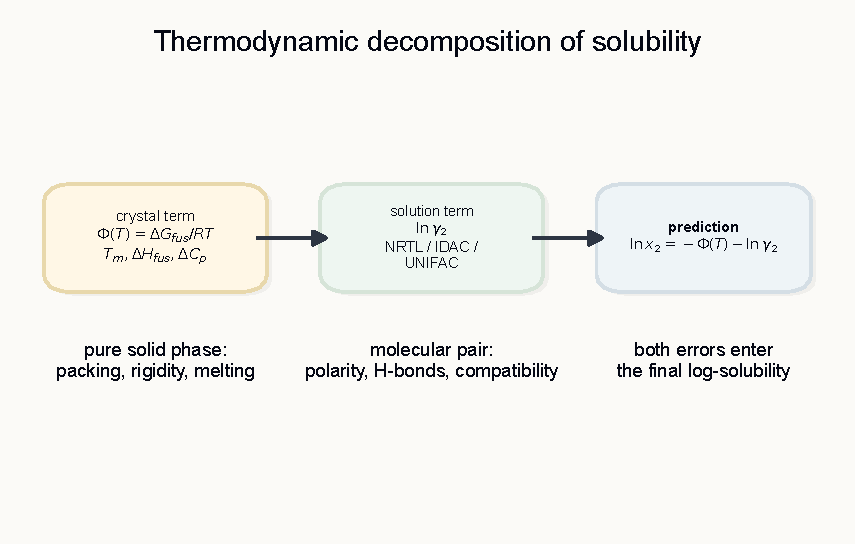
\includegraphics[width=0.92\textwidth]{sle_decomposition_schematic.pdf}
\caption{Разложение предсказания растворимости на кристаллический вклад $\Phi(T)$ и вклад активности $-\ln\gamma_2$. Именно это разложение делает промежуточные параметры проверяемыми.}
\end{figure}

\section{Модели и обучение}

DirectGNN и TGNN-Solv используют одну и ту же идею молекулярного представления: из графов вещества и растворителя строятся векторы молекул, затем формируется парное представление. Различается только выходной путь. DirectGNN сразу выдаёт $\ln x_2$. TGNN-Solv предсказывает кристаллические параметры, параметры активности, решает SLE и затем применяет ограниченную поправку к физическим параметрам.

Главное численное сравнение в отчёте относится к базовому MPNN-варианту, то есть к графовой сети с передачей сообщений. Более сложные блоки --- GraphGPS, TIMP, контрастивное выравнивание по параметрам Хансена, маршрутизация по типам растворителей и дескрипторное расширение --- реализованы как исследовательская инфраструктура~\cite{velickovic2018,vaswani2017,rampasek2022,schutt2018}. Их польза по средней ошибке пока не доказана; в диагностических запусках TIMP-варианты оставались хуже MPNN-базы. Основной результат нельзя объяснять этими блоками.

Для TIMP это особенно важно. Разделение сообщений на дисперсионный и полярный каналы является физически мотивированным индуктивным смещением, но оно может уменьшать выразительность модели. Поэтому отрицательный результат TIMP следует проверять не только по MAE, но и линейной пробой: если физико-химические дескрипторы хорошо читаются на обучающей части и плохо на тестовой, проблема в переносимости каналов; если плохо уже на обучении, каналам не хватает выразительности.

Обучение TGNN-Solv устроено поэтапно. Сначала вспомогательные физические свойства помогают инициализировать кристаллическую и активностную ветви. Затем включается полный SLE-путь и основная ошибка по растворимости. На последнем этапе выполняется тонкая настройка с меньшим шагом. Функция ошибки содержит основную ошибку по $\ln x_2$ и вспомогательные члены для кристаллических свойств, IDAC, температурной формы и регуляризации. Отсутствующие физические метки маскируются.

У такой схемы есть внутренний риск. Кристаллическая ветвь получает прямые метки $\Tm$ и частично $\dHfus$, а ветвь активности чаще получает только косвенный остаток через SLE и переносимый IDAC-сигнал. Из-за этого модель может сначала хорошо настроить представление одиночной молекулы под кристалл, а затем оставить парное взаимодействие недообученным. Градиентное голодание перекрёстного внимания является симптомом этого дисбаланса, а не только технической ошибкой реализации.

В ответ на этот риск в код добавлен опциональный диагностический штраф на согласованную компенсацию ошибок ветвей на строках, где одновременно известны $\Tm$, $\dHfus$ и $\ln x_2$:
\begin{equation*}
    \mathcal L_{\mathrm{decorr}}
    =
    \mathrm{corr}(\delta\Phi,\delta\gamma)^2,
    \qquad
    \delta\Phi=\Phi_{\mathrm{pred}}-\Phi_{\mathrm{true}},
    \qquad
    \delta\gamma=
    \ln\gamma_{2,\mathrm{pred}}
    -
    \left(
        -\ln x_{2,\mathrm{true}}-\Phi_{\mathrm{true}}
    \right).
\end{equation*}
Смысл этого члена --- штрафовать не просто большую ошибку каждой ветви по отдельности, а именно их согласованную антикорреляцию. Он не входит в поддерживаемый baseline по умолчанию и на основном scaffold-корпусе слишком разрежён для обычного mixed-batch обучения, поэтому пока проверялся только как малая абляция на crystal-known probe, где все строки имеют совместные кристаллические метки.

Технические детали реализации --- явные водороды для воды, отдельный IDAC-поток, UNIFAC-псевдометки, температурные компоненты функции ошибки, градиентные проверки и вспомогательные ветви --- вынесены в приложения. В основном тексте важен их статус: они реализованы, но не все доказали вклад в итоговую MAE. Оси и внутренние подписи на графиках оставлены на английском языке, потому что рисунки напрямую воспроизводят расчётные графики; русские подписи под рисунками переводят их смысл.

\section{Основные результаты}

Все численные сравнения ниже относятся к одному поддерживаемому запуску или одному диагностическому протоколу. Доверительные интервалы не оценены; близкие различия по MAE нельзя считать статистически доказанными. Три знака после запятой сохранены для воспроизводимости результатов, а не как заявление о такой точности.

\begin{center}
\small
\begin{tabularx}{\textwidth}{P{0.30\textwidth}rrY}
\toprule
Модель & $\mae$ & $\Rtwo$ & Интерпретация \\
\midrule
DirectGNN & 1.652 & 0.478 & лучшая средняя ошибка в текущем контролируемом сравнении \\
Случайный лес, гибридные признаки & 1.722 & 0.449 & сильный ненейросетевой ориентир \\
TGNN-Solv & 1.741 & 0.438 & физический путь уступает DirectGNN на $0.089$ MAE \\
\bottomrule
\end{tabularx}
\end{center}

Интерпретируемость физической модели не отменяет этот результат. В текущем виде TGNN-Solv проигрывает DirectGNN по средней ошибке на новых каркасах. Научный статус работы: физический путь реализован, диагностируем и имеет понятные точки отказа, но пока не превосходит прямую модель.

\textbf{Отдельный локальный режим с известным кристаллом даёт другой результат.} На внутреннем \emph{crystal-known probe} физическая модель впервые обходит прямую без тестового оракула:
\begin{center}
\small
\begin{tabular}{lrrrr}
\toprule
Режим & $\mae$ & $\Rtwo$ & bias & $\sigma(\hat y)/\sigma(y)$ \\
\midrule
TGNN-Solv, standard & 0.601 & 0.633 & $+0.087$ & 0.518 \\
DirectGNN & 0.818 & 0.569 & $-0.370$ & 0.463 \\
TGNN-Solv, oracle-train & 0.567 & 0.512 & $+0.393$ & 0.472 \\
TGNN-Solv, forced oracle eval & 1.244 & $-0.113$ & $+0.118$ & 0.074 \\
TGNN-Solv, oracle-train + forced oracle eval & 1.251 & $-0.234$ & $+0.450$ & 0.076 \\
\bottomrule
\end{tabular}
\end{center}

Этот микропротокол не заменяет главный scaffold-результат, потому что содержит только $35/7/8$ строк в train/val/test. Но именно он показывает, в каком режиме физический путь уже даёт содержательный выигрыш: когда кристаллические параметры наблюдаемы и задача не сводится целиком к восстановлению скрытого кристалла из структуры.

Более лёгкие разбиения показывают, что основная трудность связана с новым веществом и новым каркасом:
\begin{center}
\small
\begin{tabular}{lrrl}
\toprule
Разбиение & $\mae$ & $\Rtwo$ & Вывод \\
\midrule
Случайные строки & 0.166 & 0.987 & почти повторение виденных пар \\
Случайные пары & 0.783 & 0.806 & компоненты обычно уже видны \\
Новый растворитель & 0.732 & 0.735 & относительно легче \\
Новое вещество & 1.642 & 0.420 & основная сложность \\
Новый каркас & 1.703 & 0.462 & новая структура и смещение распределения \\
\bottomrule
\end{tabular}
\end{center}

Число $0.166$ для случайных строк не следует читать как реальное качество на новых системах. В таком разбиении соседние температуры и часто те же пары вещество--растворитель попадают и в обучение, и в тест. Это проверка интерполяции внутри уже виденной химии, а не прогноза новой молекулы.

Температурная проверка даёт другой важный результат. В режиме известной пары аппроксимация Вант-Гоффа резко превосходит нейросетевые диагностические модели:
\begin{center}
\small
\begin{tabular}{lrrl}
\toprule
Метод & $\mae$ (один протокол) & $\Rtwo$ & Правильное направление \\
\midrule
Вант-Гофф, режим известной пары & 0.368 & 0.887 & 99.0\% \\
Линейная зависимость от $T$ & 0.414 & 0.850 & 99.0\% \\
Случайный лес с температурой & 1.290 & 0.658 & 40.4\% \\
DirectGNN, малый бюджет & 1.619 & 0.283 & не считалась \\
TGNN-Solv, малый бюджет & 1.945 & 0.060 & не считалась \\
\bottomrule
\end{tabular}
\end{center}

Для нейросетевых диагностических моделей в этой проверке сохранялись MAE и $\Rtwo$, но не доля правильного направления. Аудит протокола показал $100\%$ пересечение пар между низкотемпературной обучающей и высокотемпературной тестовой частями. Вант-Гофф здесь является физическим ориентиром в режиме известной пары: он показывает наличие температурной формы в данных, но не перенос этой формы на новые молекулы.

\begin{figure}[!htbp]
\centering
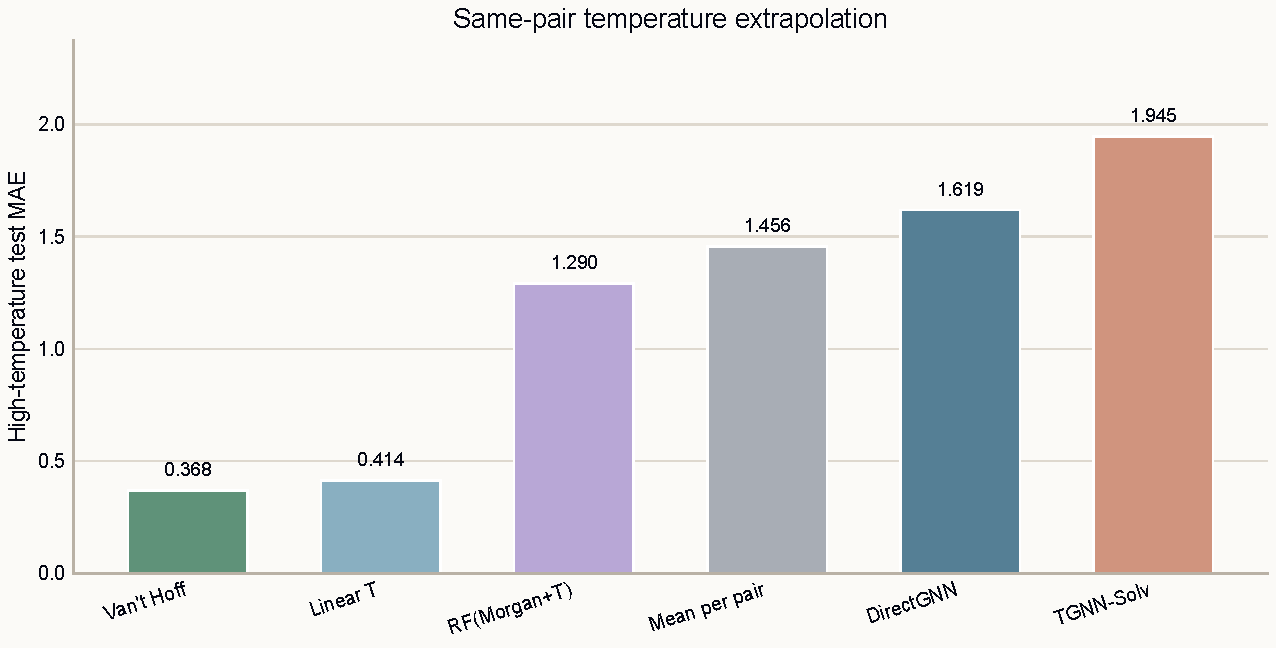
\includegraphics[width=0.88\textwidth]{temperature_extrapolation_baseline_comparison.pdf}
\caption{Температурная экстраполяция внутри известной пары. Аналитическая форма Вант-Гоффа служит физическим ориентиром, но не заменяет прогноз новых пар.}
\end{figure}

\section{Почему физический путь проигрывает в текущем запуске}

Начать стоит с самого общего эффекта: все модели сжимают диапазон предсказаний. На каркасном тесте стандартное отклонение истинных значений равно $3.119$, а стандартные отклонения предсказаний трёх основных моделей составляют только $67$--$70\%$ этого масштаба. Левый хвост $\ln x_2<-15$ остаётся особенно трудным: MAE там равна $7.78$ у DirectGNN, $8.14$ у случайного леса и $8.22$ у TGNN-Solv на $60$ строках.

\begin{center}
\small
\begin{tabularx}{\textwidth}{P{0.25\textwidth}rrrr}
\toprule
Модель & $\sigma(y)$ & $\sigma(\hat y)$ & $\sigma(\hat y)/\sigma(y)$ & $r_{\mathrm{slope}}$ \\
\midrule
DirectGNN & 3.119 & 2.183 & 0.700 & 0.129 \\
Случайный лес, гибридные признаки & 3.119 & 2.096 & 0.672 & 0.223 \\
TGNN-Solv & 3.119 & 2.157 & 0.692 & $-0.015$ \\
\bottomrule
\end{tabularx}
\end{center}

Корреляция наклонов в последнем столбце посчитана для $763$ пар с как минимум тремя температурными точками. У TGNN-Solv она практически нулевая: модель не восстанавливает температурную структуру и слишком сильно тянется к среднему.

Более показательный эффект --- NRTL-ветвь не различает пары. В температурном диагностическом запуске стандартное отклонение предсказаний TGNN-Solv равно $0.582$ при истинном $2.560$. Параметр $\tau_{12}$ меняется между парами меньше чем на $10^{-4}$ ($\sigma\approx4.8\cdot10^{-5}$), а финальная поправка к физическому выходу почти нулевая. Модель выдаёт почти одинаковый вклад активности для разных систем и фактически приближается к кристаллическому расчёту с малой постоянной поправкой. Это ровно тот режим, где физический путь теряет смысл: активность должна различать совместимые и несовместимые пары вещество--растворитель.

Здесь есть два уровня проблемы. Первый --- концентрационный: большинство SLE-строк лежит в области малой растворимости, где данные видят главным образом одну величину, $\ln\gamma_2^\infty(T)$, а не отдельные $\tau_{12}$, $\tau_{21}$ и $\alpha$. Второй --- информационный: кристаллический блок имеет прямые метки, а активность чаще получает только остаток после вычитания кристалла. Это делает активностную ветвь слабее обеспеченной данными и объясняет, почему она склонна схлопываться к почти постоянной поправке.

Поправочный блок тоже требует отдельной диагностики. Он ограниченно меняет физические параметры и заново решает SLE, что сохраняет форму расчёта. Но если исходная NRTL-ветвь почти постоянна, большая поправка к $\tau$ может фактически компенсировать ошибку кристаллического уровня через активность. Это численно полезно, но физически неоднозначно. Поэтому для новых прогонов добавлен журнал величин поправки. В малой проверке с прямым пределом активности поправочный блок не делал основную работу: средняя величина финальной поправки к $\ln x_2$ была около $0.001$, а разброс поправки к параметру активности составлял лишь около $0.13\%$ от разброса самого параметра.

\begin{figure}[!htbp]
\centering
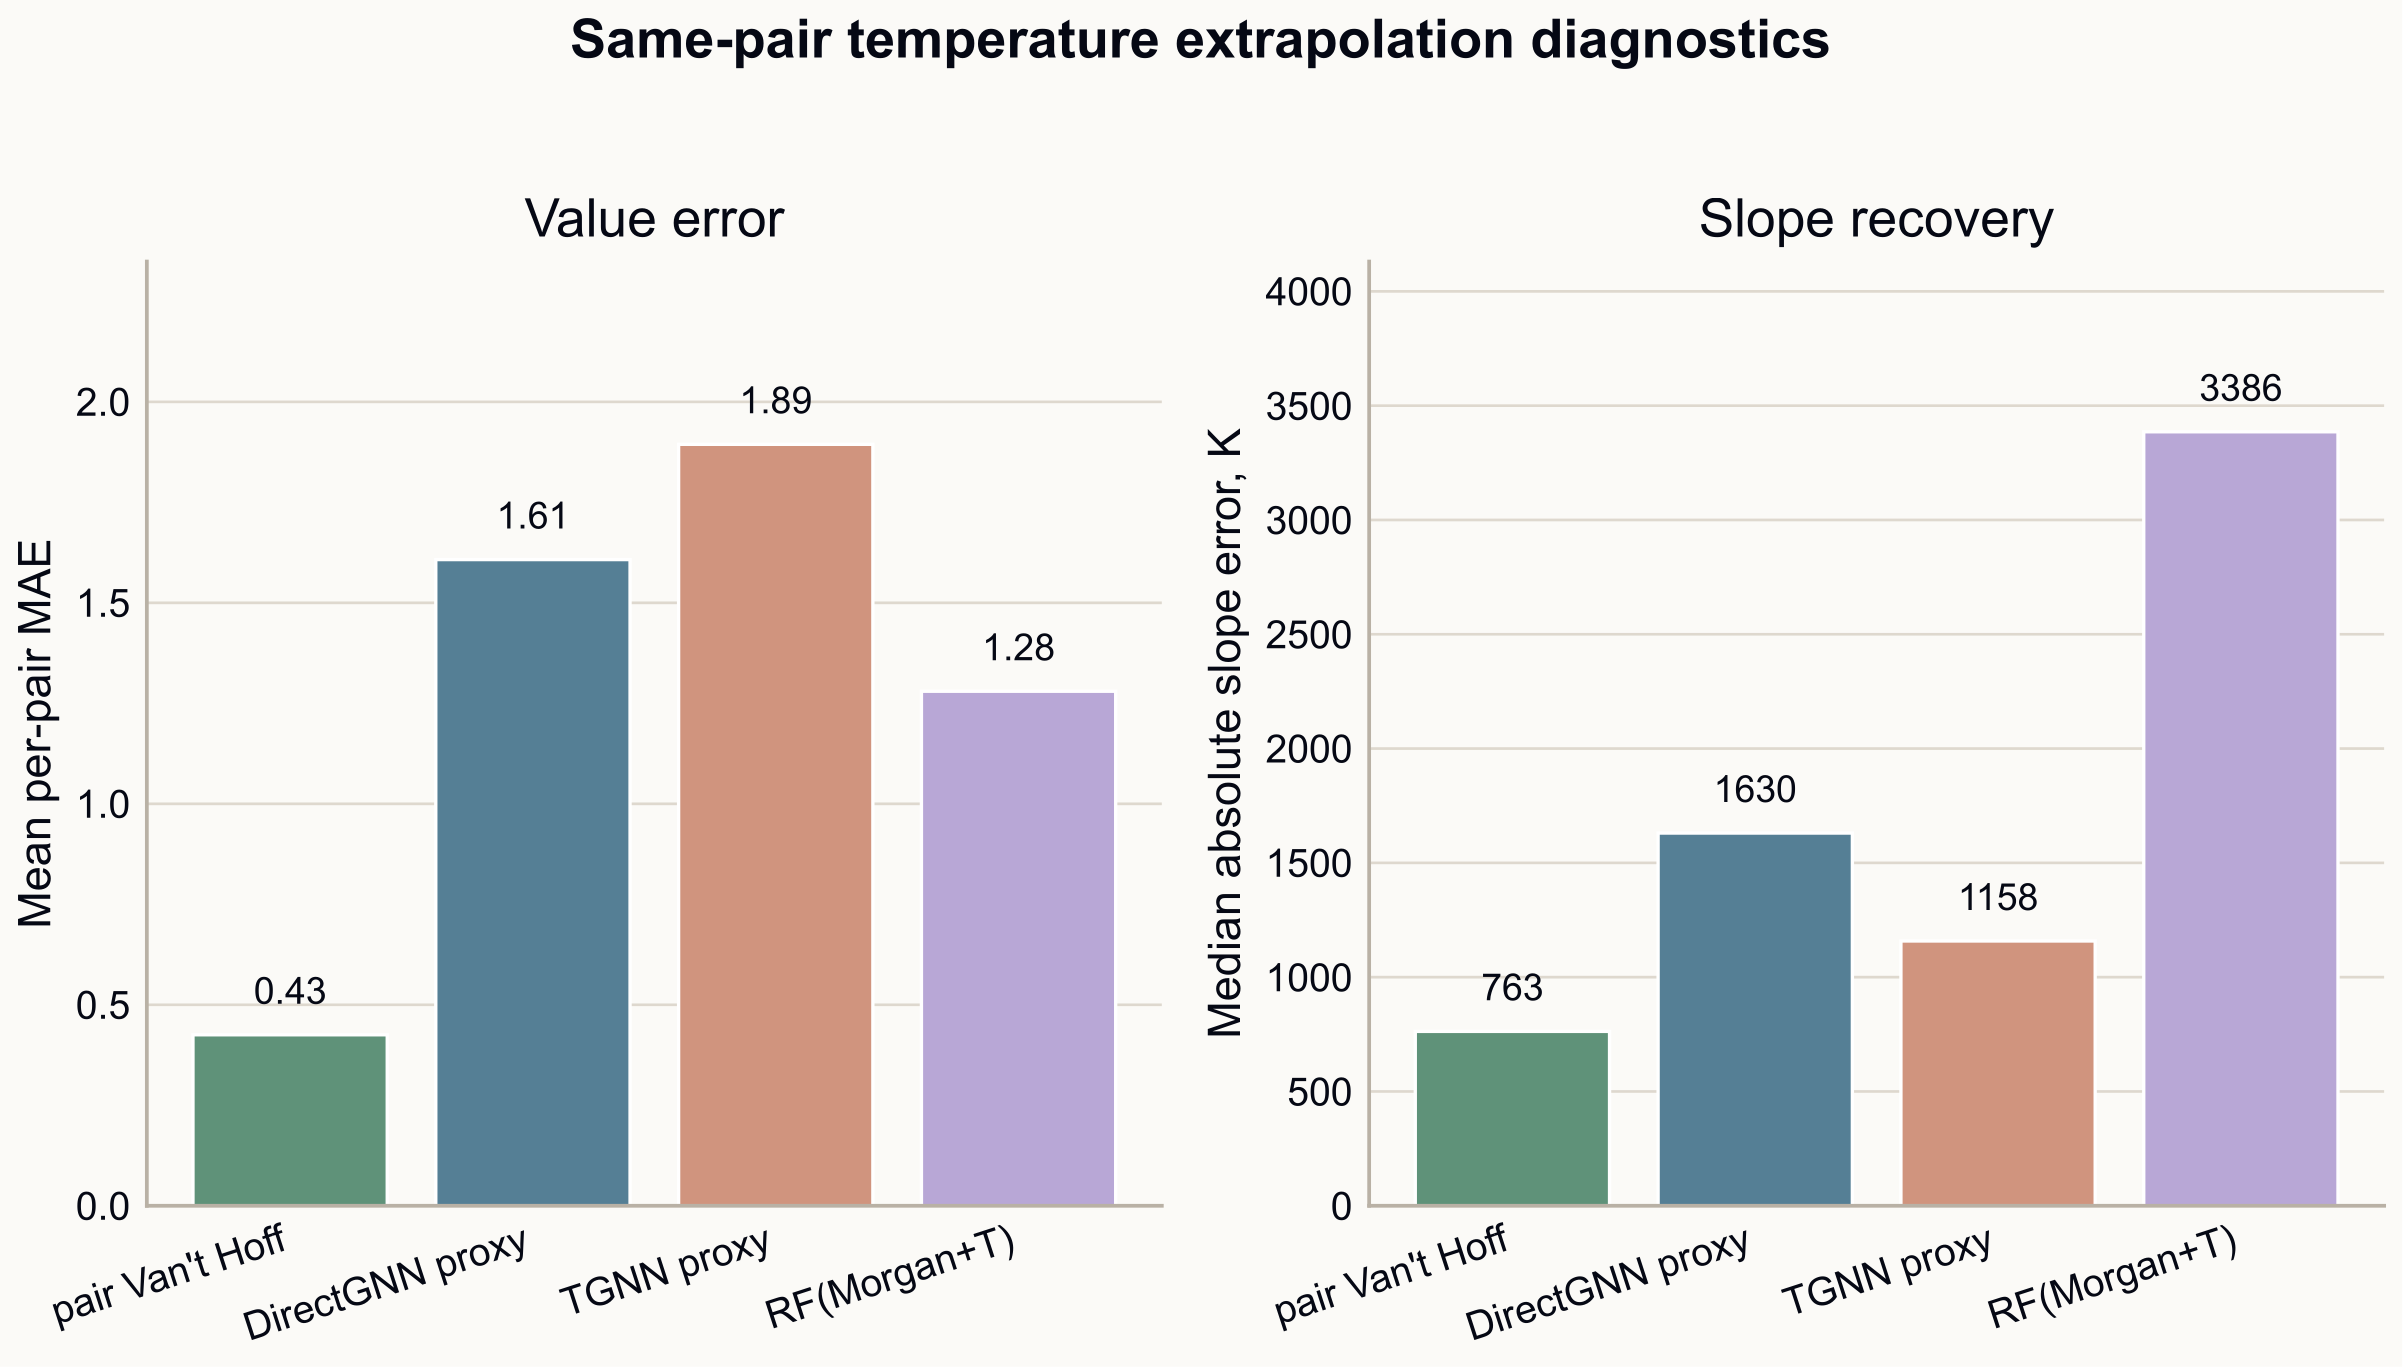
\includegraphics[width=0.92\textwidth]{temperature_slope_recovery_diagnostics_raster.png}
\caption{Диагностика уровня и наклона на температурной экстраполяции. TGNN-Solv частично восстанавливает знак наклона, но проигрывает по уровню $\ln x_2$ и даёт сжатые предсказания.}
\end{figure}

Новая малая проверка с прямым пределом активности уточнила картину. Физический путь восстанавливает температурный наклон лучше прямой модели: средняя ошибка наклона составляет около $1471\,\mathrm K$ против $1947\,\mathrm K$ у DirectGNN, то есть улучшение порядка $24\%$. Но уровень кривой хуже: среднее смещение по $\ln x_2$ равно $-1.396$, тогда как у DirectGNN оно близко к нулю ($+0.011$). Такой сдвиг означает систематическое занижение растворимости примерно в $\exp(1.4)\approx4$ раза. Поэтому итоговая MAE хуже не потому, что физическая форма полностью неверна, а потому что кривая поставлена на неправильный абсолютный уровень.

\begin{center}
\small
\begin{tabularx}{\textwidth}{P{0.31\textwidth}rrrr}
\toprule
Малая модель & MAE & $R^2$ & Среднее смещение & MAE наклона, K \\
\midrule
DirectGNN & 3.053 & 0.207 & $+0.011$ & 1947 \\
TGNN-Solv, полная NRTL & 3.416 & 0.111 & $-1.628$ & 1471 \\
TGNN-Solv, прямой $\ln\gamma^\infty$ & 3.236 & 0.194 & $-1.396$ & 1471 \\
TGNN-Solv, $\ln\gamma^\infty$ + смещение + парная потеря & 3.225 & 0.225 & $-1.431$ & 1506 \\
TGNN-Solv, то же + хвостовая потеря & 2.862 & 0.318 & $-0.430$ & 1491 \\
\bottomrule
\end{tabularx}
\end{center}

Проверка обучаемого глобального смещения активности и увеличенного веса вспомогательной парной потери дала смешанный результат. Она немного улучшила тестовую MAE ($3.236\to3.225$) и $R^2$ ($0.194\to0.225$), но не уменьшила среднее смещение уровня: оно осталось около $-1.4$. Температурный наклон при этом остался лучше, чем у DirectGNN, но немного ухудшился относительно исходной прямой параметризации активности ($1471\to1506\,\mathrm K$). Значит, один только прямой парный сигнал повышает ранжирование, но не решает главную ошибку уровня.

Постфактум-калибровка уровня подтвердила этот диагноз. Если сдвинуть тестовые предсказания варианта со смещением и парной потерей на медианное смещение, оценённое по валидационной части, MAE уменьшается с $3.225$ до $2.856$, а $R^2$ растёт с $0.225$ до $0.315$. Оракульный сдвиг, подобранный уже по тесту, даёт MAE $2.768$ и служит только верхней оценкой пользы калибровки. Биновая калибровка по предсказанному значению была проверена отдельно и не стала улучшением: пять валидационных бинов дали MAE $3.027$, а линейная, устойчивая и изотоническая калибровки также не превзошли глобальный медианный сдвиг по MAE. Поэтому честный вывод узкий: заметная часть ошибки находится в уровне кривой, но простая биновая постобработка не решает сжатие диапазона.

Более полезной оказалась не постобработка, а изменение функции потерь. В малом прогоне с фиксированными повышенными весами для хвостов распределения TGNN-Solv снизила MAE с $3.225$ до $2.862$, подняла $R^2$ с $0.225$ до $0.318$ и уменьшила среднее смещение с $-1.431$ до $-0.430$. На том же малом срезе это лучше взвешенной DirectGNN ($\mae=3.053$, $\Rtwo=0.207$), а преимущество по температурному наклону сохраняется: $1491\,\mathrm K$ против $1947\,\mathrm K$. Но это не означает, что сжатие диапазона устранено. Отношение $\sigma(\hat y)/\sigma(y)$ у хвостовой версии равно только $0.592$ против $0.703$ у предыдущей физической версии; модель стала точнее по уровню и ранжированию, но диапазон всё ещё сжат. По бинам истинной растворимости знак ошибки также меняется: крайний левый хвост завышается, а более растворимые строки занижаются. Значит, следующий шаг --- локализовать, завышены ли $\Phi(T)$, $\ln\gamma^\infty$, или оба вклада, а не добавлять ещё один глобальный сдвиг.

Прямое разложение смещения на кристаллическую и активностную части в этой малой проверке пока невозможно: в соответствующей тестовой части нет строк, где одновременно есть надёжные $\Tm$ и $\dHfus$. Косвенный сигнал всё же есть. Среднее предсказанное $\ln\gamma^\infty$ на тесте выше, чем на валидационной части, а большой $\Phi(T)$ остаётся основным вкладом уровня. Поэтому следующий шаг --- не ещё один глобальный сдвиг, а раздельная проверка кристаллической ветви и ветви активности на строках с внешними или надёжными кристаллическими параметрами.

Такая раздельная проверка была дополнительно выполнена на внутреннем \emph{crystal-known probe}: из обучающей части выделены только строки, где одновременно известны $\Tm$ и $\dHfus$; после стратифицированного разбиения получен микросрез $35/7/8$ строк для train/val/test. Этот тест слишком мал для самостоятельного численного вывода и содержит всего два кристаллических режима на тесте, но он полезен как локальный диагноз. На нём обычный TGNN-Solv даёт $\mae=0.601$, $\Rtwo=0.633$ и среднее смещение $+0.087$, тогда как сопоставимый DirectGNN даёт $\mae=0.818$, $\Rtwo=0.569$ и смещение $-0.370$. При этом диапазон остаётся сжатым у обеих моделей: $\sigma(\hat y)/\sigma(y)=0.518$ у TGNN-Solv и $0.463$ у DirectGNN. Следовательно, локальный выигрыш физического пути идёт через ранжирование и bias, а не через полное восстановление амплитуды.

Главный структурный результат этой проверки --- не только победа TGNN-Solv, но и механизм, которым она достигается. Принудительная oracle-подстановка истинных $\Tm$ и $\dHfus$ в уже обученный TGNN-Solv ухудшает результат до $\mae=1.244$ и почти схлопывает диапазон предсказаний: отношение $\sigma(\hat y)/\sigma(y)$ падает до $0.074$. Отдельное обучение той же конфигурации с oracle-подстановкой в train-time улучшает test-MAE лишь умеренно, до $0.567$, но при этом даёт заметное положительное смещение $+0.393$ и более низкий $\Rtwo=0.512$. Комбинация train-time oracle и forced-oracle eval даёт худший итог: $\mae=1.251$ и отрицательный $\Rtwo=-0.234$. Значит, модель выучивает согласованное решение, в котором кристаллическая и активностная ветви компенсируют ошибки друг друга.

Эта компенсация теперь измерена явно. Для стандартного TGNN-Solv на всех $8$ тестовых строках crystal-known probe знаки $\delta\Phi=\Phi_{\mathrm{pred}}-\Phi_{\mathrm{true}}$ и $\delta\gamma=\ln\gamma_{2,\mathrm{pred}}-\ln\gamma_{2,\mathrm{req}}$ противоположны; корреляция между ними равна $-0.876$. Среднее $\abs{\delta\Phi+\delta\gamma}$ составляет $0.590$, а расхождение между итоговой ошибкой физической суммы и финальной ошибкой после ограниченной коррекции равно лишь около $0.024$. Иначе говоря, bounded correction здесь не меняет вывод: основная согласованность достигается уже на уровне суммы $-\Phi-\ln\gamma_2$. После forced-oracle eval кристаллическая ошибка почти зануляется ($\delta\Phi\approx1.7\cdot10^{-4}$), но среднее $\abs{\delta\Phi+\delta\gamma}$ вырастает до $1.242$. Это и есть количественное подтверждение \emph{coupled decomposition}: отдельно правильный кристалл не спасает, если активностная ветвь была обучена компенсировать другой кристаллический режим.

В ответ на этот диагноз был проверен и прямой штраф
\(
\mathcal L_{\mathrm{decorr}}=\mathrm{corr}(\delta\Phi,\delta\gamma)^2
\)
на том же микросрезе. Таблица ниже важна именно как отрицательный результат: численно он даёт лишь слабое улучшение standard-качества, но почти не меняет саму структуру компенсации.

\begin{center}
\small
\begin{tabularx}{\textwidth}{P{0.32\textwidth}rrrr}
\toprule
Вариант TGNN-Solv на crystal-known probe & MAE & $\sigma(\hat y)/\sigma(y)$ & $\mathrm{corr}(\delta\Phi,\delta\gamma)$ & MAE forced-oracle \\
\midrule
Без $L_{\mathrm{decorr}}$ & 0.601 & 0.518 & $-0.876$ & 1.244 \\
$L_{\mathrm{decorr}}$, вес 0.05 & 0.601 & 0.518 & $-0.876$ & 1.243 \\
$L_{\mathrm{decorr}}$, вес 0.20 & 0.599 & 0.521 & $-0.876$ & 1.243 \\
$L_{\mathrm{decorr}}$, вес 0.50 & 0.597 & 0.525 & $-0.876$ & 1.242 \\
\bottomrule
\end{tabularx}
\end{center}

Эта абляция позволяет сказать больше, чем просто ``эффект мал''. При росте веса штрафа среднее $\abs{\delta\Phi+\delta\gamma}$ уменьшается лишь с $0.590$ до $0.585$, а forced-oracle gap даже немного растёт: разница MAE между forced-oracle и standard увеличивается примерно с $0.642$ до $0.646$. Следовательно, прямой batch-level штраф на антикорреляцию ошибок ветвей сам по себе не размыкает coupled decomposition. Это ожидаемо: проблема не в том, что оптимизатор выбирает ``не тот'' антикоррелированный угол, а в том, что текущие SLE-данные сами по себе недоопределяют разложение на $\Phi(T)$ и $\ln\gamma_2$. Регуляризация не создаёт новую информацию. Реально разрывать такую связь могут только независимые данные на ветви: конечноконцентрационные activity-измерения, надёжные внешние кристаллические параметры для большой доли тестовых молекул или широкие многотемпературные ряды. На этом микросрезе штраф работает как мягкая регуляризация уровня, но не решает плохую идентифицируемость разложения.

Проверка IDAC как размыкателя этой связи в точной постановке пока невозможна. Для crystal-known probe точное пересечение с текущим расширенным IDAC-корпусом равно нулю не только по парам, но даже по отдельным растворяемым веществам и растворителям. Поэтому правильный следующий шаг теперь уже не общий призыв ``добавить больше IDAC'', а отдельный протокол, где SLE- и IDAC-наблюдения пересекаются по одной и той же паре или по явно контролируемой близкой химии.

Частично первый из этих маршрутов уже материализован в виде открытого ThermoML activity-контура, а теперь и в виде targeted pair-coverage artifact с measurement-level harvest. Этот audit показывает ещё более точную границу, чем раньше. Общее exact pair overlap между SLE и ThermoML существует и даже не мало по меркам корпуса, но почти всё это покрытие занято composition-like, density, viscosity и другими сопутствующими свойствами. Если смотреть только на candidate supervision для activity-ветви, картина снова становится жёсткой: property-level overlap даёт лишь $16$ directed pairs, а usable measurement-backed overlap --- только $15$, причём direct activity остаётся solvent-side, solution-thermo сигнал покрывает лишь единичные пары, VLE-like overlap почти отсутствует, а \(H^E\) не даёт ни одной exact SLE pair. Поэтому bottleneck теперь нужно формулировать уже не как общее ``нужно больше GE/VLE'' и не как полное pair-level несовпадение корпусов, а как дефицит нужных property families на уже частично пересекающихся парах. Сам по себе новый artifact ещё не снимает идентифицируемость, но он переводит следующий шаг в конкретную воспроизводимую задачу: идти по списку measurement-backed candidate-missing SLE pairs и целенаправленно искать или собирать для них именно те внешние термодинамические наблюдения, которые действительно информируют ветвь активности.

Кристаллический вклад даёт отдельный источник ошибки. На строках без кристаллических меток ошибка выше, чем на строках с известным $\Tm$: у TGNN-Solv $1.81$ против $1.51$, у DirectGNN $1.71$ против $1.45$. В диагностическом TGNN-прогоне на строках с известным $\Tm$ ошибка предсказания $\Tm$ около $47.5\,\mathrm K$, а для $\dHfus$ контрольной метки в каркасном тесте нет. Оценка чувствительности в приложении~\ref{app:sensitivity} показывает масштаб проблемы: ошибка $30\,\mathrm K$ в $\Tm$ даёт вклад около $0.53$ в $\ln x_2$, а ошибка $5\,\mathrm{kJ/mol}$ в $\dHfus$ --- около $0.68$. Эти величины сравнимы с разницей между моделями и объясняют, почему физический путь может проигрывать прямой регрессии даже при правильном уравнении SLE. Контрольная подстановка внешних кристаллических параметров для $128$ совпавших строк снизила среднюю ошибку температурного TGNN-расчёта с $2.786$ до $1.155$. Часть больших ошибок действительно находится в кристаллическом уровне, хотя одна эта подстановка не закрывает всю задачу.

Поправка $\Delta C_p^{\mathrm{fus}}$ остаётся самым неопределённым кристаллическим параметром. Оценка показывает, что для высокоплавких молекул её вклад может достигать порядка единицы в $\ln x_2$, но прямых меток $\Delta C_p^{\mathrm{fus}}$ в текущем обучении практически нет. Значит, такая ветвь может одновременно убирать систематическую ошибку и добавлять шум. Её нужно проверять как отдельную абляцию: нулевая поправка, фиксированная физическая оценка и обучаемая поправка должны сравниваться на одном протоколе.

Наконец, есть проблема потока градиента к парному взаимодействию. Короткая проверка показала, что NRTL-голова получает ненулевой градиент, но блок парного взаимодействия TGNN-Solv получает заметно более слабый сигнал, чем соответствующий блок DirectGNN. Эта проблема не исчезла сама после перехода к прямому пределу активности и отсоединения кристаллической ветви: в малом тесте отношение нормы градиента парного блока TGNN-Solv к DirectGNN составило около $0.069$. Вспомогательная парная потеря подняла это отношение до $0.268$ при весе $0.2$, до $0.667$ при весе $0.5$ и до $1.33$ при весе $1.0$. Отдельное отсечение кристаллических параметров от SLE-градиента почти не изменило результат при весе $0.2$. Значит, главный рычаг --- сила прямого парного сигнала; следующий вопрос состоит в том, какой вес улучшает MAE, не превращая физическую модель в скрытую прямую регрессию.

Итог этой диагностики не сводится к «плохой оптимизации». Проблема глубже: физический путь пытается одновременно решать две задачи с разным объёмом информации. Температурная экстраполяция внутри известной пары хорошо ограничена данными. Перенос на новое вещество требует предсказать кристалл и активность из структуры, причём активность получает меньше прямых меток. Поэтому следующий строгий результат должен сначала показать выигрыш физического пути в одном чётко заданном режиме, а не смешивать режим известной пары и перенос на новую химию в одной средней MAE.

\section{Статус рабочих гипотез}

Ниже собран сводный статус тех гипотез, которые уже проверены текущими поддерживаемыми и диагностическими артефактами. Таблица не заменяет подробные разделы выше, а фиксирует их итог в компактной форме.

Здесь важно различать уже подтверждённые выводы и рабочие гипотезы, которые пока поддержаны только малым прогоном или одной диагностикой. В таблице сознательно сохранены промежуточные статусы вроде «частично поддержана» и «предварительно поддержана»: на этом этапе важнее честно отделить устойчивый факт от правдоподобного механизма, чем искусственно довести все формулировки до окончательного вердикта.

{\small
\setlength{\LTleft}{0pt}
\setlength{\LTright}{0pt}
\begin{longtable}{P{0.29\textwidth}P{0.20\textwidth}P{0.43\textwidth}}
\caption{Сводный статус основных гипотез после текущей серии проверок.}\label{tab:hypotheses-status}\\
\toprule
Гипотеза & Статус & Основание \\
\midrule
\endfirsthead
\toprule
Гипотеза & Статус & Основание \\
\midrule
\endhead
\bottomrule
\endfoot
\bottomrule
\endlastfoot
Кристаллический вклад является существенным источником ошибки & Частично поддержана & Ошибка выше без кристаллических меток; внешняя подстановка для $128$ строк снижает ошибку TGNN-расчёта с $2.786$ до $1.155$, а train-time oracle на crystal-known probe улучшает MAE лишь с $0.601$ до $0.567$: вклад есть, но он не исчерпывает проблему без активности. \\
Компенсация между $\Phi(T)$ и $\ln\gamma_2$ количественно подтверждена & Поддержана & На standard crystal-known probe знаки $\delta\Phi$ и $\delta\gamma$ противоположны на всех $8$ строках, корреляция равна $-0.876$, а forced-oracle eval почти зануляет $\delta\Phi$, но повышает среднее $\abs{\delta\Phi+\delta\gamma}$ с $0.590$ до $1.242$. \\
Прямой decorrelation-loss сам по себе размыкает coupled decomposition & Не подтверждена & На crystal-known probe sweep весов $0.05/0.20/0.50$ улучшил MAE лишь с $0.601$ до $0.597$, но $\mathrm{corr}(\delta\Phi,\delta\gamma)$ осталась около $-0.876$, а forced-oracle MAE --- около $1.242$. \\
NRTL-ветвь в текущем запуске плохо различает пары & Поддержана & Малый разброс $\tau_{12}$ и почти нулевая корреляция температурных наклонов показывают слабый парный сигнал. \\
Три параметра NRTL идентифицируются из SLE-данных & Не подтверждена & В малорастворимом пределе SLE видит в основном $\ln\gamma_2^\infty(T)$; отдельные $\tau_{12}$, $\tau_{21}$ и $\alpha$ плохо разделяются. \\
Прямая параметризация $\ln\gamma_2^\infty(T)$ сама по себе достаточна для победы над прямой моделью & Не подтверждена & В малом прогоне она улучшила TGNN-Solv относительно полной NRTL-ветви и наклонов DirectGNN, но проиграла по абсолютному уровню. \\
Хвостовая функция потерь помогает физическому пути & Предварительно поддержана & В малом прогоне она снизила MAE TGNN-Solv до $2.862$ и обошла DirectGNN на том же срезе, но не устранила сжатие диапазона и требует повторения на полном бюджете. \\
Температурная форма в данных действительно есть & Поддержана в режиме известной пары & Вант-Гофф даёт $\mae=0.368$ при $100\%$ пересечении пар; перенос на новые пары остаётся открытым. \\
Вспомогательная парная ветка улучшает итоговую точность & Частично поддержана & Короткая проверка показывает управляемый рост парного градиента с весом потери; лучший малый MAE получен вместе с хвостовой потерей, но полноразмерной абляции ещё нет. \\
Поправочный блок улучшает физическую интерпретируемость & Открыта & Нужно проверить, не компенсирует ли он ошибки кристалла через параметры активности. \\
eNRTL является необходимым следующим шагом & Не подтверждена & Для ключевых солевых примеров сначала нужно отделить ошибку кристаллического вклада от описания контактной ионной пары. \\
\end{longtable}
}

\section{Химические примеры}

Средняя ошибка не объясняет, почему модель ошибается. Химические примеры разделяют разные режимы: неверный кристаллический уровень, недоученная активность, контактная ионная пара, полярно-аполярное несоответствие и недооценённая специфическая сольватация. Контактная ионная пара означает, что катион и анион остаются рядом как связанная сольватированная единица, а не расходятся как полностью диссоциированные ионы. Подробные структуры и полный разбор приведены в приложении~\ref{app:detailed-cases}; здесь оставлена карта интерпретаций.

Дельфинидин-хлорид особенно важен как пример преждевременного вывода. Его температурные ряды согласованы, источник описывает чистые растворители, а не подкисленные смеси, но в обработанных строках нет $\Tm$ и $\dHfus$. Такая система сначала требует аудита кристаллического вклада, и только после этого --- обсуждения активности или eNRTL. Для низкодиэлектрических органических растворителей дельфинидин-хлорид, вероятно, существует преимущественно как контактная ионная пара; это осложняет графовое представление, но не превращает систему автоматически в полностью диссоциированный электролит. Есть и ещё один риск: флавилиевые соли могут иметь pH- и средозависимые равновесия форм. Если растворённая фаза фактически является смесью форм, то одно бинарное SLE-уравнение описывает её только как эффективную систему.

{\small
\setlength{\LTleft}{0pt}
\setlength{\LTright}{0pt}
\begin{longtable}{P{0.27\textwidth}P{0.33\textwidth}P{0.34\textwidth}}
\caption{Что показывают химические примеры.}\label{tab:chemical-examples}\\
\toprule
Система & Наблюдаемая ошибка & Интерпретация \\
\midrule
\endfirsthead
\toprule
Система & Наблюдаемая ошибка & Интерпретация \\
\midrule
\endhead
\bottomrule
\endfoot
\bottomrule
\endlastfoot
N-tert-butylacrylamide--formamide & TGNN-Solv существенно лучше DirectGNN & Нейтральная амидная пара с малым требуемым активностным сдвигом; физическое ограничение уровня помогает. \newline\emph{Что это говорит о модели:} SLE-путь может быть полезен, когда активностная поправка мала и главным остаётся уровень кривой. \\
Дельфинидин-хлорид--ацетон/этанол & Все модели сильно завышают растворимость & Соль с контактной ионной парой и отсутствующими $\Tm,\dHfus$; по этой ошибке нельзя отдельно вывести необходимость eNRTL. \newline\emph{Что это говорит о модели:} для солей без кристаллических параметров сначала нужен аудит $\Phi(T)$, а не усложнение активности. \\
Ксилит--толуол & TGNN-Solv сохраняет форму, но завышает уровень & Полиол в аполярном растворителе требует большого неблагоприятного вклада активности; почти постоянная NRTL-ветвь его не создаёт. \newline\emph{Что это говорит о модели:} текущая активностная ветвь не различает резко несовместимые пары. \\
Витамин K3 / менадион--бензол & TGNN-Solv занижает растворимость & Возможна недооценка благоприятной ароматической совместимости, но без подстановки истинных кристаллических параметров это неотделимо от ошибки $\Phi(T)$. \newline\emph{Что это говорит о модели:} недостающий благоприятный вклад активности и ошибка кристалла могут давать одинаковый знак ошибки. \\
Борнеол--п-ксилол & TGNN-Solv занижает растворимость & Ошибка может идти как от недостающего благоприятного вклада активности, так и от завышенного кристаллического штрафа. \newline\emph{Что это говорит о модели:} гидрофобно-ароматическая совместимость требует отдельной проверки активности и кристаллической подстановки. \\
\end{longtable}
}

\section{Что уже проверено до полноразмерного обучения}

Часть работы можно было выполнить без дорогого полного обучения: анализ уже сохранённых предсказаний, проверка сжатия диапазона, метрики по бинам растворимости, парные температурные наклоны, аудит кристаллических меток, покрытие UNIFAC и малые обучающие проверки новых функций ошибки. Эти проверки не заменяют основной эксперимент, но они заранее уточнили, что нужно измерять в следующем запуске.

Практический итог этих проверок следующий. Взвешенная MAE уменьшает глобальное смещение DirectGNN на малом диагностическом срезе, но не устраняет сжатие диапазона. Прямая параметризация $\Phi(T)=a+b/T$ для строк без надёжных кристаллических параметров улучшает крайний левый хвост, но не улучшает среднюю ошибку в коротком прогоне. Прямое предсказание $\ln\gamma_2^\infty(T)$ улучшает малую TGNN-модель относительно полной NRTL-ветви и даёт более правильный температурный наклон, однако вносит сильное отрицательное смещение уровня. Обучаемое глобальное смещение активности вместе с более сильной парной потерей почти не меняет MAE ($3.236\to3.225$) и не убирает среднее смещение. Простая калибровка уровня по валидационной части заметно снижает ошибку, но биновая калибровка по предсказанному значению не превзошла глобальный медианный сдвиг. Фиксированная хвостовая функция потерь дала лучший малый результат без постобработки: $\mae=2.862$, $\Rtwo=0.318$ против $3.053$ и $0.207$ у DirectGNN на том же срезе. При этом диапазон предсказаний остался сжатым, так что результат нужно читать как предварительный выигрыш за счёт уровня и ранжирования, а не как закрытую проблему экстраполяции. Crystal-known probe добавил новый локальный факт: стандартный TGNN-Solv уже лучше DirectGNN по MAE ($0.601$ против $0.818$), но forced-oracle eval ломает это преимущество и количественно подтверждает компенсацию между $\Phi$ и $\ln\gamma_2$. Прямой decorrelation-loss на том же probe улучшил MAE лишь до $0.597$ и почти не изменил ни корреляцию $\delta\Phi$ и $\delta\gamma$, ни forced-oracle провал, так что пока это лишь слабая регуляризация, а не решение coupled decomposition. Более реалистичная rescue-проверка внешнего COSMO-side потока показала, что внешний pair/activity-сигнал уже существует, но не делает forced-oracle картину чище. Exact-joint supervision на том же heldout-rescue протоколе оказалась более сильным структурным рычагом: режим $w100$ держит main test почти на уровне baseline ($3.253\to3.249$), но ухудшает crystal-standard ($2.038\to2.161$); после исправления масштаба aux-loss лучший чистый компромисс даёт $w025$ ($3.221/2.223/1.340$ для main/crystal/oracle), а $w025+\mathrm{COSMO}\,w005$ даёт лучшие oracle-диагностики ($1.322$ и $\abs{\delta\Phi+\delta\gamma}=1.311$), но ещё худший standard transfer ($3.311/2.275$). Значит, проблема теперь локализована точнее: exact-joint действительно ослабляет coupled decomposition, но делает это через target, построенный по экспериментальному кристаллу, тогда как standard solver использует предсказанный кристалл. Поэтому текущий приоритетный следующий шаг уже не в дальнейшем ослаблении sidecar, а в двухэтапном обучении кристаллической и активностной ветвей или в режиме координатного спуска. Отдельная малая проверка режима $\ln\gamma^\infty=\ln\gamma^\infty_{\mathrm{UNIFAC}}+\Delta_{\mathrm{NN}}$ показала низкое покрытие на переносе ($25.2\%/4.4\%/6.1\%$ для train/val/test) и не дала обнадёживающего старта по валидации, поэтому UNIFAC сейчас остаётся слабым приором, а не главным следующим рычагом. Внешняя подстановка кристаллических параметров резко улучшает часть температурных примеров, но ухудшает ксилит и салициловую кислоту; значит, активность раствора и фазовая форма остаются самостоятельными источниками ошибки. Попытка проверить IDAC как размыкатель компенсации на текущем crystal-known probe упирается в нулевое пересечение с IDAC-корпусом, так что для этого вывода понадобится новый специально собранный протокол.

Покрытие UNIFAC оказалось слишком малым, чтобы считать его универсальным приором: около $8.6\%$ строк каркасного теста. Поэтому его влияние нужно ограничивать строками с распознанными группами или учитывать маской доверия. Иначе приор может добавлять шум именно там, где новая химия и так плохо покрыта.

\section{Итог}

Работа не доказывает общего превосходства TGNN-Solv. Её текущий результат точнее и интереснее: на главном scaffold-протоколе физический путь всё ещё уступает DirectGNN, но на внутреннем crystal-known probe впервые даёт локальный выигрыш без тестового оракула. Одновременно эта же проверка показывает, почему локальный выигрыш нельзя переинтерпретировать как чистую физическую интерпретируемость: модель использует согласованную компенсацию между кристаллическим вкладом и активностью раствора. Более реалистичный heldout-rescue пакет с внешним COSMO-side потоком и exact-joint supervision делает эту двойственность жёстче: activity-sidecar действительно ослабляет oracle-компенсацию, но как только цель для $\ln\gamma_2$ строится через экспериментальный кристалл, crystal-standard качество ухудшается. Значит, следующий барьер уже не в отсутствии sidecar-сигнала, а в несогласованности activity-target и ошибающейся кристаллической ветви.

\begin{table}[!htbp]
\centering
\caption{Минимальный следующий пакет проверок.}
\small
\begin{tabularx}{\textwidth}{P{0.30\textwidth}Y}
\toprule
Проверка & Зачем нужна \\
\midrule
Несколько случайных инициализаций & Проверить устойчивость разрыва TGNN-Solv и DirectGNN. \\
Полная температурная экстраполяция & Понять, переносит ли TGNN-Solv форму Вант-Гоффа на новые пары, а не только интерполирует известные пары. \\
Контрольная подстановка кристалла & Отделить ошибку $\Phi(T)$ от ошибки активности раствора. \\
Логирование NRTL и парных градиентов & Проверить, перестала ли NRTL-ветвь быть почти постоянной и получает ли парное взаимодействие достаточный сигнал. \\
Аудит поправочного блока & Понять, какие физические параметры он меняет и не маскирует ли ошибку кристалла через активность. \\
Двухэтапное обучение crystal/activity & Проверить, исчезнет ли ухудшение crystal-standard, если сначала обучить и заморозить кристаллическую ветвь на строках с известными $\Tm,\dHfus$, затем обучать ветвь активности с exact-joint supervision и только потом делать короткую поочерёдную донастройку ветвей. \\
IDAC-протокол с пересечением по парам и UNIFAC-абляции & Проверить, действительно ли IDAC размыкает компенсацию между $\Phi$ и $\ln\gamma_2$, а не остаётся только физически правдоподобной регуляризацией без парного пересечения. \\
Сравнение NRTL с прямой $\ln\gamma_2^\infty(T)$ & Проверить, нужна ли трёхпараметрическая NRTL-форма в малорастворимом режиме. \\
\(\Delta C_p^{\mathrm{fus}}\)-абляция & Отделить полезную теплоёмкостную поправку от шума необученного параметра. \\
\bottomrule
\end{tabularx}
\end{table}

Следующий вопрос теперь узкий и проверяемый: исчезнет ли ухудшение crystal-standard, если разнести обучение по ветвям и перестать учить activity-часть против движущейся ошибки кристалла. Ближайший технический шаг поэтому уже не в выборе ещё одного локального веса sidecar, а в двухэтапном расписании: сначала отдельное обучение кристаллической ветви на строках с известными $\Tm,\dHfus$, затем её заморозка и exact-joint обучение ветви активности против фиксированного предсказанного $\Phi$, после чего --- одна-две короткие итерации координатного спуска. Для этого всё ещё нужен вычислительный ресурс, которого сейчас нет. Именно поэтому этот отчёт является запросом на следующий этап, а не финальным утверждением о превосходстве модели. Если следующий этап не подтвердит выигрыш, физический путь в текущей NRTL-постановке следует рассматривать прежде всего как диагностический инструмент, а не как лучший предсказатель средней растворимости. Но теперь это уже более сильный диагностический инструмент: он не только локализует точки отказа, но и показывает конкретный режим, где физическое ограничение начинает работать.

\clearpage

\appendix
\makeatletter
\renewcommand\thesection{\AlphAlph{\value{section}}}
\renewcommand\thesubsection{\thesection.\arabic{subsection}}
\renewcommand\theHsection{app.\AlphAlph{\value{section}}}
\renewcommand\theHsubsection{\theHsection.\arabic{subsection}}
\makeatother

\section*{Приложения}
\addcontentsline{toc}{section}{Приложения}

Приложения разделены на три группы. A--C содержат глоссарий, вычислительные результаты, аудиты и графики. D--M содержат математическое обоснование SLE-пути, чувствительности и идентифицируемости. N--AI фиксируют планируемые доработки, инженерные проверки и пределы применимости. Разделы второй и третьей групп не следует читать как дополнительные экспериментальные победы модели: они объясняют, что уже проверено теоретически и что нужно проверять в следующем вычислительном этапе.

\section*{Вычислительные результаты}
\addcontentsline{toc}{section}{Вычислительные результаты}

\section{Обозначения и термины}\label{app:terms}

\begin{center}
\begin{tabularx}{\textwidth}{P{0.24\textwidth}Y}
\toprule
Термин & Краткое пояснение \\
\midrule
$\ln x_2$ & Логарифм мольной доли растворяемого вещества; основная целевая величина. \\
Твёрдо-жидкое равновесие & Равенство химических потенциалов вещества в кристалле и насыщенном растворе; физическая основа TGNN-Solv. \\
Графовая модель & Модель, которая читает молекулу как граф атомов и химических связей. \\
Молекулярный каркас & Остов молекулы по Мёрко; разбиение по каркасам проверяет перенос на новые структурные классы. \\
NRTL & Модель коэффициентов активности в неидеальном бинарном растворе; в малорастворимых SLE-системах главным наблюдаемым пределом часто является $\ln\gamma_2^\infty$. \\
IDAC & Коэффициент активности при бесконечном разбавлении; частичный прямой сигнал для ветви активности, но не полное определение всех NRTL-параметров. \\
Контрольная подстановка & Диагностический расчёт, где часть физических параметров берётся из измерений; иногда называется оракульным расчётом. \\
Поддерживаемый запуск & Полный цикл обучения и оценки с зафиксированной конфигурацией, зерном, весами, предсказаниями и метриками. \\
Диагностический прогон & Короткая проверка отдельного механизма; такой прогон не заменяет основное сравнение моделей по качеству. \\
\bottomrule
\end{tabularx}
\end{center}

\section{Подробные химические примеры температурных систем}\label{app:detailed-cases}

Названия систем в этом разделе сохранены в формате, используемом в данных и на рисунках. Для распространённых веществ русское название добавляется в тексте; подписи структур оставлены в том же стиле, что и сами рисунки.

\paragraph{N-tert-butylacrylamide--formamide.}
Это нейтральный акриламид с одной амидной донорно-акцепторной группой и объёмным трет-бутильным фрагментом. Formamide, или формамид, --- малый сильнополярный протонный растворитель. Специфическая сольватация амидного центра здесь ожидаема, но требуемая поправка активности в выбранных высокотемпературных точках мала: средний требуемый вклад по диагностике около $0.29$ в $\ln x_2$. TGNN-Solv выигрывает у DirectGNN ($\mae=0.29$ против $2.52$), потому что физический путь удерживает уровень кривой около наблюдаемого значения. DirectGNN в запуске с малым бюджетом переоценивает благоприятность полярной пары и предсказывает слишком высокую растворимость. Что это говорит о модели: SLE-ограничение может помогать в системах, где активностный вклад невелик и главное --- не потерять уровень температурной кривой.

\begin{figure}[H]
\centering
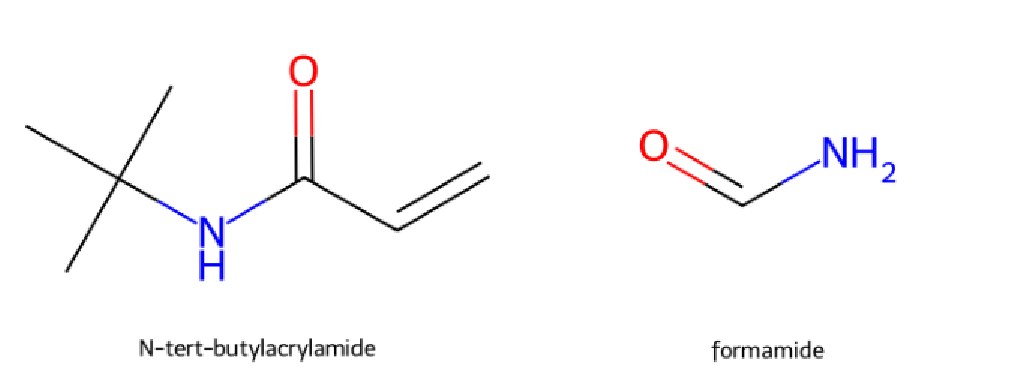
\includegraphics[width=0.58\textwidth]{example_system_n_tert_butylacrylamide_formamide.pdf}
\caption{Структуры пары N-tert-butylacrylamide--formamide. Это пример, где физическое ограничение уровня помогает TGNN-Solv.}
\label{fig:case-n-tert-butylacrylamide-formamide}
\end{figure}

\paragraph{2,4-dinitro-L-phenylalanine--water.}
Эта система устроена иначе. Вещество аминокислотоподобное: есть аминная и карбоксильная функциональность, две сильные нитро-группы и ароматическое ядро. Вода хорошо сольватирует полярные центры, но динитроароматический фрагмент и возможные протонированные/цвиттер-ионные формы делают уровень растворимости нетривиальным. TGNN-Solv здесь сильно завышает растворимость ($\mae=3.02$), тогда как DirectGNN предсказывает точнее ($\mae=0.36$). Интерпретация простая: физический путь в диагностическом запуске почти не использует NRTL-ветвь и не создаёт нужный положительный вклад активности, который должен сдвинуть кривую вниз. Что это говорит о модели: водные полярные системы нельзя описывать одним кристаллическим уровнем; ветвь активности должна создавать различимый штраф несовместимости.

\begin{figure}[H]
\centering
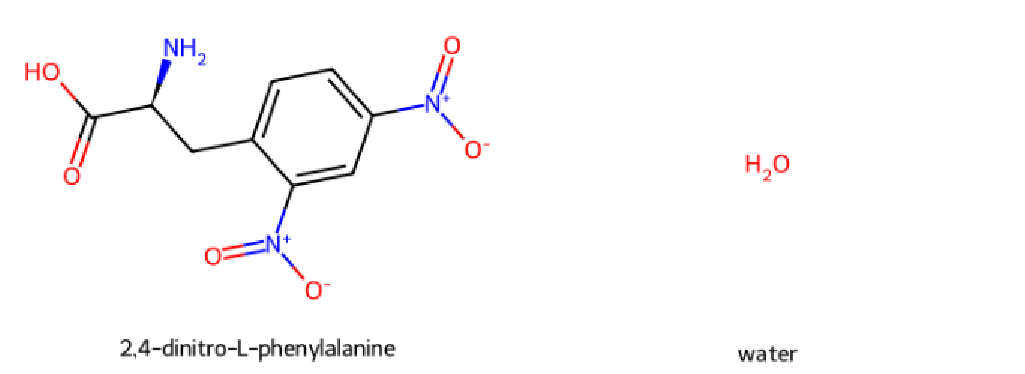
\includegraphics[width=0.58\textwidth]{example_system_2_4_dinitro_l_phenylalanine_water.pdf}
\caption{Структуры пары 2,4-dinitro-L-phenylalanine--water. Ошибка TGNN-Solv связана не с неправильным знаком температурного тренда, а с недостающим уровнем активности.}
\label{fig:case-dinitro-phenylalanine-water}
\end{figure}

\paragraph{Дельфинидин-хлорид--ацетон и дельфинидин-хлорид--этанол.}
Дельфинидин-хлорид --- флавилиевая соль: плоский катионный ароматический хромофор с несколькими фенольными группами и отдельный хлорид-анион. В ацетоне и этаноле это скорее режим контактной ионной пары, чем полностью диссоциированного электролита. Температурные ряды в исходных строках согласованы, так что эти данные нельзя объяснить только шумом измерений. В обработанных строках нет экспериментальных $\Tm$ и $\dHfus$; при таких масках TGNN-Solv передаёт в SLE-решатель кристаллические параметры, предсказанные из графа. Для флавилиевой соли, которая может разлагаться до обычного плавления, эта задача плохо определена. В ацетоне истинные значения лежат около $\ln x_2\approx -23$, а TGNN-Solv ошибается на $18.46$; в этаноле истинные значения около $-16$, ошибка TGNN-Solv равна $11.56$. Наблюдаемая ошибка смешивает неизвестный кристаллический уровень, представление контактной ионной пары и активность раствора, поэтому по одной этой системе нельзя делать вывод о необходимости eNRTL. Что это говорит о модели: солевые системы без надёжных кристаллических параметров должны получать отдельный флаг и отдельный срез метрик.

\begin{figure}[H]
\centering
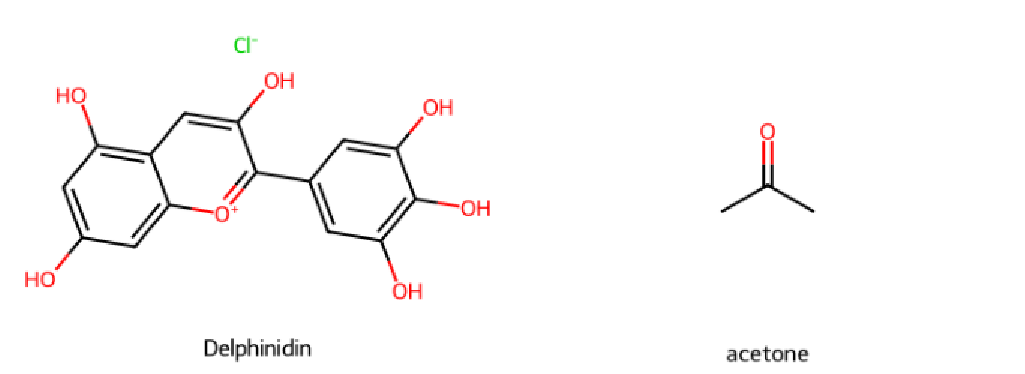
\includegraphics[width=0.58\textwidth]{example_system_delphinidin_acetone.pdf}
\caption{Структуры пары дельфинидин-хлорид--ацетон. Ацетон не даёт сильной протонной стабилизации хлорида; ошибка всех моделей является экстремальным завышением растворимости.}
\label{fig:case-delphinidin-acetone}
\end{figure}

\begin{figure}[H]
\centering
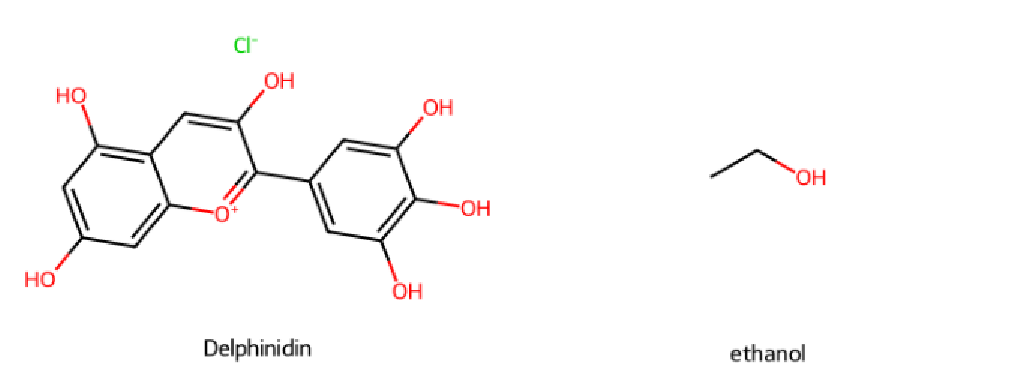
\includegraphics[width=0.58\textwidth]{example_system_delphinidin_ethanol.pdf}
\caption{Структуры пары дельфинидин-хлорид--этанол. Этанол может стабилизировать хлорид водородной связью, но отсутствие кристаллических параметров и солевая форма всё равно делают уровень растворимости трудным.}
\label{fig:case-delphinidin-ethanol}
\end{figure}

\paragraph{Xylitol--toluene.}
Xylitol, или ксилит, --- малый полиол с пятью гидроксильными группами. Toluene, или толуол, --- аполярный ароматический растворитель, который не может компенсировать плотную сетку водородных связей полиола. Истинная растворимость требует большого неблагоприятного вклада активности: полярно-аполярное несоответствие должно сдвигать $\ln x_2$ вниз. TGNN-Solv сохраняет похожий температурный наклон, но завышает уровень кривой примерно на $5.26$. Это типичный случай, где кристаллический член даёт форму, а почти константная NRTL-ветвь не добавляет нужное отталкивание раствора. Что это говорит о модели: текущий NRTL-блок не создаёт достаточный штраф для полярно-аполярной несовместимости.

\begin{figure}[H]
\centering
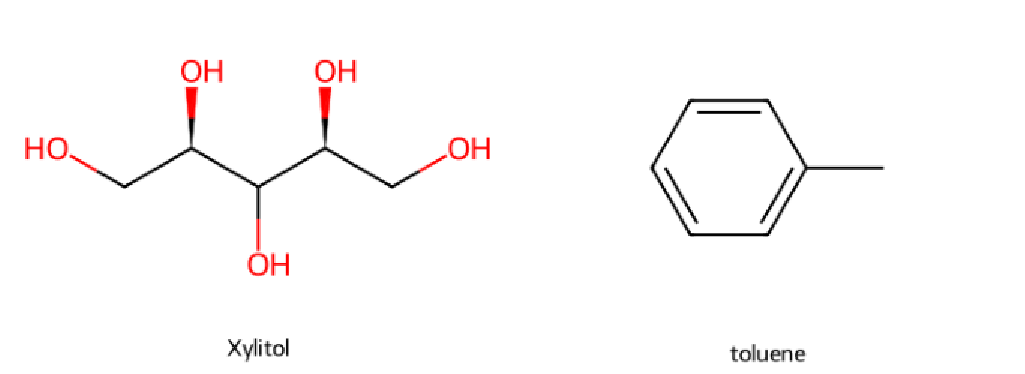
\includegraphics[width=0.58\textwidth]{example_system_xylitol_toluene.pdf}
\caption{Структуры пары xylitol--toluene. Главная химия ошибки --- сильное полярно-аполярное несоответствие.}
\label{fig:case-xylitol-toluene}
\end{figure}

\paragraph{Vitamin K3--benzene.}
Vitamin K3, или менадион, --- компактный гидрофобный нафтохинон: ароматическая поверхность, два карбонильных акцептора и ограниченная гибкость. Benzene, или бензол, совместим с ним по дисперсионным и $\pi$-взаимодействиям. Здесь ошибка TGNN-Solv имеет другой знак: модель недооценивает растворимость, то есть кривая оказывается слишком низкой. Вероятное объяснение --- физический путь слишком сильно опирается на кристаллический/идеальный вклад и не даёт достаточную благоприятную активностную поправку для ароматического растворителя. Альтернативное объяснение --- завышенный $\Phi(T)$; без контрольной подстановки истинных $\Tm$ и $\dHfus$ эти две причины нельзя строго разделить. Что это говорит о модели: при занижении растворимости нужно проверять не только активность, но и завышение кристаллического штрафа.

\begin{figure}[H]
\centering
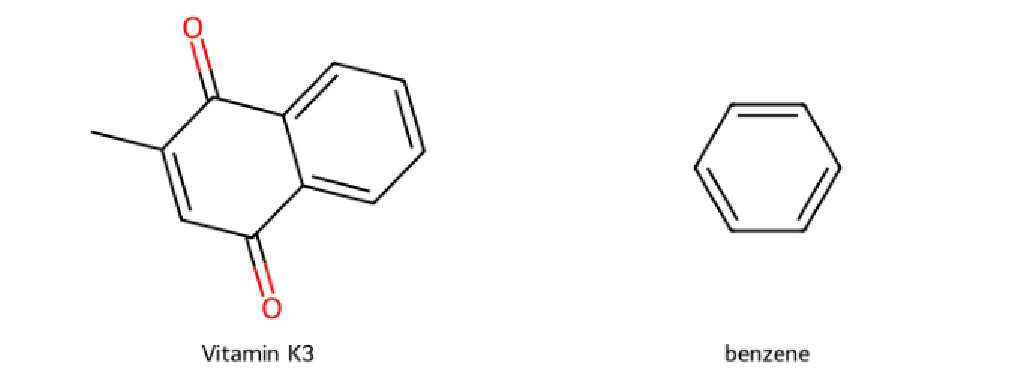
\includegraphics[width=0.58\textwidth]{example_system_vitamin_k3_benzene.pdf}
\caption{Структуры пары Vitamin K3--benzene. Случай относится не к левому хвосту плохой растворимости, а к недооценённой совместимости по дисперсионным и ароматическим взаимодействиям.}
\label{fig:case-vitamin-k3-benzene}
\end{figure}

\paragraph{Borneol--p-xylene.}
Borneol, или борнеол, --- компактный терпеновый спирт: большая гидрофобная поверхность и один гидроксильный центр. p-Xylene, или п-ксилол, --- аполярный ароматический растворитель; растворимость в значительной степени определяется дисперсионной совместимостью, а не сильной полярной сольватацией. TGNN-Solv снова предсказывает слишком низкий уровень ($\mae=3.31$ против $1.21$ у DirectGNN). Ошибка указывает на недостающий благоприятный вклад активности для гидрофобно-ароматических пар или на завышенный кристаллический штраф. Как и для Vitamin K3, разделить эти причины можно только контрольной подстановкой кристаллических параметров. Что это говорит о модели: гидрофобно-ароматические пары требуют контроля благоприятной активности, а не только хорошей температурной формы.

\begin{figure}[H]
\centering
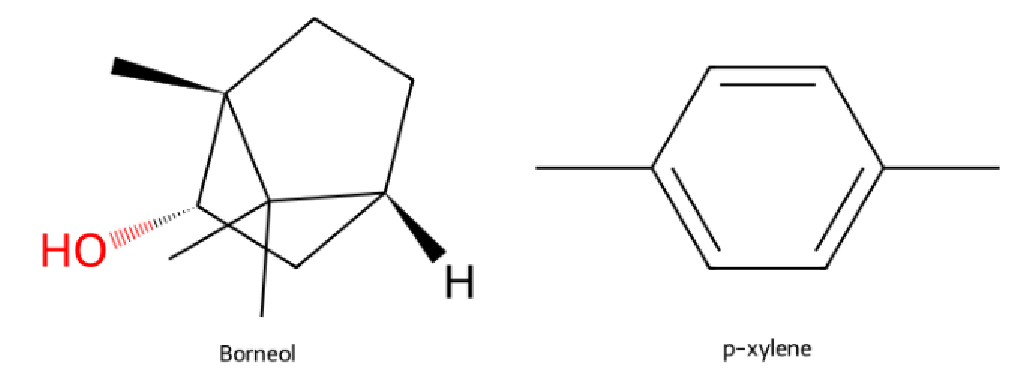
\includegraphics[width=0.58\textwidth]{example_system_borneol_p_xylene.pdf}
\caption{Структуры пары borneol--p-xylene. Ошибка TGNN-Solv связана с недооценкой благоприятной дисперсионной совместимости.}
\label{fig:case-borneol-p-xylene}
\end{figure}

\paragraph{o-Phthalic acid--DMAc.}
o-Phthalic acid, или о-фталевая кислота, содержит две карбоксильные группы в орто-положении и может образовывать сильные меж- и внутримолекулярные водородные связи. DMAc --- полярный апротонный растворитель с сильной карбонильной акцепторной группой. Наблюдаемая растворимость чувствительна к кислотно-основной и донорно-акцепторной ассоциации, а не только к общей полярности. TGNN-Solv недооценивает уровень растворимости: вероятно, кристаллический штраф или идеальная часть слишком велики, а благоприятная сольватация пары кислота--амид не выражена в NRTL-параметрах. Что это говорит о модели: специфическая ассоциация кислота--амид плохо сводится к почти постоянному коэффициенту активности.

\begin{figure}[H]
\centering
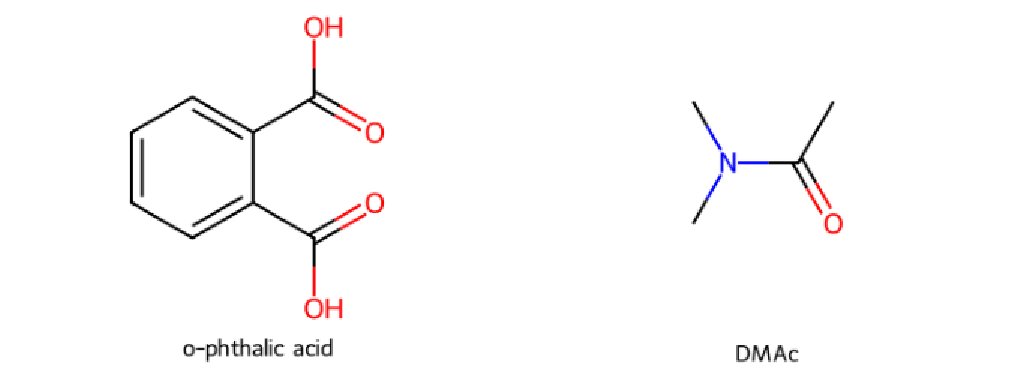
\includegraphics[width=0.58\textwidth]{example_system_o_phthalic_acid_dmac.pdf}
\caption{Структуры пары o-phthalic acid--DMAc. Система показывает чувствительность уровня растворимости к специфической ассоциации кислота--амид.}
\label{fig:case-o-phthalic-acid-dmac}
\end{figure}

\paragraph{m-Methylbenzoic acid--isobutanol.}
m-Methylbenzoic acid, или м-метилбензойная кислота, сочетает гидрофобное ароматическое кольцо и одну сильную карбоксильную группу. Isobutanol, или изобутанол, может и отдавать, и принимать водородные связи, а также имеет гидрофобный фрагмент. Это химически совместимая пара кислота--спирт. TGNN-Solv недооценивает растворимость примерно на $3.23$ в $\ln x_2$, что согласуется с той же причиной: ветвь активности не добавляет достаточно благоприятного вертикального сдвига для специфической ассоциации кислоты со спиртом. Что это говорит о модели: парная активность должна явно различать функционально совместимые кислотно-спиртовые пары.

\begin{figure}[H]
\centering
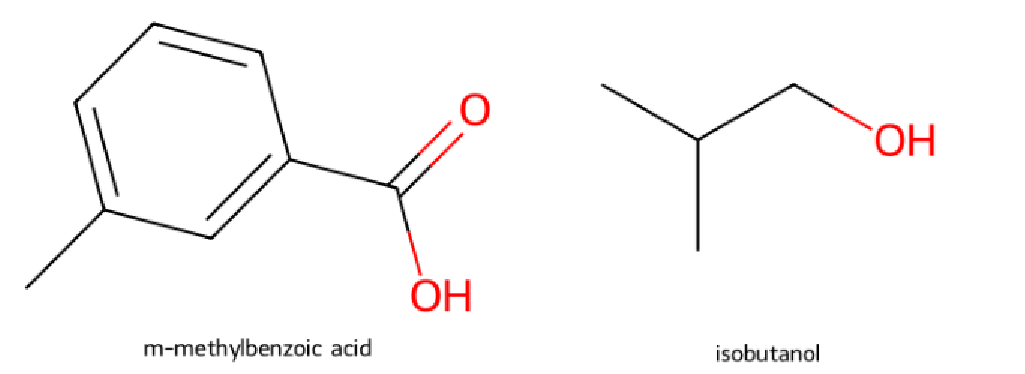
\includegraphics[width=0.58\textwidth]{example_system_m_methylbenzoic_acid_isobutanol.pdf}
\caption{Структуры пары m-methylbenzoic acid--isobutanol. Здесь важны взаимодействия кислота--спирт и гидрофобная совместимость.}
\label{fig:case-m-methylbenzoic-acid-isobutanol}
\end{figure}

\paragraph{Glutaric acid--acetic acid.}
Glutaric acid, или глутаровая кислота, --- гибкая алифатическая дикарбоновая кислота, а acetic acid, или уксусная кислота, одновременно растворитель и участник кислотных ассоциаций. В таких системах уровень растворимости может сильно меняться из-за димеризации, кислотно-кислотных контактов и конкуренции с кристаллической упаковкой. TGNN-Solv держит температурную форму лучше, чем абсолютный уровень: ошибка $3.12$ в основном является вертикальным сдвигом. Это ещё один пример того, что физический путь может знать направление температурной кривой, но не иметь достаточно выразительной активности раствора. Что это говорит о модели: правильный температурный наклон не гарантирует правильный уровень, если активность пары не идентифицирована.

\begin{figure}[H]
\centering
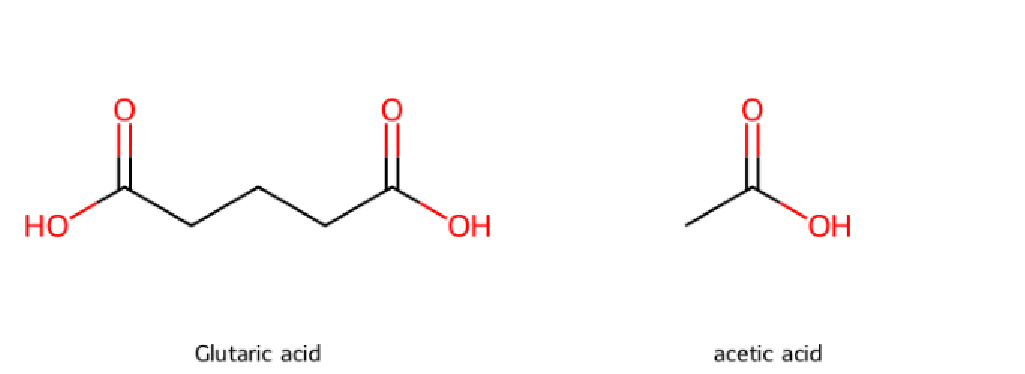
\includegraphics[width=0.58\textwidth]{example_system_glutaric_acid_acetic_acid.pdf}
\caption{Структуры пары glutaric acid--acetic acid. Ошибка уровня связана со специфической кислотной ассоциацией, а не с отсутствием температурного тренда.}
\label{fig:case-glutaric-acid-acetic-acid}
\end{figure}

\section{Экспериментальный и методический контекст}
\label{app:extended-experimental-context}

В этом приложении собраны проверочные сведения к численным выводам: состав корпуса, источники данных, режимы разбиения, внешние ориентиры, трудные химические классы, структурная диагностика, отрицательные результаты и степень подтверждения абляций.

\subsection{Корпус, источники и покрытие данных}

Основной корпус устроен сложнее, чем таблица «молекула--растворитель--число». В нём есть целевые строки растворимости, вспомогательные физические свойства, источники разного происхождения и повторные температурные ряды для одних и тех же пар. Из-за этого все метки хранятся с масками: строка может иметь растворимость, но не иметь $\Tm$; может иметь $\Tm$, но не иметь $\dHfus$; может быть IDAC-строкой и вообще не участвовать в ошибке по растворимости.

\begin{table}[!htbp]
\centering
\caption{Состав обработанного корпуса, используемого программами обучения и оценки.}
\label{tab:app-dataset-composition}
\small
\begin{tabular}{lr}
\toprule
Показатель & Значение \\
\midrule
Все строки в обработанных таблицах & $127\,088$ \\
Строки с целевой растворимостью & $108\,287$ \\
Уникальные растворяемые вещества с метками растворимости & $1\,525$ \\
Уникальные растворители с метками растворимости & $212$ \\
Уникальные пары вещество--растворитель с метками растворимости & $12\,129$ \\
Диапазон температур в строках растворимости & $243.15$--$425.77\,\mathrm K$ \\
Медианная температура & $303.15\,\mathrm K$ \\
Среднее число температурных строк на пару & $8.93$ \\
Медианное число температурных строк на пару & $9$ \\
Полные точные дубликаты троек вещество--растворитель--температура & $0$ \\
Конфликтующие дубликаты таких троек & $0$ \\
\bottomrule
\end{tabular}
\end{table}

Отсутствие конфликтующих полных дублей важно для интерпретации ошибок. Значения MAE порядка $1.6$ нельзя объяснить тем, что одинаковые тройки часто имеют разные экспериментальные значения. Главная трудность находится в другом: в переносе на новые вещества, новые молекулярные каркасы и новые температурные области.

\begin{figure}[!htbp]
\centering
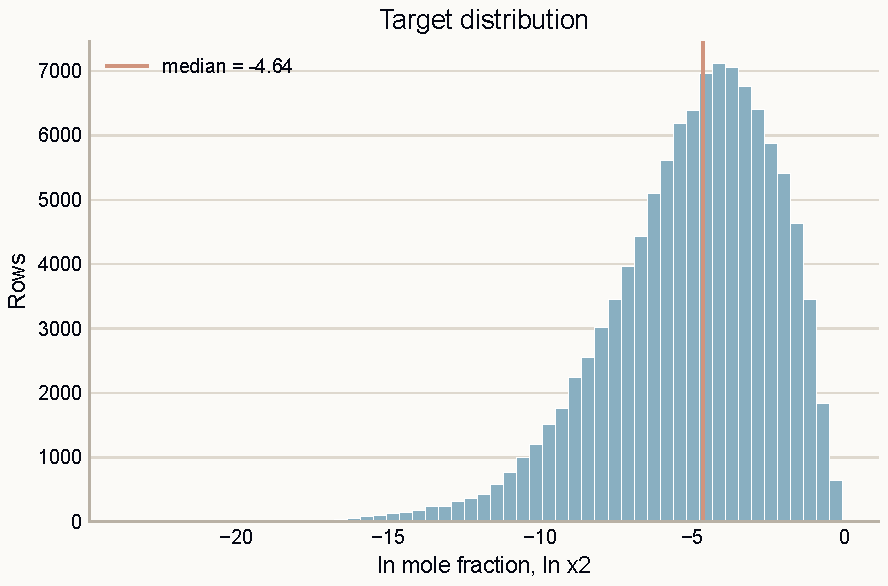
\includegraphics[width=0.70\textwidth]{corpus_lnx2_histogram.pdf}
\caption{Распределение целевой величины $\ln x_2$. Логарифмическая шкала необходима, потому что корпус содержит одновременно хорошо растворимые и практически нерастворимые системы.}
\label{fig:app-corpus-lnx2}
\end{figure}

\begin{figure}[!htbp]
\centering
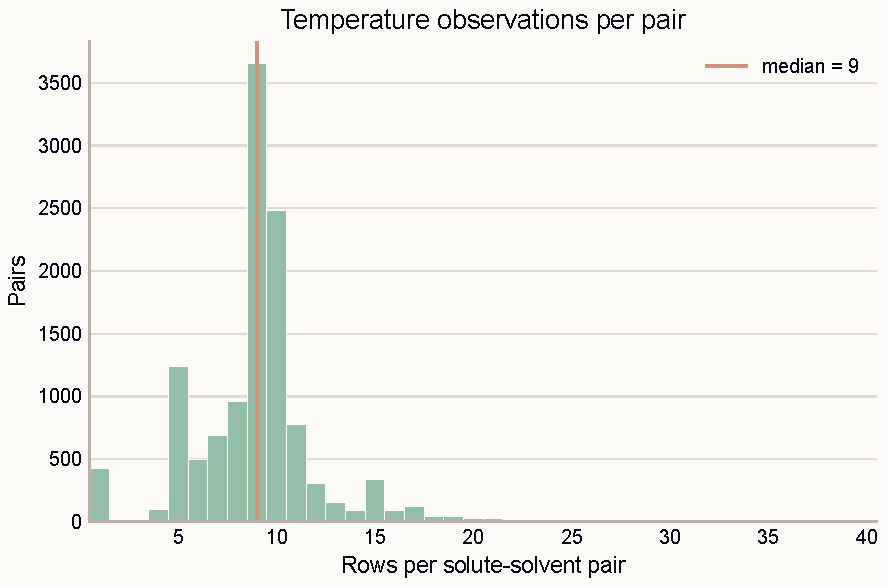
\includegraphics[width=0.70\textwidth]{corpus_points_per_pair.pdf}
\caption{Число температурных строк на пару вещество--растворитель. Повторные температурные ряды позволяют оценивать не только точечную ошибку, но и форму зависимости растворимости от температуры.}
\label{fig:app-corpus-points-per-pair}
\end{figure}

\begin{figure}[!htbp]
\centering
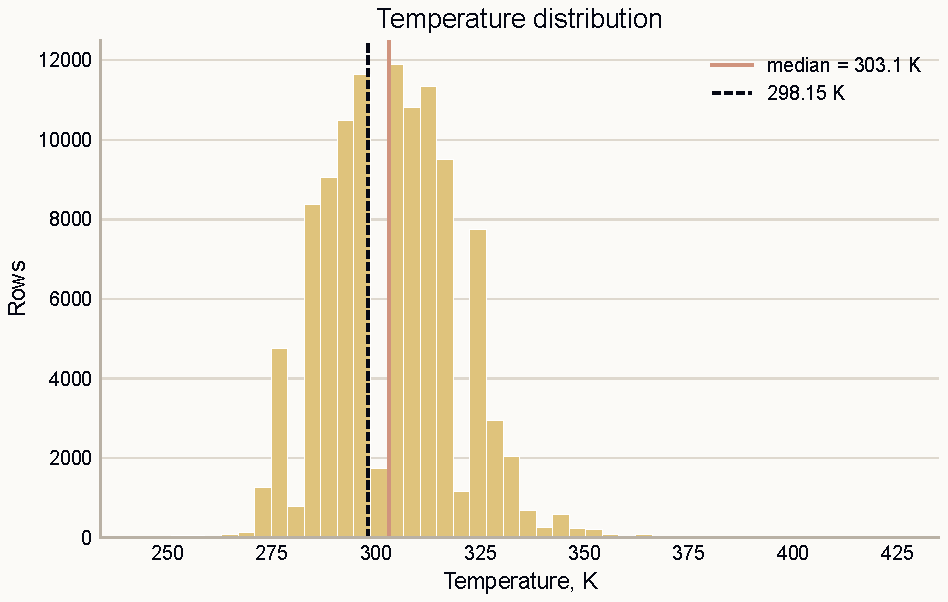
\includegraphics[width=0.70\textwidth]{corpus_temperature_histogram.pdf}
\caption{Распределение температур в корпусе. Большинство измерений сосредоточено около комнатной температуры, поэтому температурная экстраполяция требует отдельного протокола.}
\label{fig:app-corpus-temperature}
\end{figure}

\begin{figure}[!htbp]
\centering
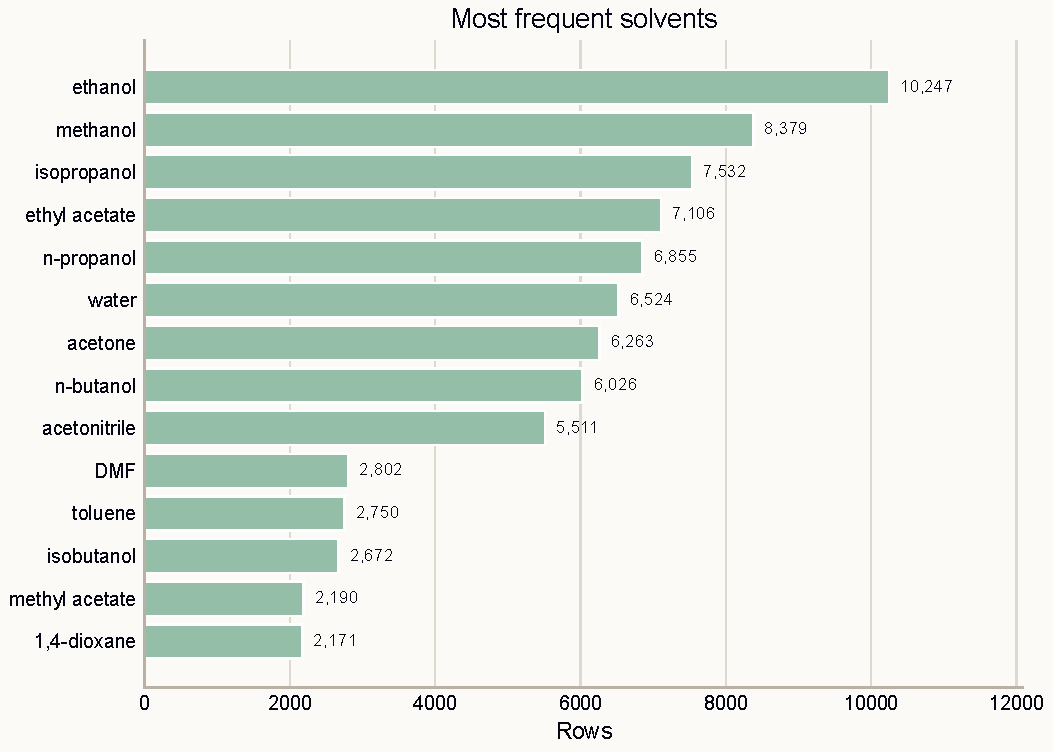
\includegraphics[width=0.76\textwidth]{corpus_solvent_barplot.pdf}
\caption{Наиболее частые растворители. Распределение растворителей неравномерно: часть растворителей представлена тысячами строк, а длинный хвост встречается редко.}
\label{fig:app-corpus-solvents}
\end{figure}

Отдельный аудит происхождения строк показывает, что корпус не сводится к одной-двум публикациям. Сто крупнейших источников дают около $16.4\%$ строк, пятьсот крупнейших --- около $57.3\%$. Это объясняется детальностью поля источника: записи различаются на уровне DOI, статьи или описания набора. Поэтому шум источников нужно учитывать, но удаление одного доминирующего источника не решает задачу.

\begin{figure}[!htbp]
\centering
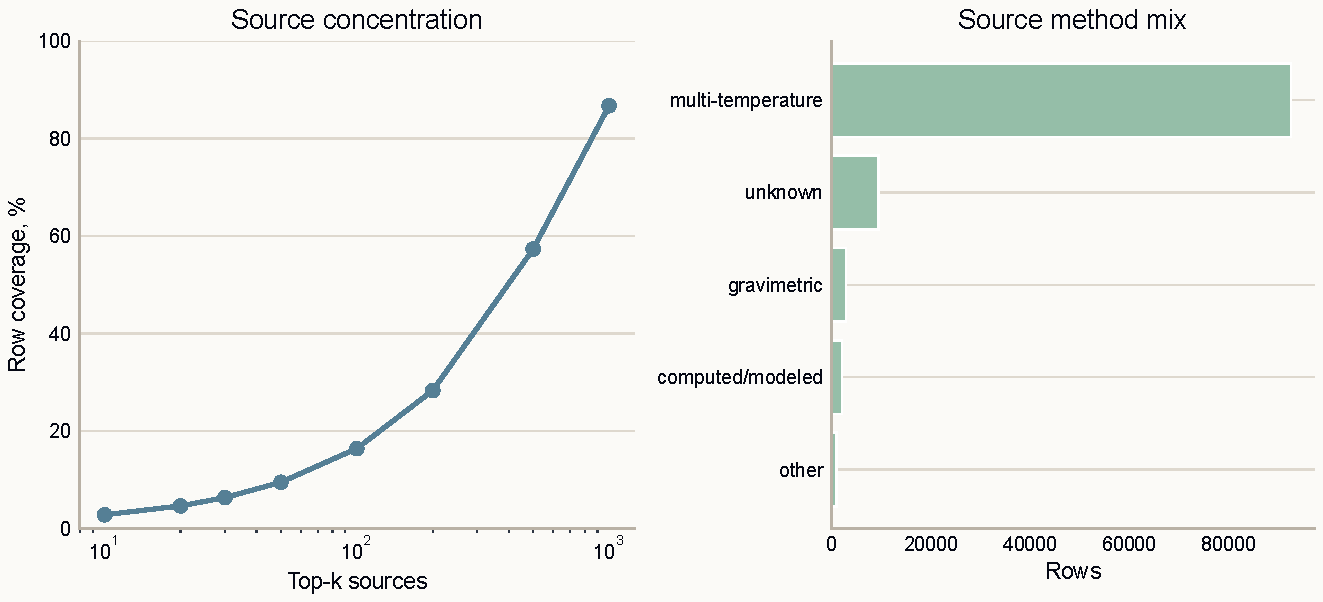
\includegraphics[width=0.92\textwidth]{source_uncertainty_coverage.pdf}
\caption{Аудит происхождения строк. Слева показана концентрация корпуса по крупнейшим источникам, справа --- приближённая смесь типов измерений после эвристической классификации.}
\label{fig:app-source-coverage}
\end{figure}

\begin{figure}[!htbp]
\centering
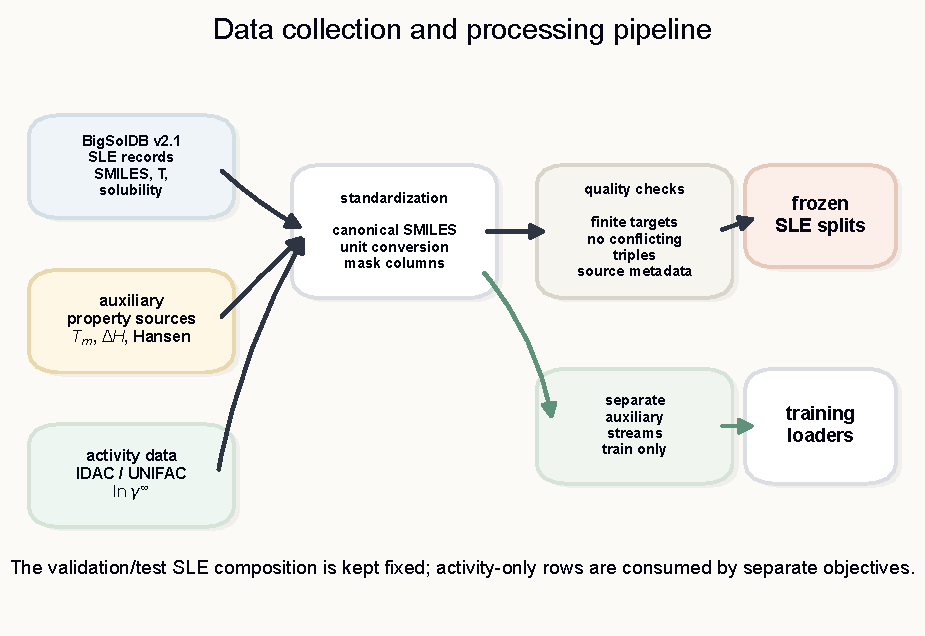
\includegraphics[width=0.96\textwidth]{data_collection_pipeline_schematic.pdf}
\caption{Схема подготовки данных. SLE-строки фиксируют основную задачу растворимости; вспомогательные физические данные подключаются через маски или отдельные обучающие потоки.}
\label{fig:app-data-pipeline}
\end{figure}

\subsection{IDAC и UNIFAC как вспомогательный сигнал активности}

Параметры активности в TGNN-Solv не наблюдаются напрямую. Одна строка растворимости ограничивает сумму кристаллического вклада и вклада активности, но не разделяет их. IDAC-данные закрывают часть этого разрыва: они дают частичный прямой сигнал на предел $\ln\gamma_2^{\infty}$, связанный с теми же NRTL-параметрами.

Стартовый IDAC-корпус содержал $404$ экспериментальные строки, $138$ пар и $9$ DOI. После расширения через NIST ThermoML получено $14\,900$ агрегированных строк, $3\,145$ пар, $136$ растворяемых веществ, $112$ растворителей и $63$ DOI. Конфликтующих агрегированных групп при пороге стандартного отклонения $0.5$ в $\ln\gamma^\infty$ не найдено. Точное пересечение с SLE-парами и SLE-тройками равно $0\%$: нет записей с теми же парой вещество--растворитель и температурной точкой. Утечки целевой растворимости это не создаёт, но остаётся более мягкий вопрос переноса: отдельные молекулы или функциональные классы могут встречаться в обоих источниках и влиять на представления.

\begin{table}[!htbp]
\centering
\caption{Расширение IDAC-корпуса.}
\label{tab:app-idac-expansion}
\small
\begin{tabular}{lrr}
\toprule
Показатель & Стартовый набор & Расширенный набор \\
\midrule
Строки & $404$ & $14\,900$ \\
Уникальные пары & $138$ & $3\,145$ \\
Уникальные растворяемые вещества & --- & $136$ \\
Уникальные растворители & --- & $112$ \\
DOI-источники & $9$ & $63$ \\
Конфликтующие агрегированные группы & --- & $0$ \\
Точное пересечение с SLE-парами & --- & $0\%$ \\
Точное пересечение с SLE-тройками & --- & $0\%$ \\
\bottomrule
\end{tabular}
\end{table}

Важное ограничение этого результата: IDAC-пары не совпадают с SLE-парами. Значит, IDAC не подсказывает ответ для теста. Он проверяет другое предположение: можно ли выучить переносимую функцию активности, которая затем поможет на новых парах. Нужна абляция «с IDAC / без IDAC» при одном и том же SLE-разбиении; без неё польза расширенного IDAC-корпуса остаётся физически мотивированной, но не доказанной.

\begin{figure}[!htbp]
\centering
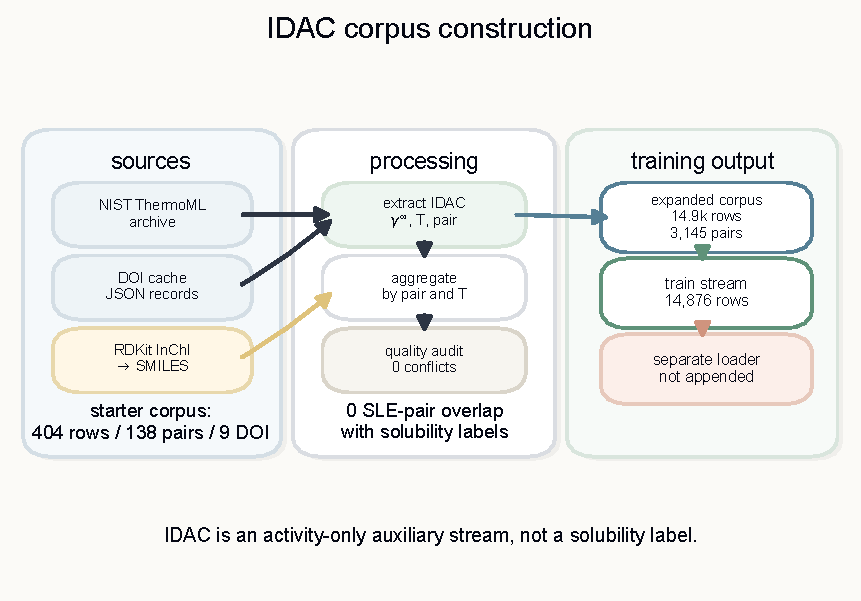
\includegraphics[width=0.94\textwidth]{idac_collection_pipeline_schematic.pdf}
\caption{Схема извлечения IDAC-данных из ThermoML. IDAC-строки остаются отдельным обучающим потоком и не превращаются в псевдостроки растворимости.}
\label{fig:app-idac-pipeline}
\end{figure}

\begin{figure}[!htbp]
\centering
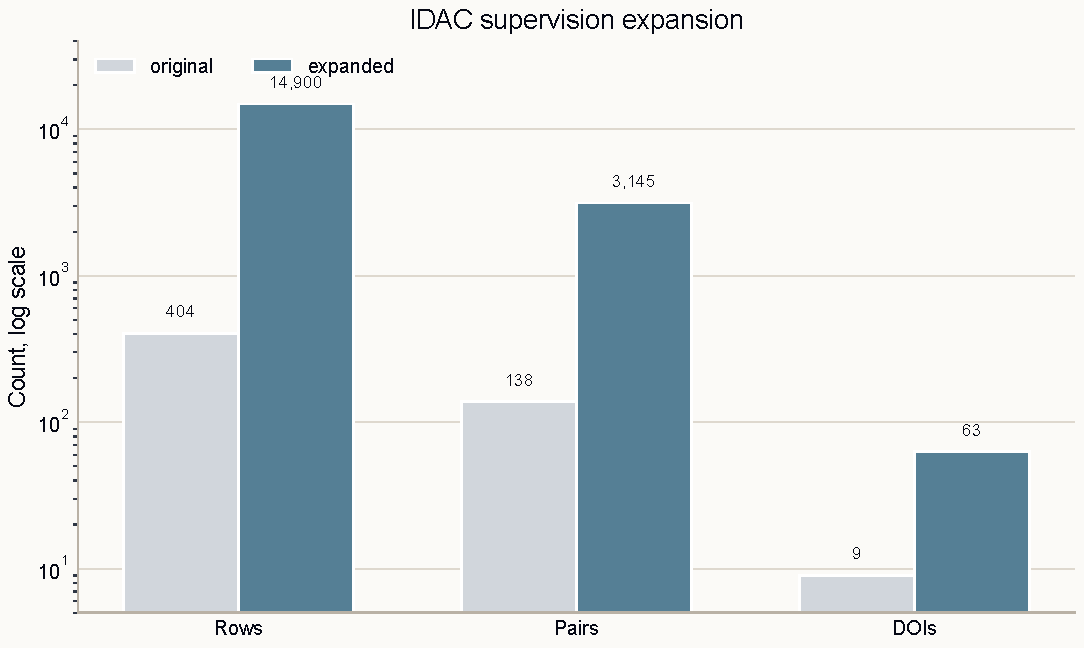
\includegraphics[width=0.76\textwidth]{idac_expansion_bars.pdf}
\caption{Масштаб расширения IDAC-разметки относительно стартового набора.}
\label{fig:app-idac-bars}
\end{figure}

UNIFAC-псевдометки используются осторожнее. Они дают слабый ориентир для $\ln\gamma_2^\infty$, но покрытие каркасного теста ограничено: около $8.6\%$ строк и $10.9\%$ уникальных пар. UNIFAC здесь работает как слабый физический приор там, где функциональные группы распознаны, а не как самостоятельное решение для новых каркасов.

\subsection{Открытый путь для кристаллических данных}

Для кристаллической части задачи теперь выделен отдельный воспроизводимый контур, чтобы не опираться на ручные подстановки отдельных веществ. Он состоит из двух шагов: \code{scripts/data/extract_crystal_from_thermoml.py} извлекает чистокомпонентные $\Tm$ и $\dHfus$ из локального кэша NIST ThermoML JSON, а \code{scripts/data/build_open_crystal_artifact.py} объединяет эти значения с уже используемыми открытыми источниками и сохраняет явный приоритет источников.

На текущем локальном кэше из $3721$ ThermoML JSON получено $1679$ сырых кристаллических измерений, $701$ агрегированное вещество с $\Tm$ и $473$ вещества с $\dHfus$; все $473$ энтальпии приходят только из DOI-групп, где для того же вещества есть и точка плавления. Это важно: кристаллический путь расширяется не произвольными переходами фаз, а тем подмножеством ThermoML, где хотя бы минимально прослеживается совместная кристаллическая информация.

\begin{table}[!htbp]
\centering
\caption{Открытый кристаллический артефакт и прирост покрытия относительно текущего канонического корпуса.}
\label{tab:app-open-crystal}
\small
\begin{tabular}{lr}
\toprule
Показатель & Значение \\
\midrule
Сырые ThermoML-измерения $\Tm/\dHfus$ & $1679$ \\
ThermoML-вещества с $\Tm$ & $701$ \\
ThermoML-вещества с $\dHfus$ & $473$ \\
Итоговый open-артефакт: вещества с $\Tm$ & $19\,436$ \\
Итоговый open-артефакт: вещества с $\dHfus$ & $495$ \\
Итоговый open-артефакт: вещества с $\Tm+\dHfus$ & $495$ \\
Supervised строки с $\Tm+\dHfus$: было $\to$ стало & $1080 \to 14\,910$ \\
Такие строки в validation: было $\to$ стало & $0 \to 288$ \\
Такие строки в test: было $\to$ стало & $0 \to 221$ \\
Уникальные пары с $\Tm+\dHfus$: было $\to$ стало & $146 \to 1497$ \\
\bottomrule
\end{tabular}
\end{table}

Явный приоритет источников выбран консервативно. Для $\Tm$ используется порядок ``curated NIST/WebBook $\rightarrow$ ThermoML $\rightarrow$ Bradley'', а для $\dHfus$ --- ``curated NIST/WebBook $\rightarrow$ ThermoML''. На пересечении curated и ThermoML точки плавления согласуются хорошо: $13$ перекрывающихся веществ дают медианное абсолютное расхождение всего $0.275\,\mathrm K$. Для $\dHfus$ перекрытие меньше и шумнее: на $9$ веществах медианное расхождение равно $930\,\mathrm{J/mol}$, а хвост длинный из-за разных фазовых форм и неоднозначного поля transition/fusion. Самый жёсткий вывод относится к Bradley: на $307$ веществах, где есть и ThermoML, медианное абсолютное расхождение по $\Tm$ равно $273.45\,\mathrm K$. Поэтому Bradley полезен как широкий, но низкоприоритетный источник покрытия, а не как опорная истина там, где уже есть ThermoML.

Этот open-артефакт пока остаётся отдельным sidecar-ресурсом, а не молчаливой заменой канонических \code{train.csv}/\code{val.csv}/\code{test.csv}. Причина проста: прирост покрытия велик, но он меняет режим прямой кристаллической супервизии и требует отдельного решения, когда именно такой источник должен становиться частью поддерживаемого benchmark-контракта.

\subsection{Режимы оценки и почему главный тест труден}

В проекте используются разные разбиения, потому что они отвечают на разные научные вопросы. Случайное разбиение строк проверяет почти интерполяцию: одна и та же пара часто видна в обучении и тесте при другой температуре. Разбиение по новым каркасам намного строже: модель должна переноситься на новые структурные классы растворяемых веществ.

\begin{table}[!htbp]
\centering
\caption{Смысл основных режимов оценки.}
\label{tab:app-evaluation-regimes}
\small
\begin{tabularx}{\textwidth}{P{0.25\textwidth}Y}
\toprule
Разбиение & Что проверяет \\
\midrule
Случайные строки & Интерполяционный режим с сильным пересечением пар между обучением и тестом \\
Случайные пары & Новая пара, но оба компонента часто уже встречались по отдельности \\
Новый растворитель & Перенос на растворитель, отсутствующий в обучении \\
Новое вещество & Перенос на новый растворяемый компонент \\
Новый каркас & Перенос на новый структурный класс растворяемого вещества \\
Та же пара, новая температура & Умение использовать физическую форму зависимости от температуры \\
\bottomrule
\end{tabularx}
\end{table}

\begin{figure}[!htbp]
\centering
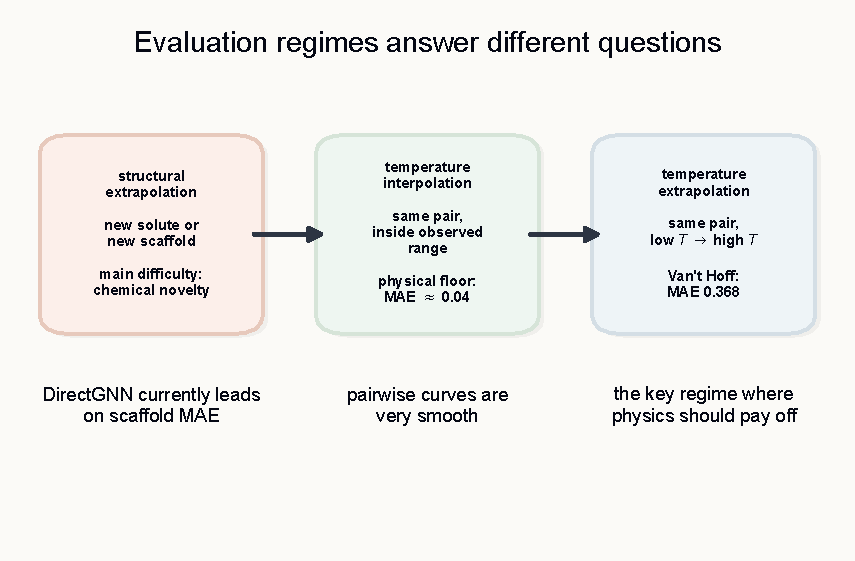
\includegraphics[width=0.92\textwidth]{evaluation_regimes_schematic.pdf}
\caption{Разные режимы оценки проверяют разные виды обобщения. Главный вывод по новым каркасам нельзя заменять результатом на случайных строках.}
\label{fig:app-evaluation-regimes}
\end{figure}

Сравнение на случайном лесе показывает масштаб различий между разбиениями. Случайные строки дают почти идеальный результат, потому что тест близок к обучению. Новые вещества и новые каркасы резко труднее. Это подтверждает, что основной барьер --- перенос на новую химию растворяемого вещества.

\begin{table}[!htbp]
\centering
\caption{Сложность разных разбиений по ориентиру случайного леса.}
\label{tab:app-split-difficulty}
\small
\begin{tabular}{lrrl}
\toprule
Разбиение & $\mae$ & $\Rtwo$ & Интерпретация \\
\midrule
Случайные строки & 0.166 & 0.987 & слишком лёгкий режим \\
Случайные пары & 0.783 & 0.806 & новые пары, но знакомые компоненты \\
Новый растворитель & 0.732 & 0.735 & перенос по растворителю относительно легче \\
Новое вещество & 1.642 & 0.420 & трудный перенос на новое вещество \\
Новый каркас & 1.703 & 0.462 & новый каркас и смещение распределения \\
\bottomrule
\end{tabular}
\end{table}

\subsection{Методы сравнения и смысл физического пути}

Сравнение TGNN-Solv и DirectGNN имеет смысл только потому, что у них общий графовый блок. DirectGNN проверяет, насколько хорошо та же молекулярная обработка решает задачу без физического слоя. Случайный лес показывает силу дескрипторного подхода без нейросетевого графа. SolProp и FastSolv нужны как внешние ориентиры, но их статус различен: SolProp в этом отчёте переобучен в том же контракте данных, а FastSolv потребовал отдельного исправления преобразований единиц.

\begin{table}[!htbp]
\centering
\caption{Классы методов, с которыми сопоставляется TGNN-Solv.}
\label{tab:app-method-classes}
\small
\begin{tabularx}{\textwidth}{P{0.20\textwidth}P{0.20\textwidth}Y}
\toprule
Класс методов & Примеры & Ограничение для этой задачи \\
\midrule
Дескрипторные модели & GSE, QSPR, случайный лес & Не разделяют вклад кристалла и раствора; температура обычно входит как обычный признак \\
Групповые модели активности & UNIFAC, Modified UNIFAC & Зависят от покрытия функциональных групп и плохо работают вне известных групп \\
Модели избыточной энергии & NRTL, Wilson, UNIQUAC & Требуют параметров активности, которые трудно идентифицировать только из SLE \\
Графовые нейронные сети & MPNN, GAT, Chemprop-подобные модели & Обычно дают один итоговый скаляр без физической декомпозиции \\
Внешние модели растворимости & SolProp, FastSolv & Имеют собственные протоколы; для честного сравнения требуют адаптеров и проверки единиц \\
\bottomrule
\end{tabularx}
\end{table}

Выбор NRTL не означает, что Wilson или UNIQUAC «неправильны»~\cite{wilson1964,abrams1975}. NRTL выбран как практичный компромисс: она достаточно гибкая для бинарной неидеальности, допускает асимметричные взаимодействия и естественно даёт $\gamma_i(x,T)$ для SLE. Wilson и UNIQUAC остаются корректными альтернативами для отдельных абляций, но требуют собственной проверки области применимости и параметризации.

\subsection{Архитектура и обучение}

Архитектура состоит из нескольких уровней. Графовый блок строит представления растворяемого вещества и растворителя, затем формируется парное представление, после чего TGNN-Solv разветвляется на кристаллический путь, NRTL-путь, решатель и ограниченную остаточную поправку. DirectGNN использует тот же входной и парный блок, но заменяет всю физическую часть прямым предсказанием $\ln x_2$.

Ограниченная остаточная поправка является компромиссом. Она нужна, чтобы модель могла исправить систематический промах физического расчёта, не превращаясь в полностью прямую регрессию. Но её вклад нельзя автоматически считать физически интерпретируемым. Если поправка в основном меняет параметры активности на строках с ошибочным кристаллическим уровнем, она численно маскирует одну ошибку другой. Поэтому для следующего запуска требуется отдельный журнал величин поправки по $\Tm$, $\dHfus$, $\Delta C_p^{\mathrm{fus}}$, $\tau_{12}$ и $\tau_{21}$.

\begin{figure}[!htbp]
\centering
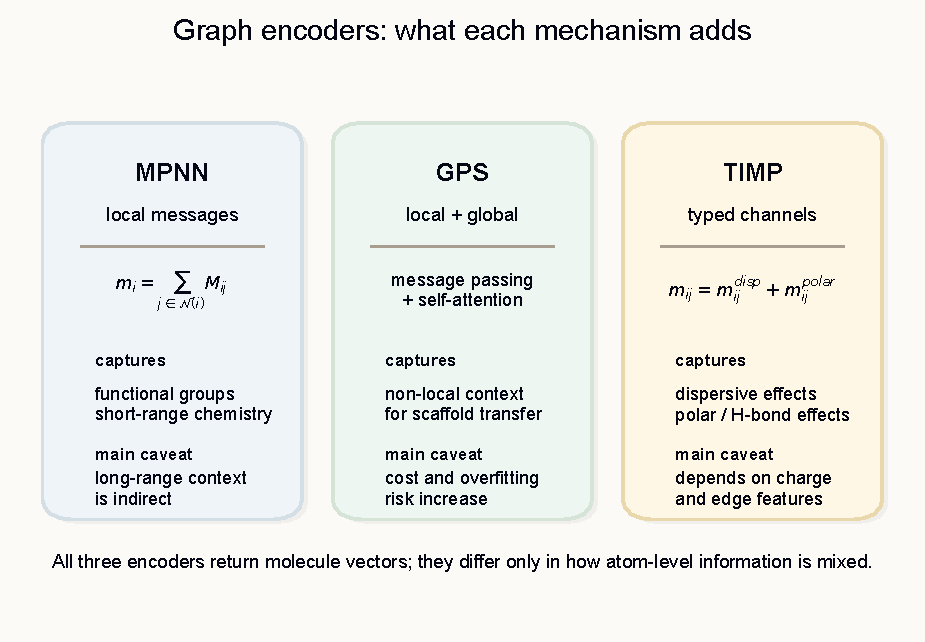
\includegraphics[width=0.92\textwidth]{graph_mechanisms_schematic.pdf}
\caption{Графовые механизмы, используемые в моделях. Они отвечают за перенос молекулярной структуры в векторные представления, но сами по себе не задают физику SLE.}
\label{fig:app-graph-mechanisms}
\end{figure}

\begin{figure}[!htbp]
\centering
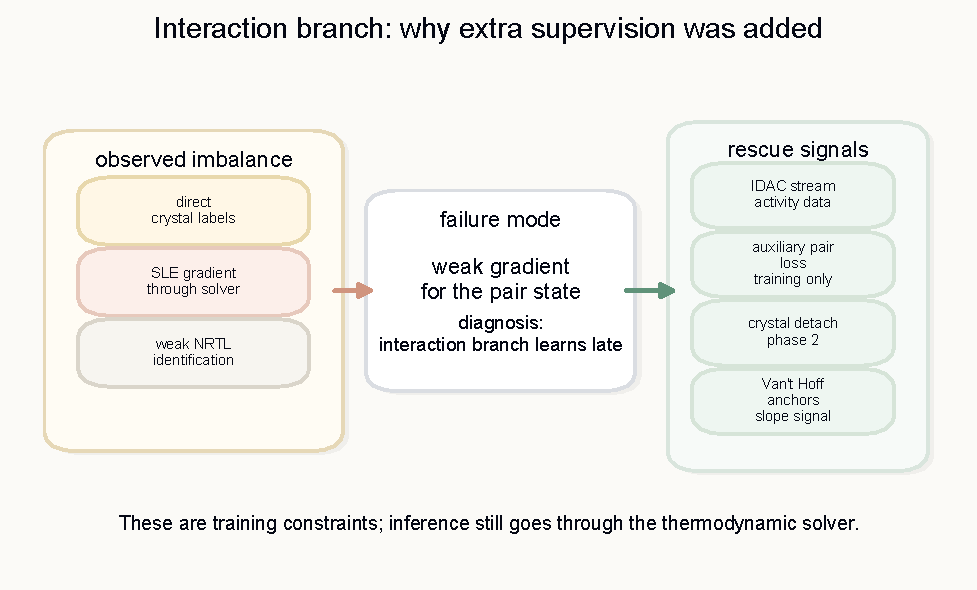
\includegraphics[width=0.92\textwidth]{interaction_rescue_schematic.pdf}
\caption{Идея усиления парного сигнала: кристаллические свойства зависят от одиночной молекулы, а растворимость требует совместимости пары вещество--растворитель.}
\label{fig:app-interaction-rescue}
\end{figure}

Отдельная диагностика потока градиентов уточнила, что проблема не сводится к отсутствию градиента в модели вообще. Энкодер TGNN-Solv получал заметный сигнал, но не тот путь, который нужен для активности раствора: сильнее обучалась кристаллическая ветвь одиночной молекулы, а слой перекрёстного внимания, формирующий совместимость вещества и растворителя, получал слабый сигнал.

\begin{center}
\small
\begin{tabularx}{0.86\textwidth}{Y C{2.1cm} C{2.1cm} C{2.1cm}}
\toprule
Блок & TGNN-Solv & DirectGNN & Отношение \\
\midrule
Энкодер, слой 0 & $0.037$ & $0.008$ & $4.9\times$ \\
Попарное перекрёстное внимание & $0.0007$ & $0.023$ & $0.03\times$ \\
Голова кристалла / прямая голова & $1.25$ & $0.78$ & $1.6\times$ \\
Адаптер растворителя & $6\cdot10^{-6}$ & $2\cdot10^{-4}$ & $0.03\times$ \\
\bottomrule
\end{tabularx}
\end{center}

Это диагностический прогон, а не финальный результат качества. Он показывает место, где физический путь теряет обучающий сигнал. Если парное представление не обучается, NRTL-голова не получает химически полезных признаков контакта, даже при математически корректных SLE-решателе и неявном дифференцировании.

Исправление, проверенное для этого механизма, состоит из двух частей. Первая --- вспомогательная прямая ветка от парного вектора $\mathbf g_{\mathrm{pair}}$ к $\ln x_2$ с малым весом только во время обучения:
\begin{equation*}
    \mathcal L_{\mathrm{aux\ pair}}
    =
    \rho\!\left(f_{\mathrm{aux}}(\mathbf g_{\mathrm{pair}})-\ln x_2^{\mathrm{exp}}\right).
\end{equation*}
Она не используется как финальный прогноз и не должна обходить SLE-путь; её задача --- дать перекрёстному вниманию прямой обучающий сигнал. Вторая --- защитить общий энкодер от доминирования кристаллической головы во второй фазе, например подавая в кристаллическую ветвь вектор $\operatorname{sg}(\mathbf g_{\mathrm{sol}})$, отсоединённый от градиента.

Короткая проверка на $50$ шагах показала именно исправление механики градиента: после вспомогательной ветки норма градиента попарного внимания стала $0.0377$ против $0.0381$ у DirectGNN. Норма градиента блока взаимодействия сравнялась с соответствующей нормой в прямой модели. Проверка пока говорит только о потоке градиента; влияние на MAE, разброс $\tau$ и вклад $\ln\gamma_2$ нужно измерять при одинаковом бюджете обучения.

Сама трёхфазная схема тоже должна рассматриваться как гипотеза, а не как окончательно правильный протокол. Она стабилизирует решатель, но может усилить дисбаланс между кристаллическим и парным сигналом: кристаллическая ветвь получает прямую задачу раньше, а активностная ветвь включается позже и чаще учит остаток. Альтернативный протокол для проверки --- совместное обучение с малым начальным весом SLE-потери и плавным ростом этого веса, без полной изоляции ветвей на раннем этапе.

\begin{figure}[!htbp]
\centering
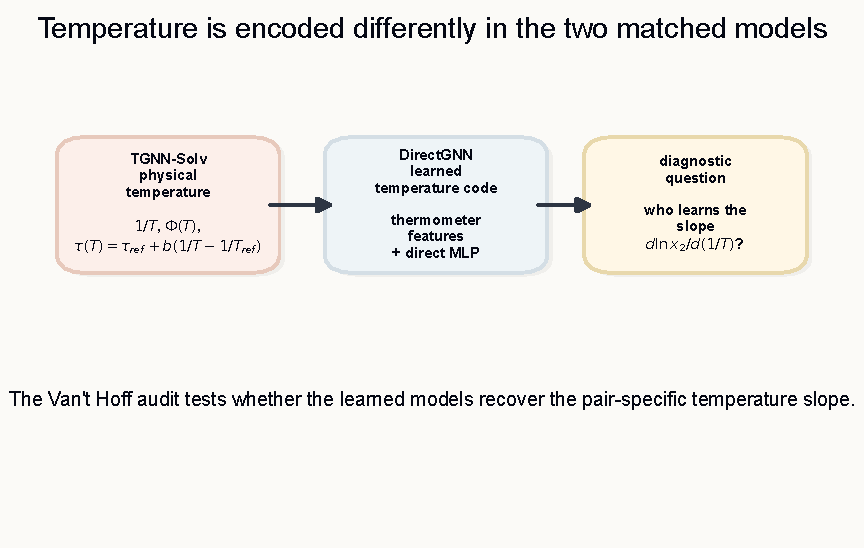
\includegraphics[width=0.82\textwidth]{temperature_encoding_schematic.pdf}
\caption{Температура входит в модель не как произвольная колонка таблицы, а как часть физического расчёта и как кодировка для прямой модели.}
\label{fig:app-temperature-encoding}
\end{figure}

Обучение физической модели проводится поэтапно. Сначала графовый блок и физические головы получают более простой сигнал, затем включается полный SLE-путь, после чего выполняется тонкая настройка с меньшим шагом. Эта схема нужна не из-за эстетики, а из-за численной обусловленности: случайные NRTL-параметры в начале обучения могут давать плохие градиенты через решатель.

\begin{figure}[!htbp]
\centering
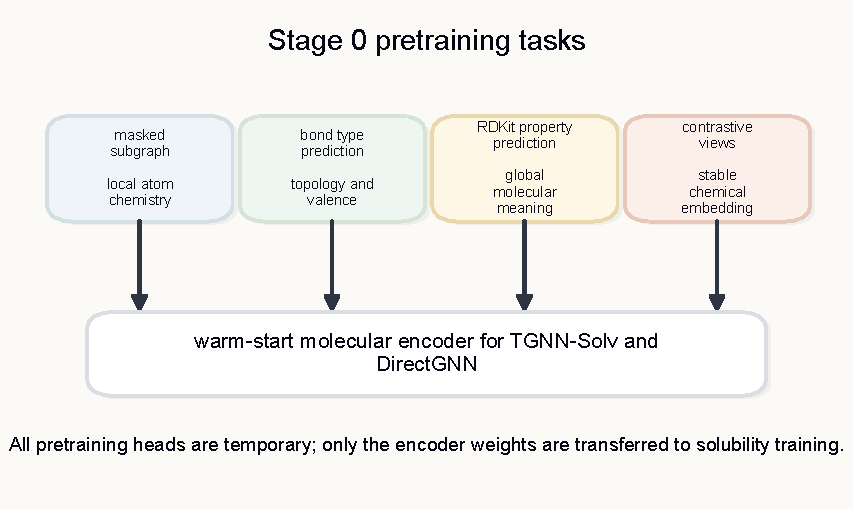
\includegraphics[width=0.90\textwidth]{pretraining_tasks_schematic.pdf}
\caption{Предобучение графового блока на молекулярных задачах. Оно улучшает химическое представление одиночной молекулы, но не заменяет обучение парной совместимости.}
\label{fig:app-pretraining-tasks}
\end{figure}

\begin{figure}[!htbp]
\centering
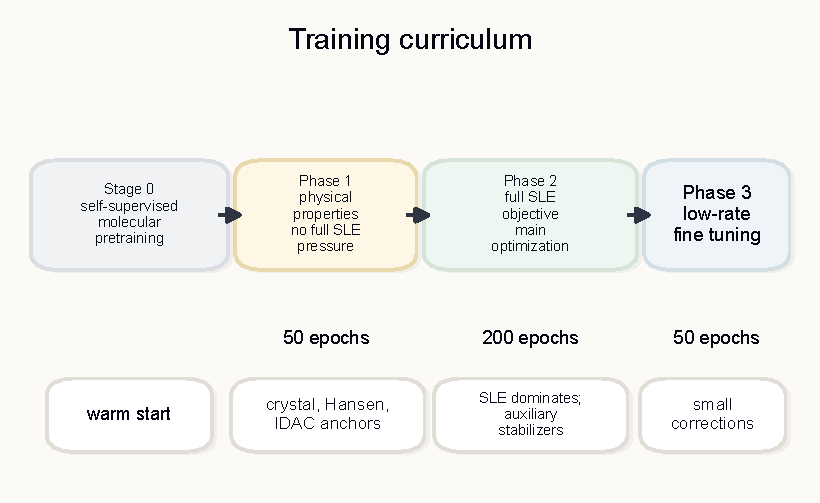
\includegraphics[width=0.94\textwidth]{training_curriculum_schematic.pdf}
\caption{Трёхфазная схема обучения TGNN-Solv. Решатель получает физически разумные входы до того, как становится главным источником градиента.}
\label{fig:app-training-curriculum}
\end{figure}

\begin{figure}[!htbp]
\centering
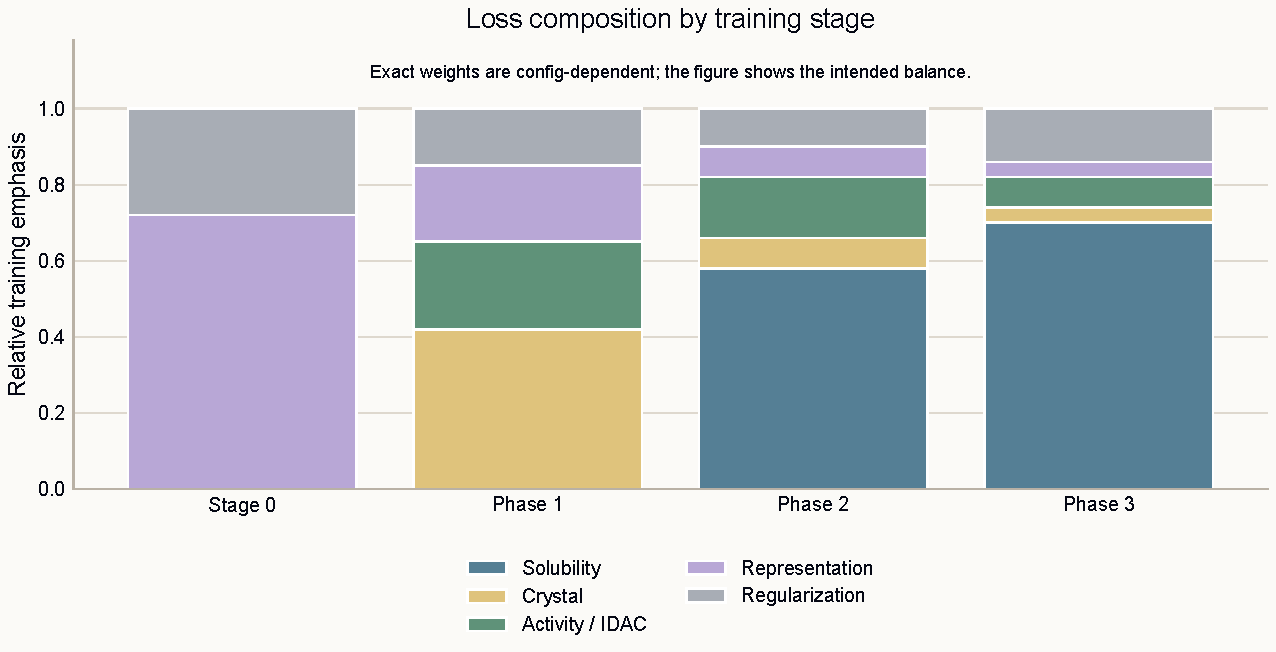
\includegraphics[width=0.86\textwidth]{loss_components_schematic.pdf}
\caption{Состав функции ошибки. Физические члены стабилизируют промежуточные величины, но не должны вытеснять главную ошибку по растворимости.}
\label{fig:app-loss-components}
\end{figure}

\begin{figure}[!htbp]
\centering
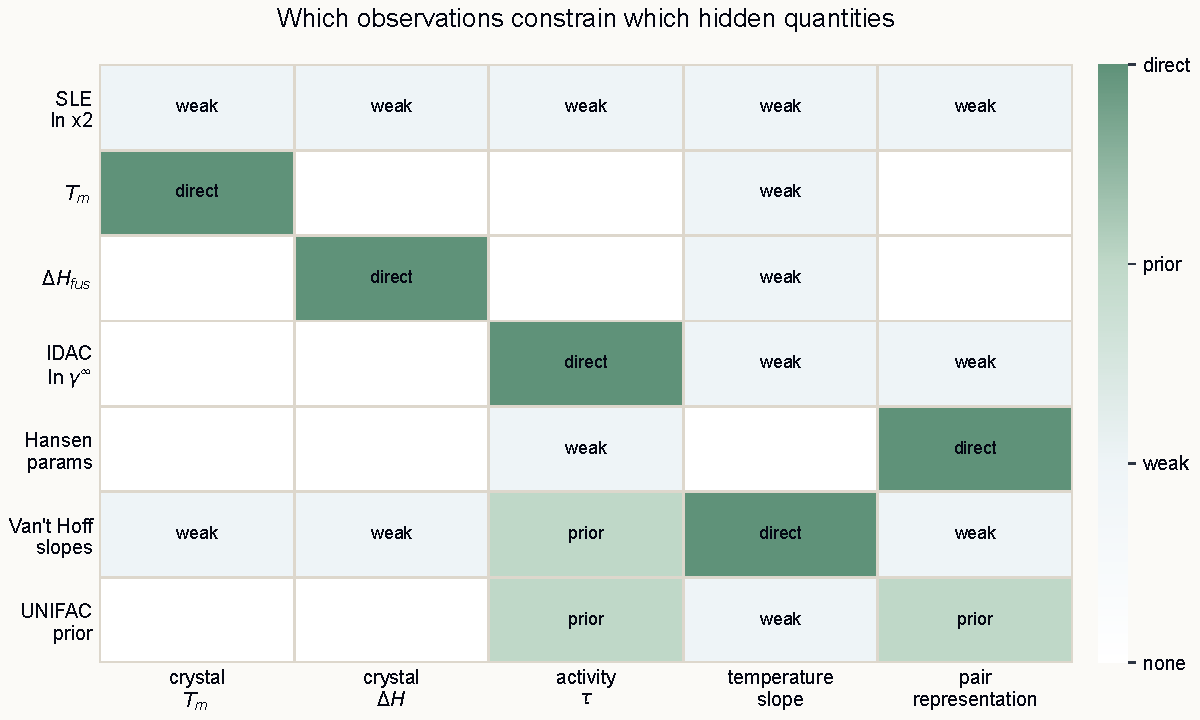
\includegraphics[width=0.90\textwidth]{supervision_matrix.pdf}
\caption{Какие наблюдения ограничивают скрытые величины модели. Одна SLE-метка видит сумму кристаллического вклада и активности, поэтому отдельные сигналы на $T_m$, $\Delta H_{\mathrm{fus}}$ и $\ln\gamma^\infty$ необходимы.}
\label{fig:app-supervision-matrix}
\end{figure}

\subsection{Основные результаты и структура ошибки}

Главная таблица показывает небольшой проигрыш TGNN-Solv прямой графовой модели на новых каркасах. Однако построчная и парная диагностика показывают, что это не равномерное ухудшение. TGNN-Solv выигрывает примерно на $46\%$ строк и пар, но проигрывает из-за более крупных локальных ошибок.

\begin{table}[!htbp]
\centering
\caption{Основной тест по новым молекулярным каркасам.}
\label{tab:app-scaffold-main}
\small
\begin{tabularx}{\textwidth}{P{0.30\textwidth}rrY}
\toprule
Модель & $\mae$ & $\Rtwo$ & Статус \\
\midrule
DirectGNN & 1.652 & 0.478 & лучшая средняя ошибка в этом запуске \\
Случайный лес, гибридные признаки & 1.722 & 0.449 & сильная контрольная модель \\
TGNN-Solv & 1.741 & 0.438 & физический путь в данной реализации уступает \\
\bottomrule
\end{tabularx}
\end{table}

\begin{figure}[!htbp]
\centering
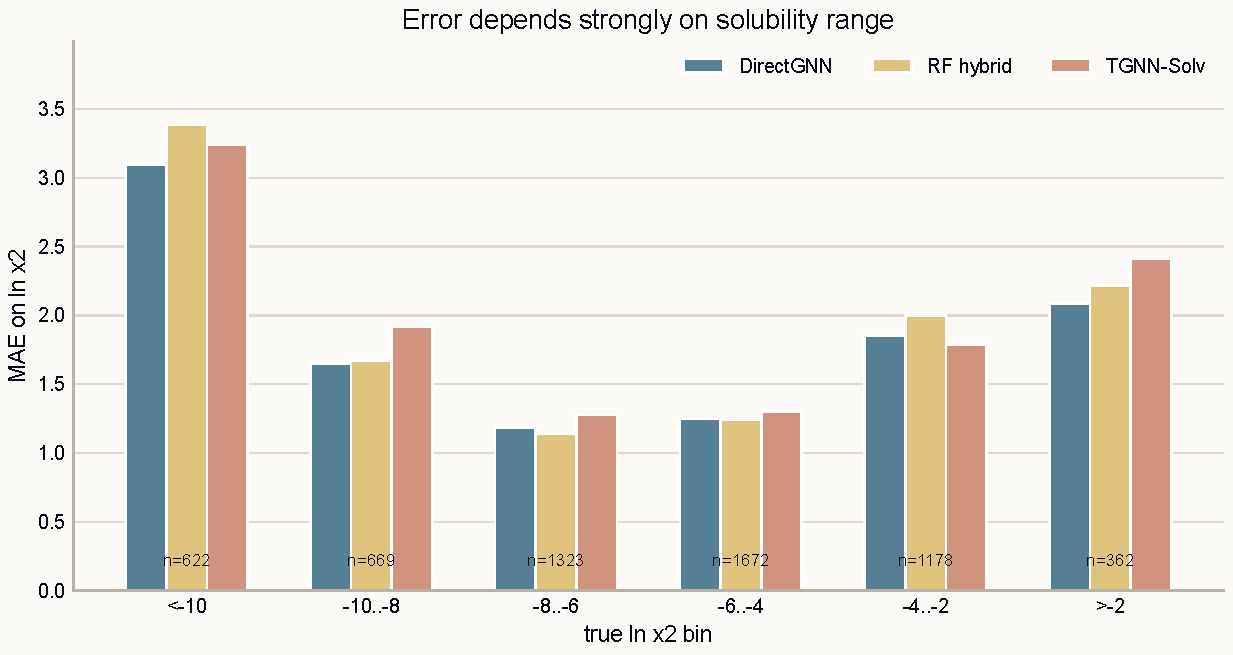
\includegraphics[width=0.88\textwidth]{prediction_slice_lnx2_bin_mae.pdf}
\caption{Ошибка как функция истинной растворимости. Левый хвост очень плохо растворимых систем является одним из главных источников ошибки.}
\label{fig:app-lnx2-bin-mae}
\end{figure}

\begin{figure}[!htbp]
\centering
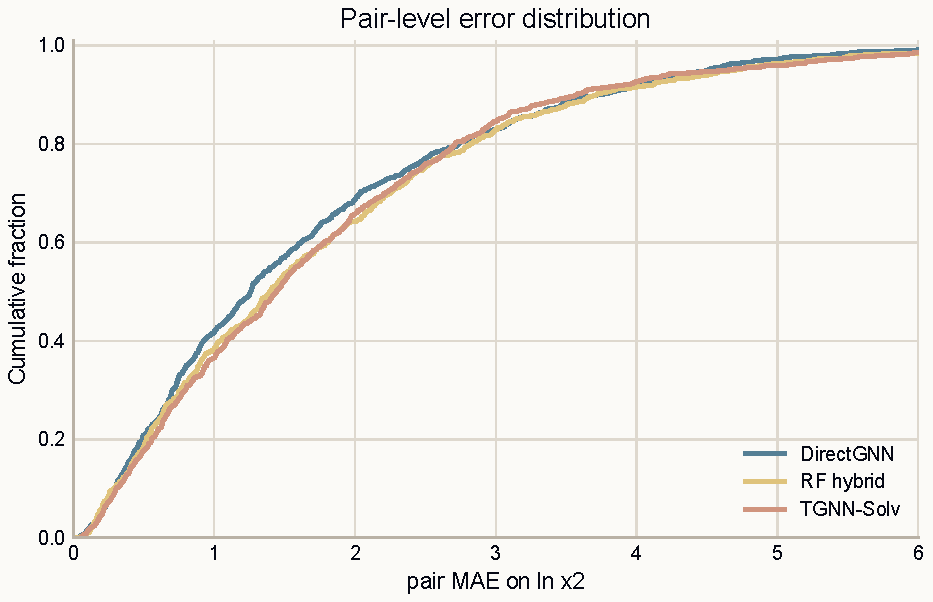
\includegraphics[width=0.64\textwidth]{prediction_slice_pair_mae_cdf.pdf}
\caption{Распределение парных ошибок. Близкая средняя MAE может скрывать разную долю тяжёлых ошибок.}
\label{fig:app-pair-mae-cdf}
\end{figure}

\begin{figure}[!htbp]
\centering
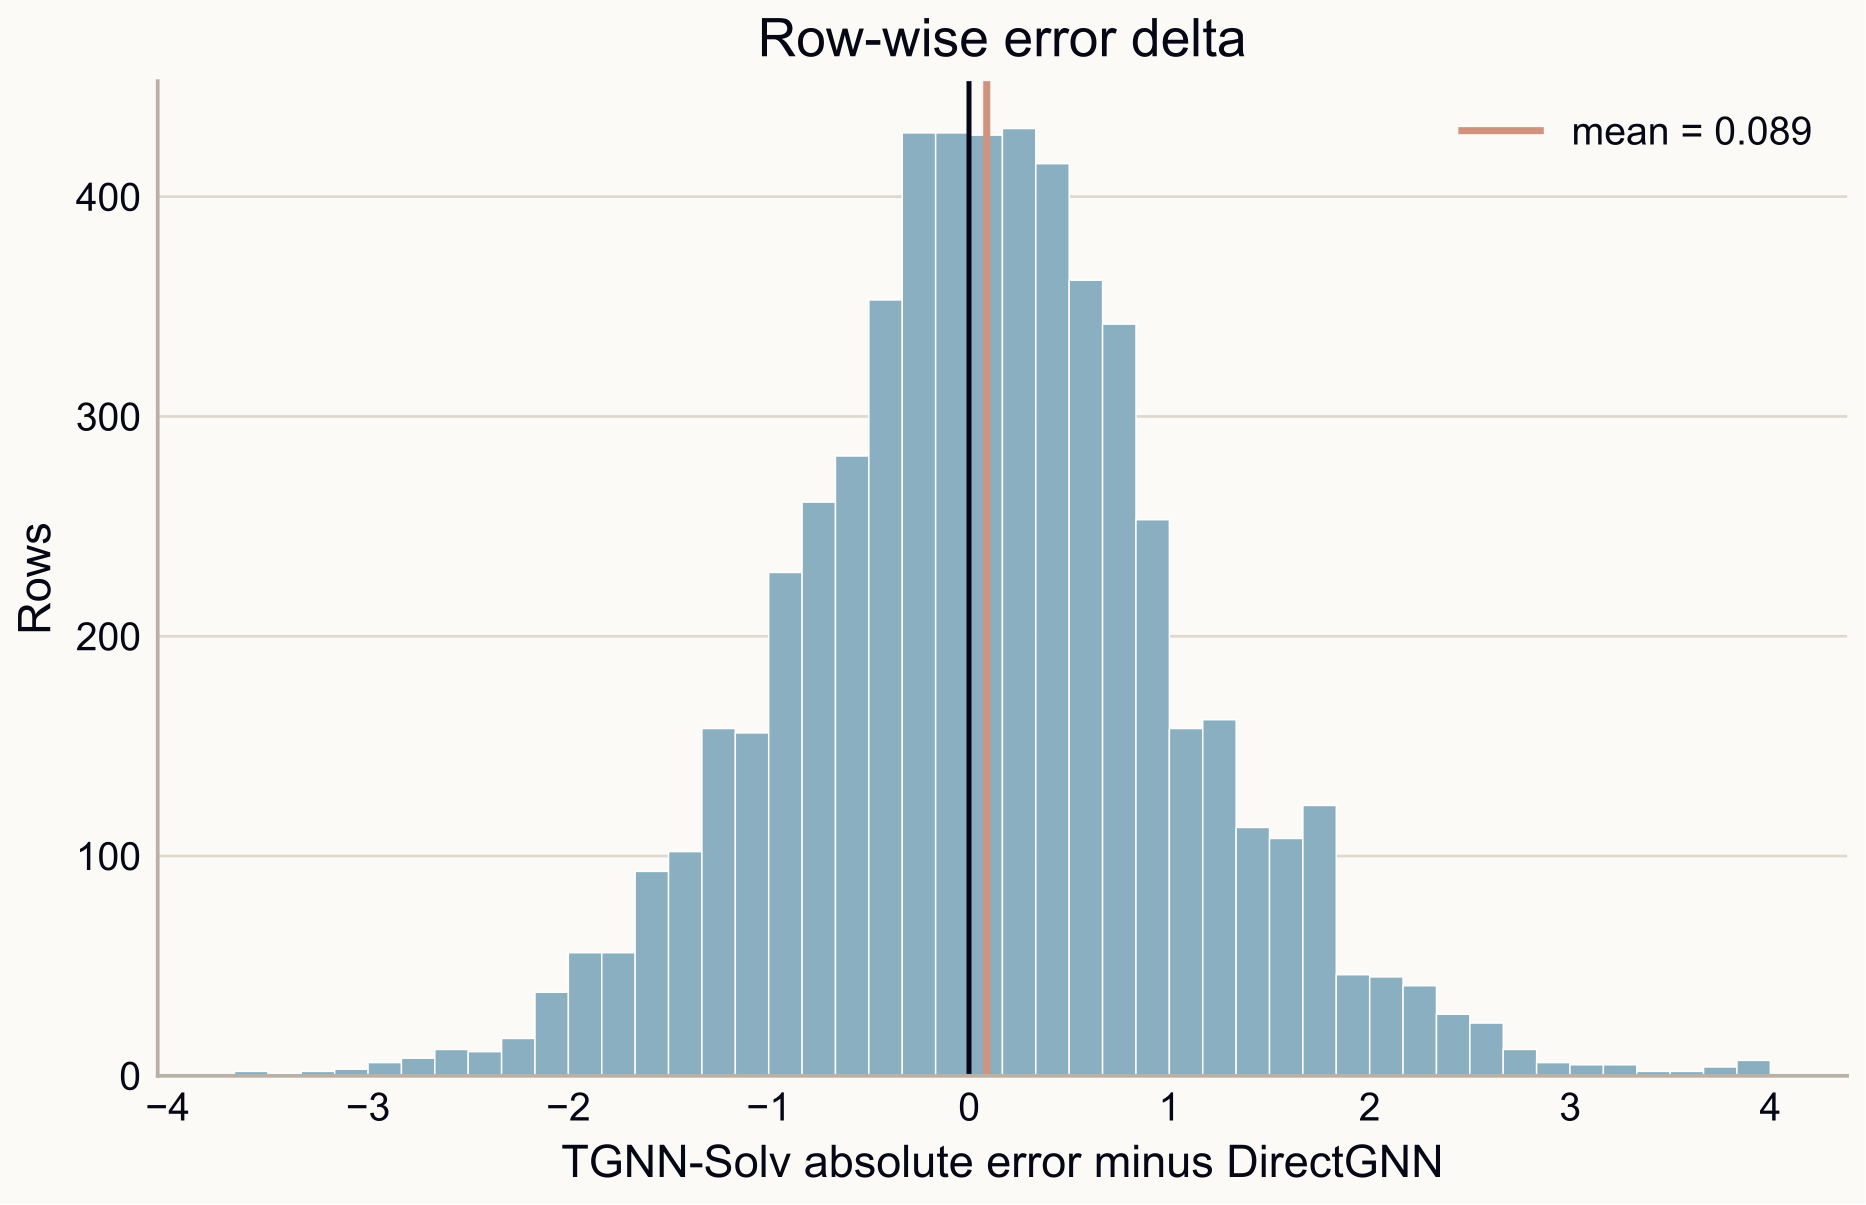
\includegraphics[width=0.64\textwidth]{prediction_slice_paired_deltas_raster.png}
\caption{Построчное сравнение TGNN-Solv и DirectGNN. Физическая модель выигрывает на заметной доле строк, но проигрывает по средней ошибке.}
\label{fig:app-paired-deltas}
\end{figure}

Значение $\Rtwo=0.478$ у лучшей модели в этом сравнении также нужно читать честно: на новых каркасах объясняется меньше половины дисперсии. Это не сбой инфраструктуры, но и не зрелое качество для промышленного прогноза. Результат следует формулировать как промежуточный исследовательский итог, а не как завершённое доказательство преимущества физической модели.

\subsection{Зарядовые системы, дельфинидин и постановочные риски}

Аудит трудных систем классифицирует строки по формальному заряду, числу фрагментов, явной соли, цвиттер-ионности и грубому режиму диэлектрической проницаемости растворителя. Такой разбор нужен, потому что за словом «заряженная система» скрываются разные физические режимы. Явная соль в ацетоне или этаноле может вести себя как контактная ионная пара; соль в воде уже ближе к электролитной постановке.

\begin{figure}[!htbp]
\centering
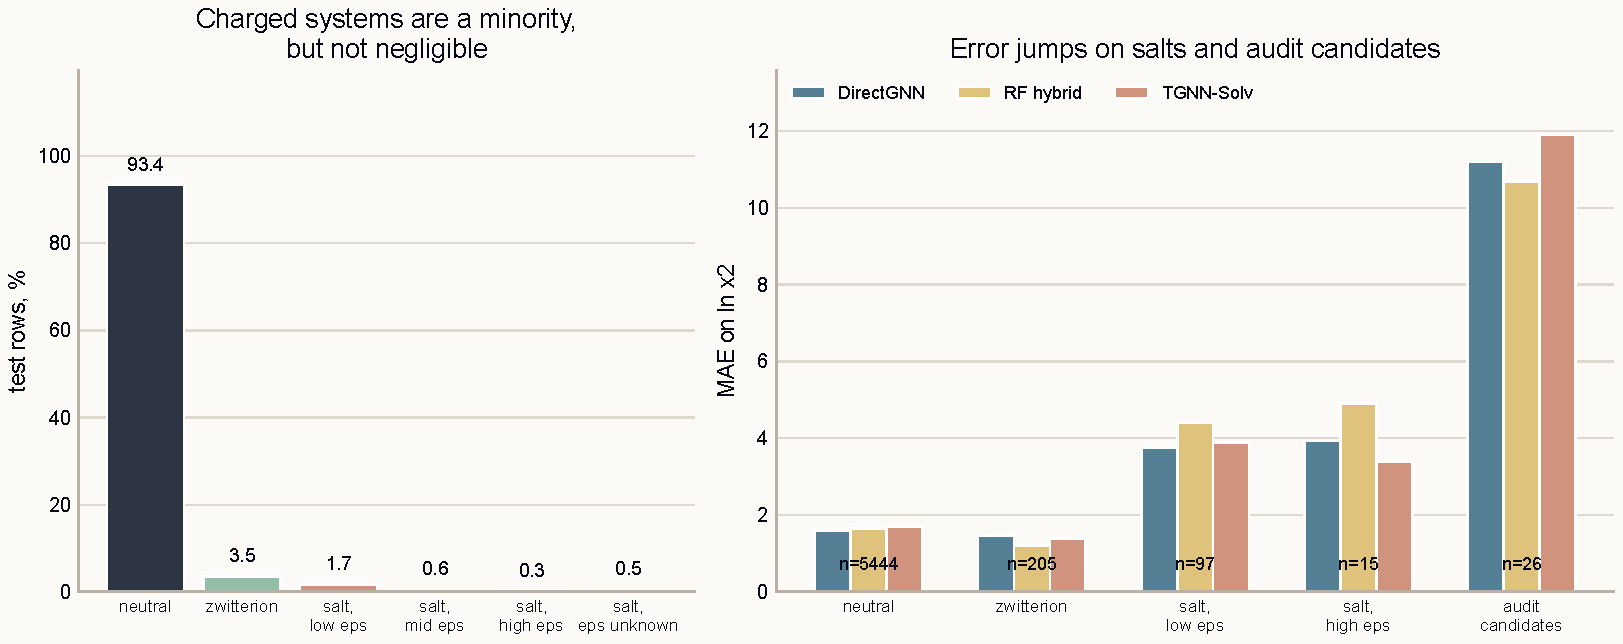
\includegraphics[width=0.96\textwidth]{difficult_systems_audit_summary.pdf}
\caption{Аудит трудных систем на каркасном тесте. Зарядовые системы являются меньшинством, но ошибка на них заметно выше средней.}
\label{fig:app-difficult-systems}
\end{figure}

В основном тесте $6.6\%$ строк имеют формальный заряд, $3.6\%$ являются явными солями, $3.5\%$ --- цвиттер-ионами. Кандидаты на контактные ионные пары в низкодиэлектрических растворителях составляют $3.0\%$ тестовых строк, а кандидаты на настоящую диссоциацию в высокодиэлектрических растворителях --- $0.9\%$. На нейтральных строках DirectGNN имеет $\mae=1.604$, TGNN-Solv --- $1.701$; на зарядовых строках ошибки возрастают до $2.337$ и $2.309$ соответственно.

Особый пример --- дельфинидин-хлорид. В тесте есть $40$ строк: ацетон, этанол, метанол и вода по $10$ температурных точек. Источник описывает чистые растворители~\cite{kumoro2010}; гипотеза о подкисленной смеси для этих строк не подтверждается. Температурные ряды согласованы: растворимость монотонно растёт с температурой, а аппроксимация Вант-Гоффа имеет $R^2>0.991$. В обработанных строках при этом нет экспериментальных $\Tm$ и $\dHfus$. Решатель получает кристаллический вклад из предсказаний кристаллической ветви, а не из экспериментального оракула. Для дельфинидина нельзя корректно посчитать требуемую активность через известный кристаллический вклад. Наиболее осторожная интерпретация: система указывает на проблему кристаллического уровня и представления солевой формы, но без эксперимента с надёжными кристаллическими параметрами нельзя полностью исключить вклад неверной модели активности. Кроме того, флавилиевые соли химически чувствительны к равновесиям форм; если в растворе присутствует смесь флавилиевой, гидратной или другой формы, бинарное SLE-уравнение для одного вещества становится эффективным приближением, а не полной физической постановкой.

\begin{figure}[!htbp]
\centering
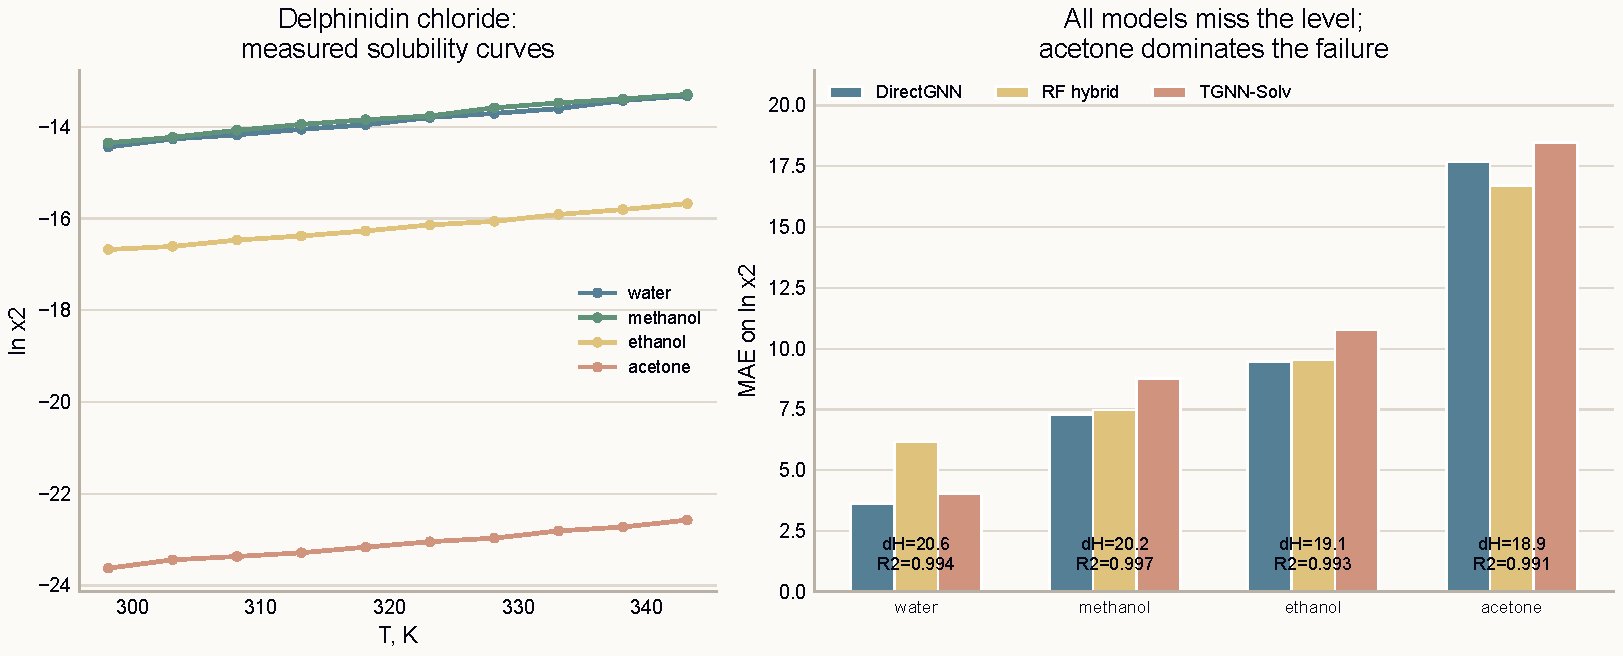
\includegraphics[width=0.96\textwidth]{delphinidin_case_study.pdf}
\caption{Дельфинидин-хлорид как локальный разбор экстремального хвоста. Слева --- экспериментальные температурные кривые, справа --- ошибки моделей по растворителям.}
\label{fig:app-delphinidin-case-study}
\end{figure}

\subsection{Внешние модели и проверка моделируемости корпуса}

Внешние ориентиры показывают, что DirectGNN находится на уровне сильных практических моделей, а не выигрывает только у слабых внутренних проверок. SolProp в режиме дообучения на целевых величинах TGNN-Solv на разбиении по новым веществам даёт $\mae=1.624$ и $\Rtwo=0.388$. Здесь это дообученная модель в том же контракте данных; по смыслу она ближе к сравнению архитектур, чем к независимой валидации опубликованных весов. FastSolv после исправления преобразования $\ln x_2\to\log S$ запускается корректно, но остаётся слабее: $\mae=1.941$, $\Rtwo=0.226$. Исправление касалось не самой физики FastSolv, а адаптера: нечисловые цели возникали из-за отсутствующих оценок молярности растворителя и строк воды с точным $\ln x_2=0$. Такие цели должны фильтроваться до масштабирования.

Чтобы оценить, не слишком ли корпус шумный для обучения, был выполнен ориентир ближайшего соседа по химическому сходству. Простейший ближайший сосед даёт $\mae=2.530$ и $\Rtwo=-0.192$, то есть существенно хуже обучаемых моделей. Следовательно, модели действительно извлекают переносимые закономерности, а не просто копируют ближайший пример.

\begin{figure}[!htbp]
\centering
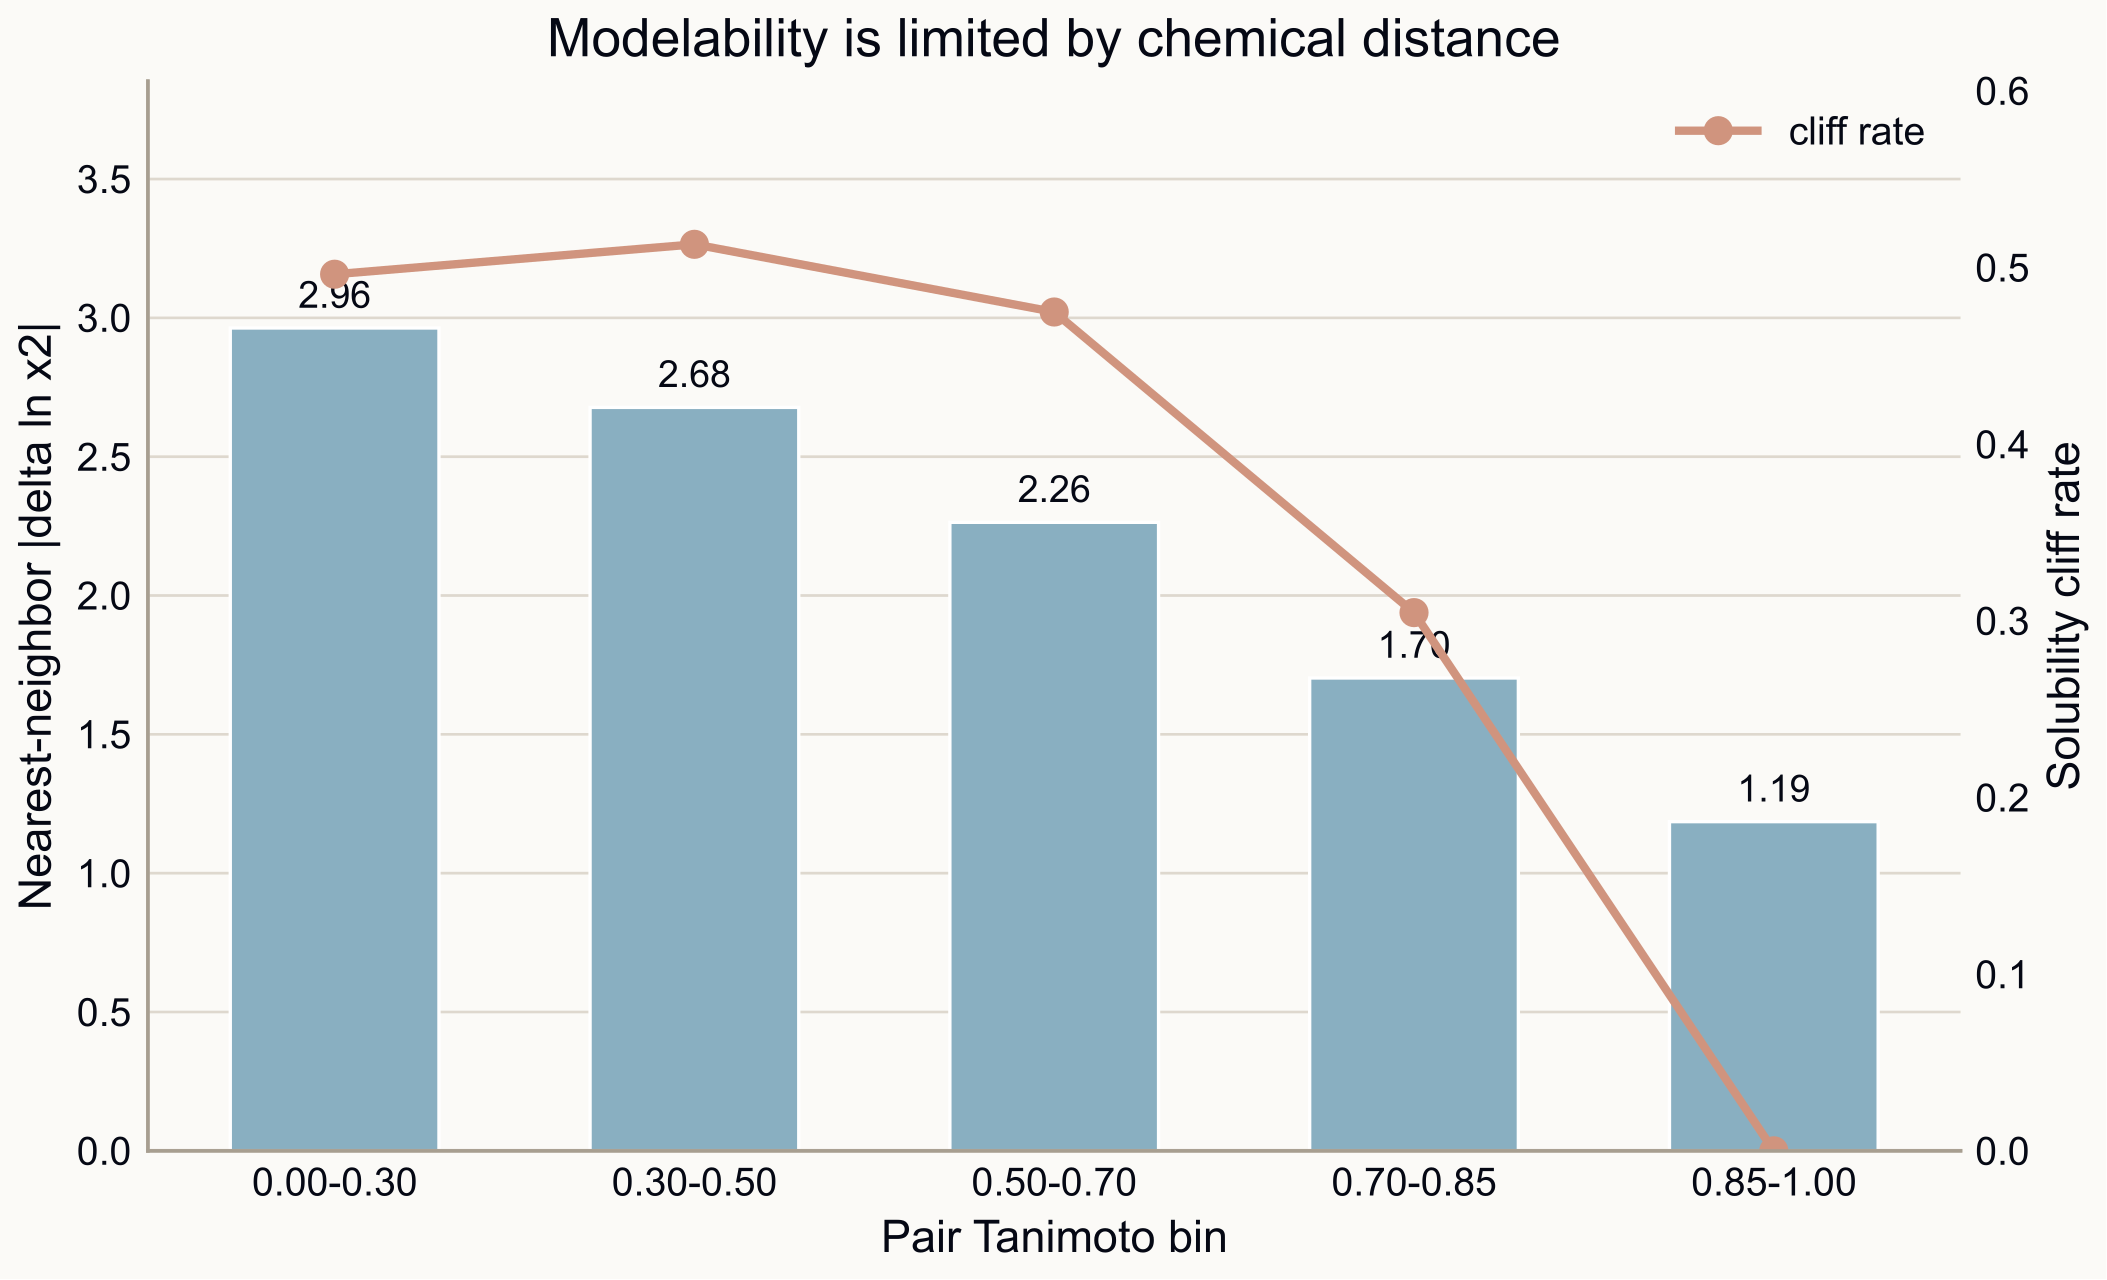
\includegraphics[width=0.90\textwidth]{knn_modelability_diagnostics_raster.png}
\caption{Проверка моделируемости через ближайшего соседа. Ошибка ближайшего обучающего примера остаётся высокой; задача не сводится к поиску похожей строки.}
\label{fig:app-knn-modelability}
\end{figure}

\subsection{Температурные эксперименты и уровень кривых}

Температурная часть является самой сильной физической диагностикой проекта. Аудит протокола показал, что низкотемпературная обучающая и высокотемпературная тестовая части имеют $100\%$ пересечение пар. Аппроксимация Вант-Гоффа с ошибкой $0.368$ --- это ориентир в режиме известной пары, а не модель для новых систем.

\begin{figure}[!htbp]
\centering
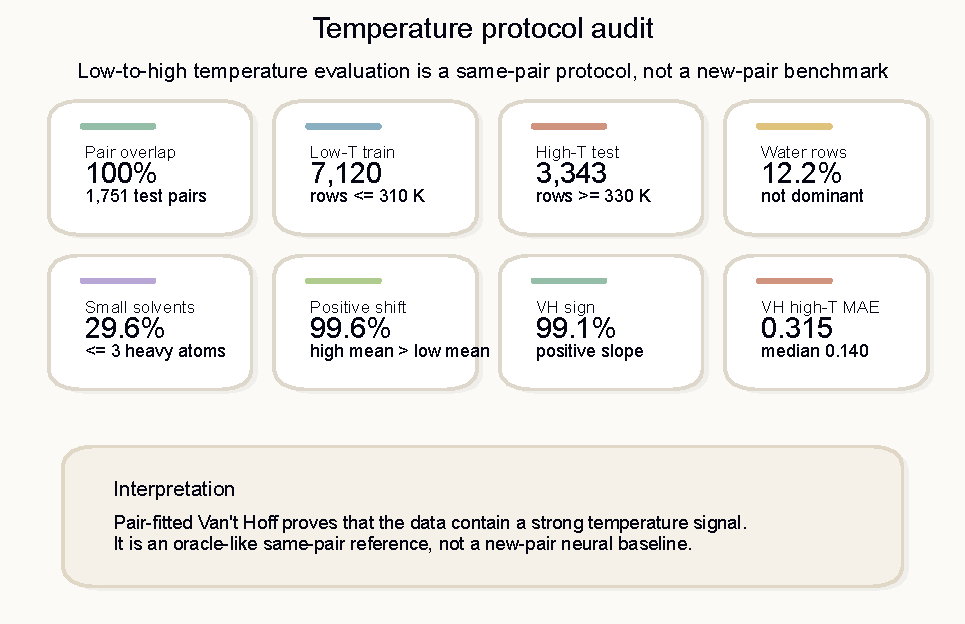
\includegraphics[width=0.82\textwidth]{temperature_protocol_audit.pdf}
\vspace{0.5em}
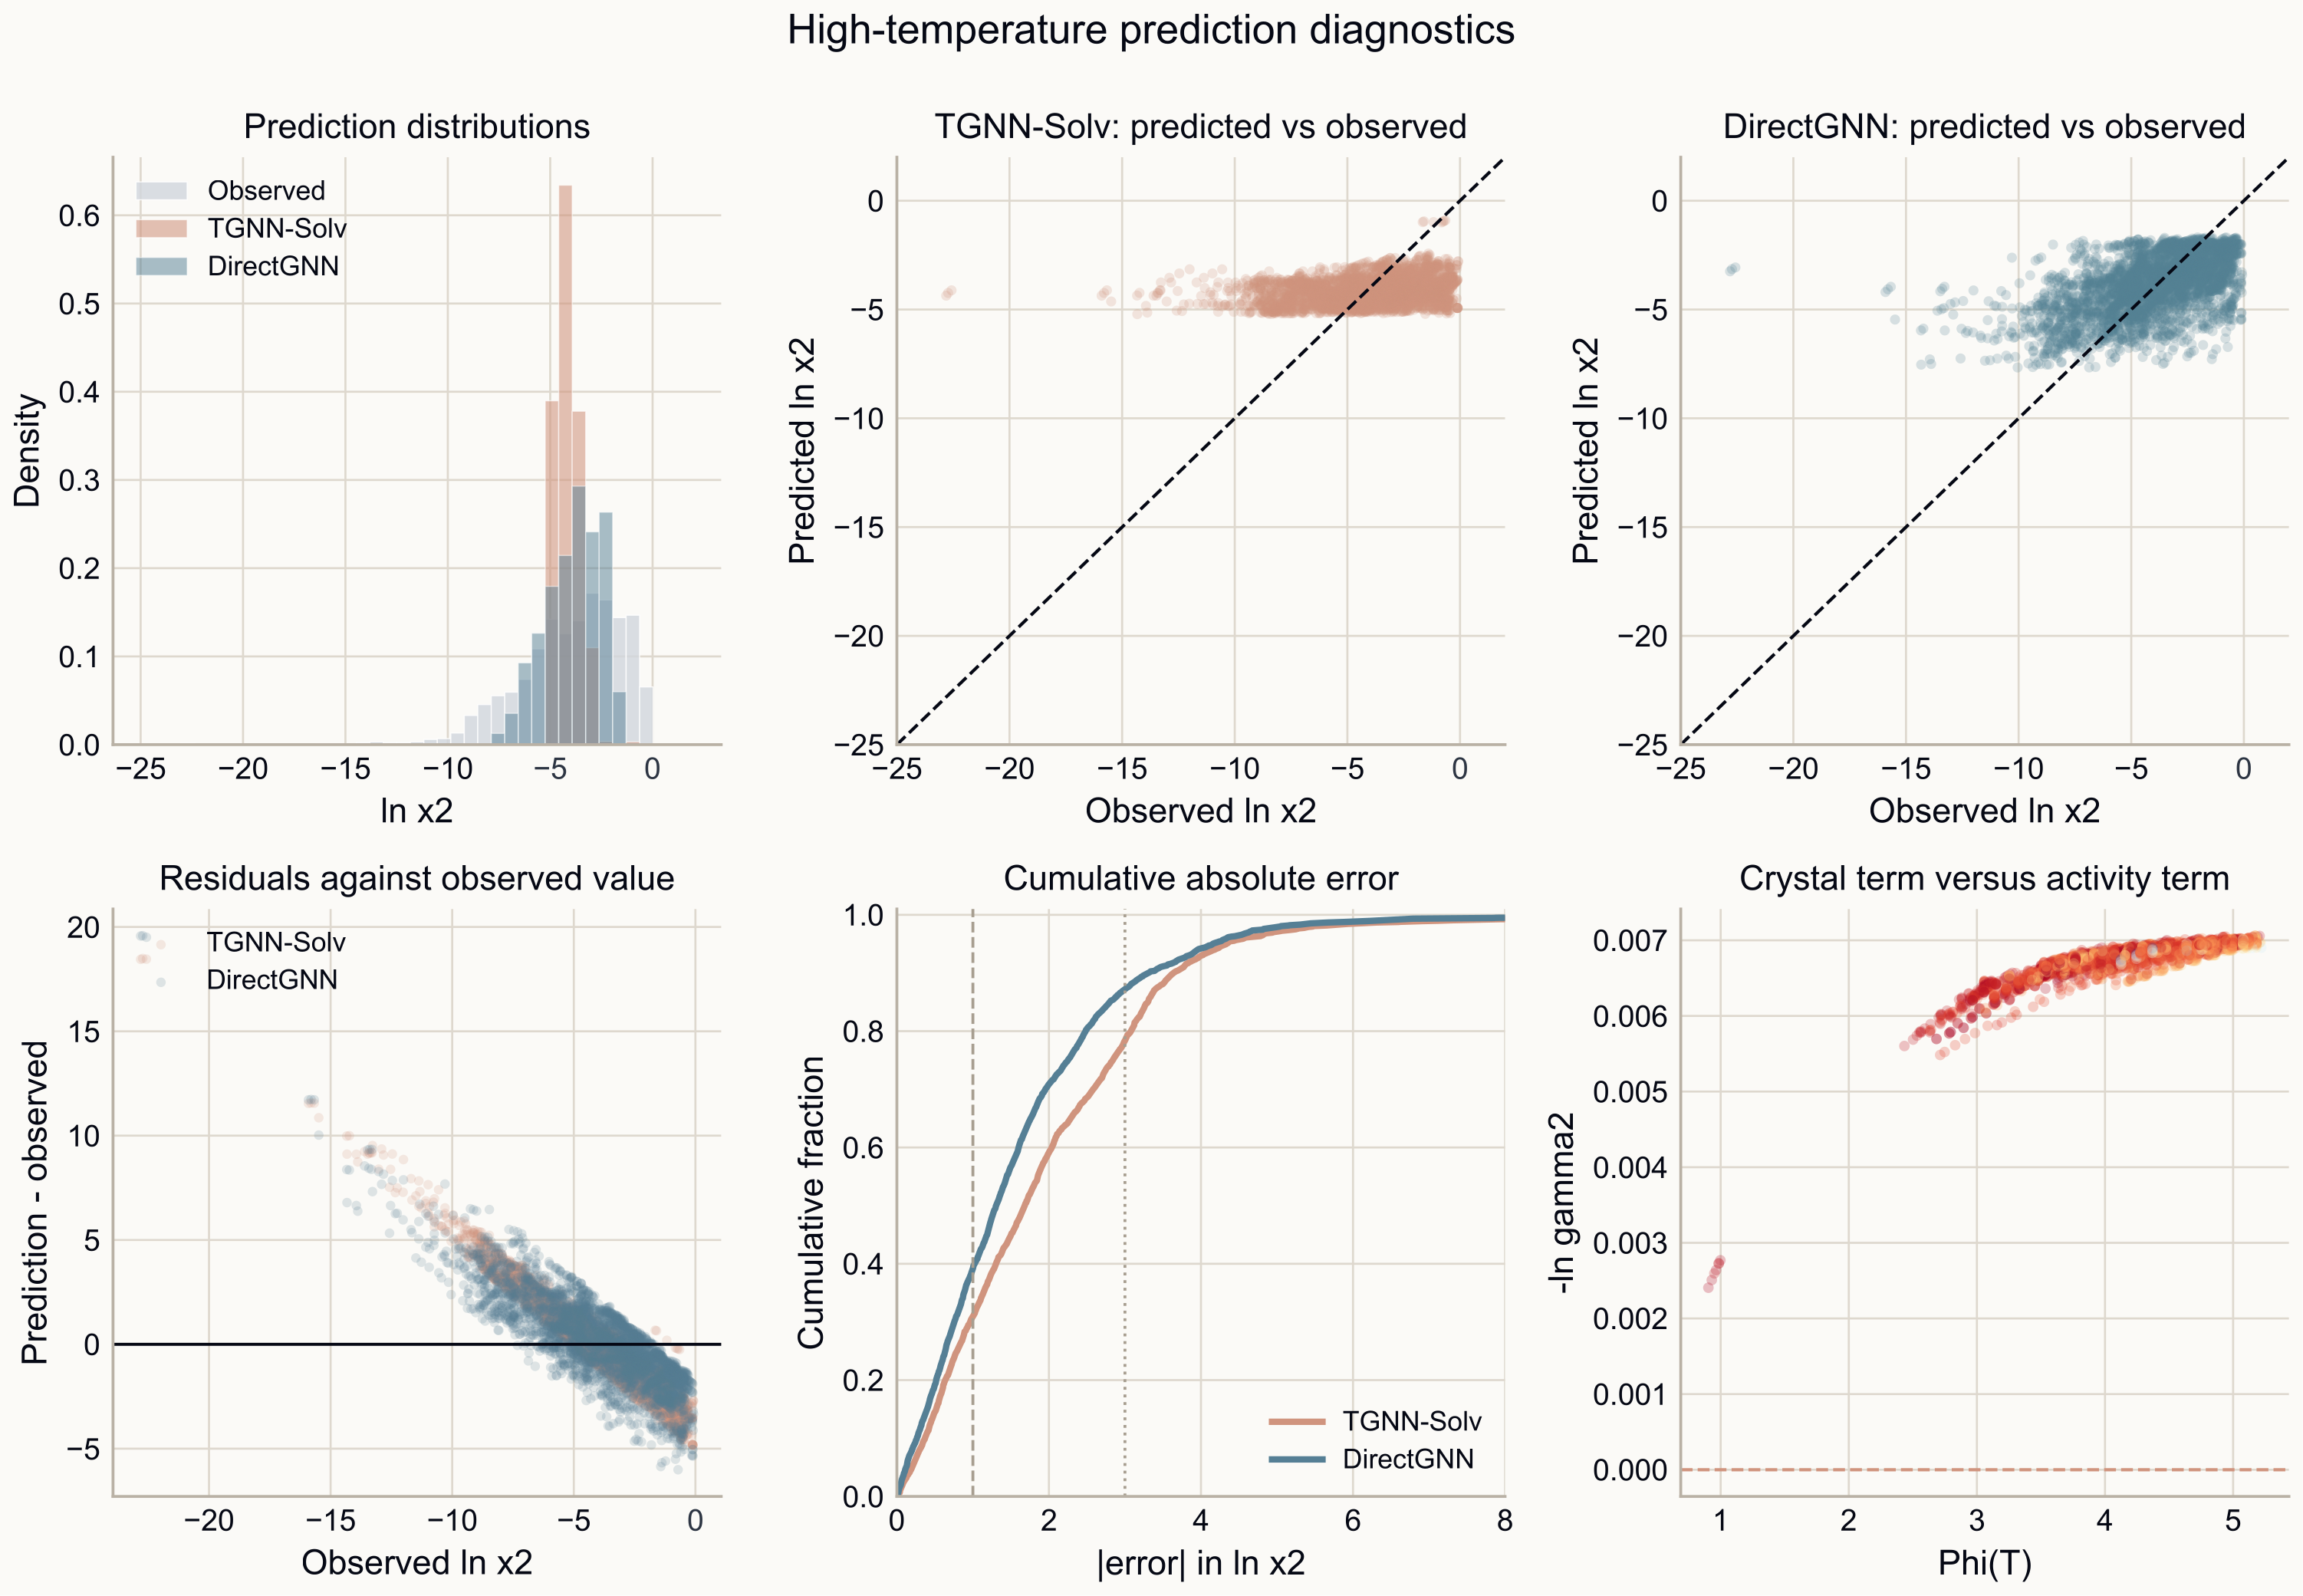
\includegraphics[width=0.82\textwidth]{temperature_prediction_distribution_diagnostics_raster.png}
\caption{Аудит температурного протокола и распределения температурных предсказаний. Верхняя панель показывает, что тест Вант-Гоффа относится к режиму известной пары; нижняя показывает сжатие диапазона предсказаний и проблему уровня кривой.}
\label{fig:app-temperature-protocol-audit}
\label{fig:app-temperature-distribution}
\end{figure}

\begin{figure}[!htbp]
\centering
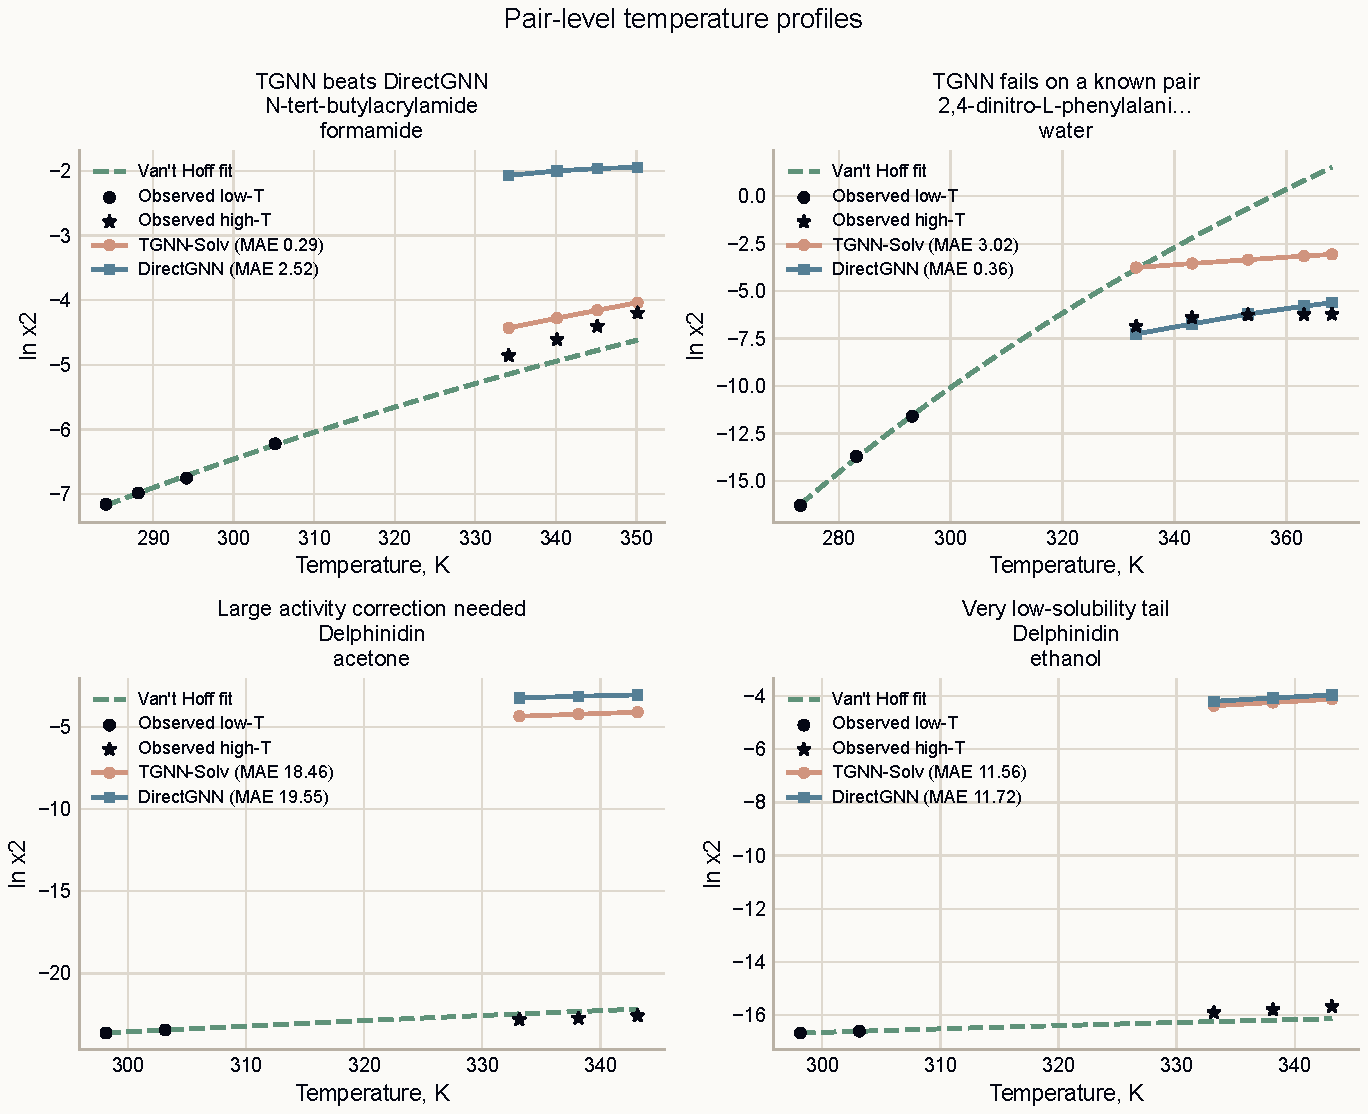
\includegraphics[width=0.94\textwidth]{temperature_pair_profile_panels.pdf}
\caption{Профили температурных пар. Такие панели нужны, чтобы видеть не только среднюю ошибку, но и форму кривых по отдельным системам.}
\label{fig:app-temperature-pair-profiles}
\end{figure}

\begin{figure}[!htbp]
\centering
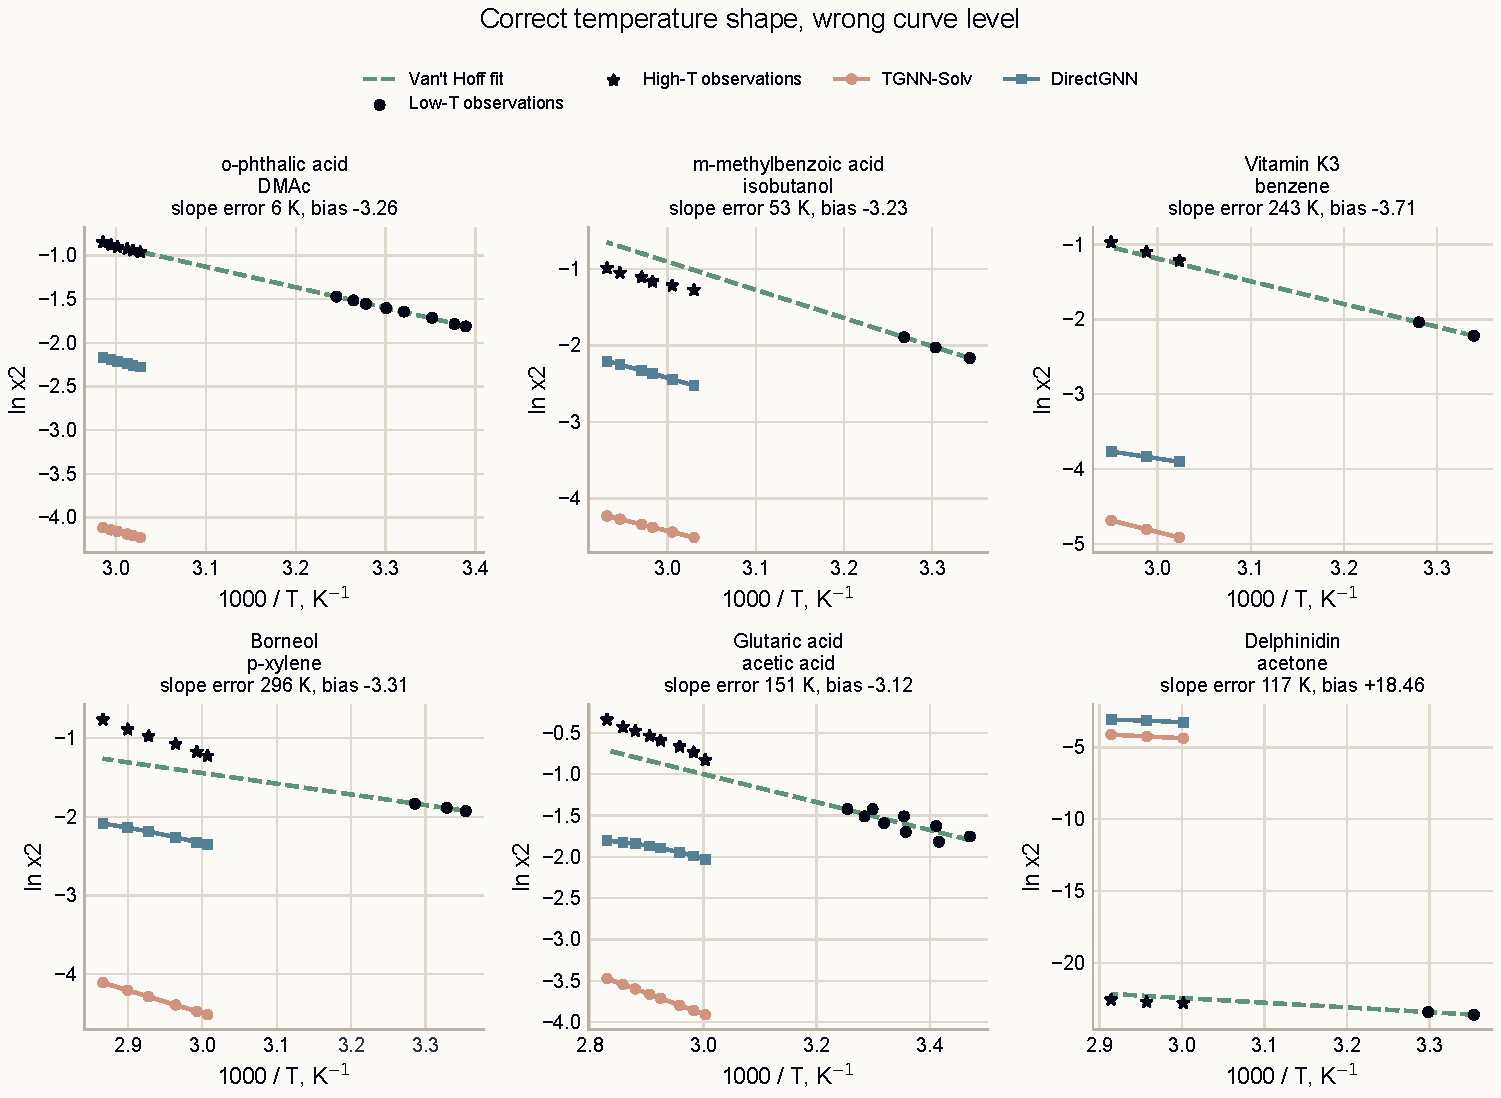
\includegraphics[width=0.92\textwidth]{temperature_slope_level_problem.pdf}
\caption{Проблема «правильный наклон, неправильный уровень». TGNN-Solv может уловить температурную форму, но завысить или занизить всю кривую из-за слабого вклада активности.}
\label{fig:app-temperature-slope-level}
\end{figure}

\begin{figure}[!htbp]
\centering
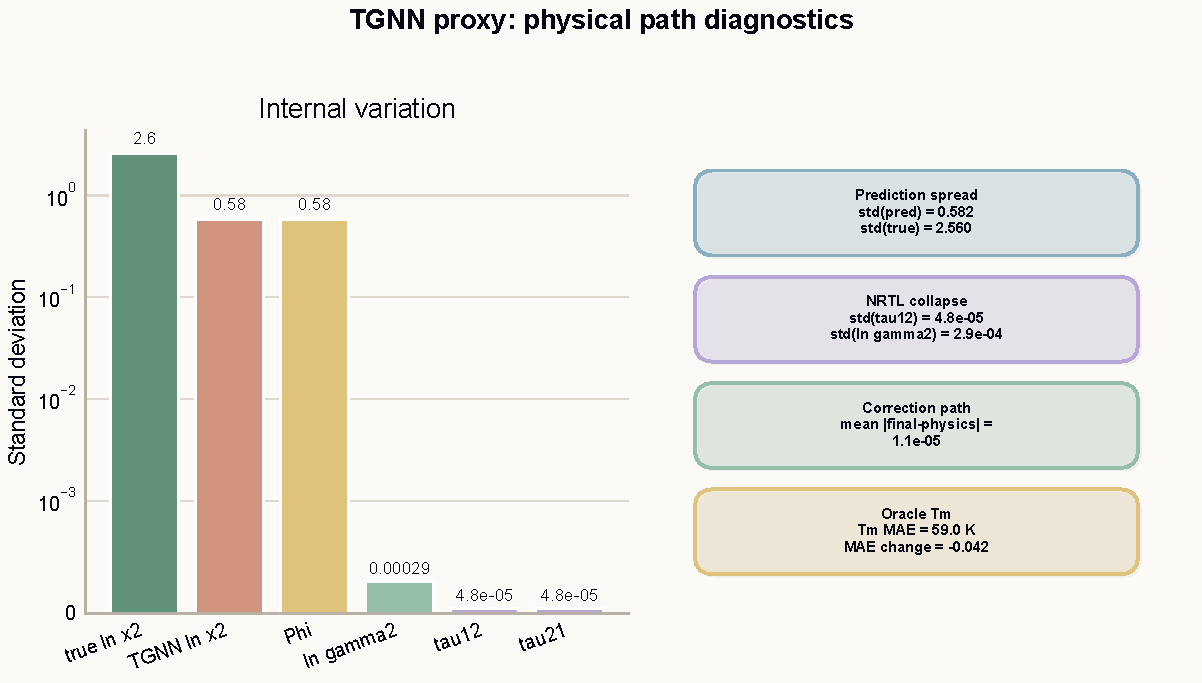
\includegraphics[width=0.92\textwidth]{temperature_tgnn_internal_diagnostics.pdf}
\caption{Внутренние величины TGNN-Solv на температурной проверке. Диагностика показывает малый разброс NRTL-параметров и сжатый диапазон итоговых предсказаний.}
\label{fig:app-temperature-internals}
\end{figure}

\begin{figure}[!htbp]
\centering
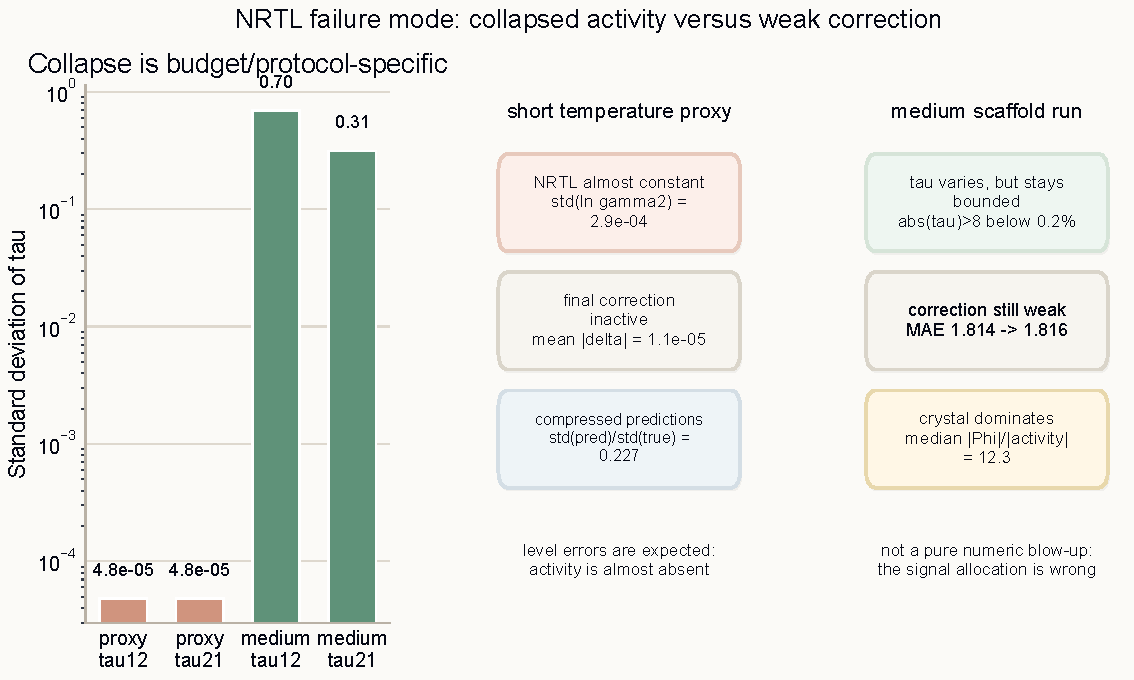
\includegraphics[width=0.90\textwidth]{nrtl_collapse_mechanism.pdf}
\caption{Вырождение NRTL-ветви. Если $\tau_{12}$ и $\tau_{21}$ почти не различаются между парами, TGNN-Solv фактически приближается к модели идеальной растворимости с небольшими поправками.}
\label{fig:app-nrtl-collapse}
\end{figure}

Главный вывод температурного блока: данные содержат сильную термодинамическую форму, но обучаемая TGNN-Solv в диагностическом запуске не восстанавливает парно-специфичный уровень активности. Полноразмерная проверка должна измерять не только MAE, но и разброс $\tau$, вклад $\ln\gamma_2$, наклон Вант-Гоффа, уровень кривой и нормы градиентов по NRTL-головам. Без такой диагностики нельзя отличить слабый обучающий сигнал от технического затухания градиента через решатель.

\subsection{Структурная экстраполяция и химические срезы}

Структурная экстраполяция остаётся трудной для всех моделей. Ошибки распределены неоднородно по химическим классам: TGNN-Solv может выигрывать в одних областях и проигрывать в других. Общий MAE не должен быть единственным критерием.

\begin{figure}[!htbp]
\centering
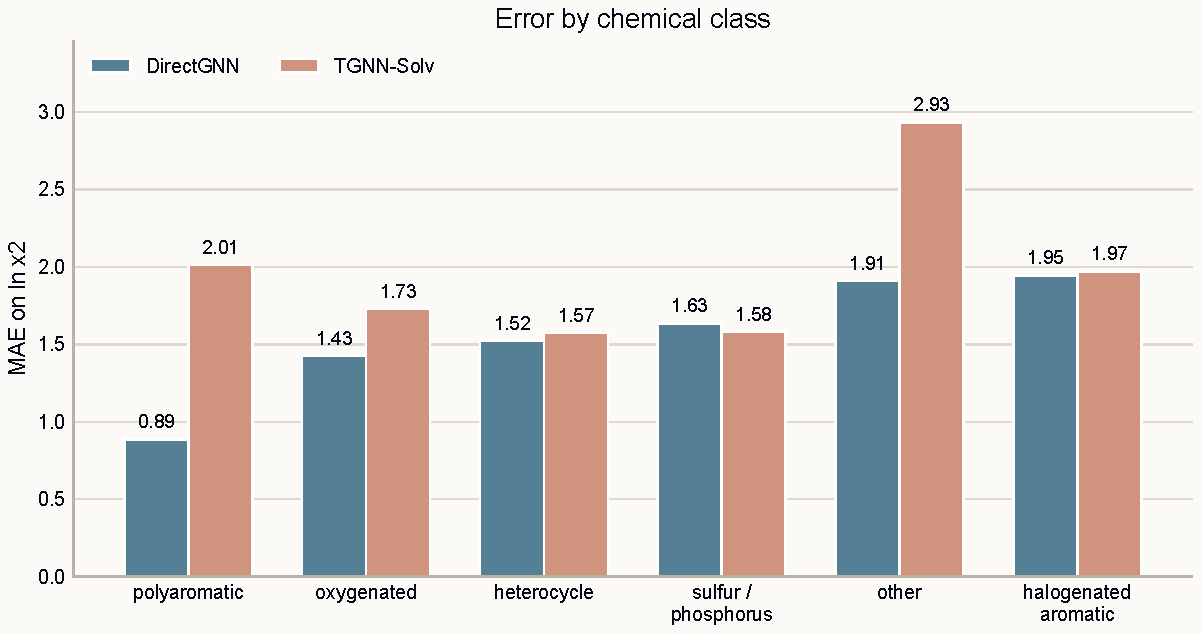
\includegraphics[width=0.88\textwidth]{prediction_slice_chemistry_class_mae.pdf}
\caption{Ошибки по химическим классам. Физический путь помогает и вредит в разных областях химического пространства.}
\label{fig:app-chemistry-class-mae}
\end{figure}

BRICS-анализ показывает, что тест по новым каркасам не сводится к простой рекомбинации уже известных фрагментов. Только $25.5\%$ тестовых растворяемых веществ полностью покрыты обучающими фрагментами, $29.5\%$ покрыты частично, а $45.0\%$ имеют преимущественно новые фрагменты. Ошибка растёт при переходе к новым фрагментам, особенно для TGNN-Solv.

\begin{figure}[!htbp]
\centering
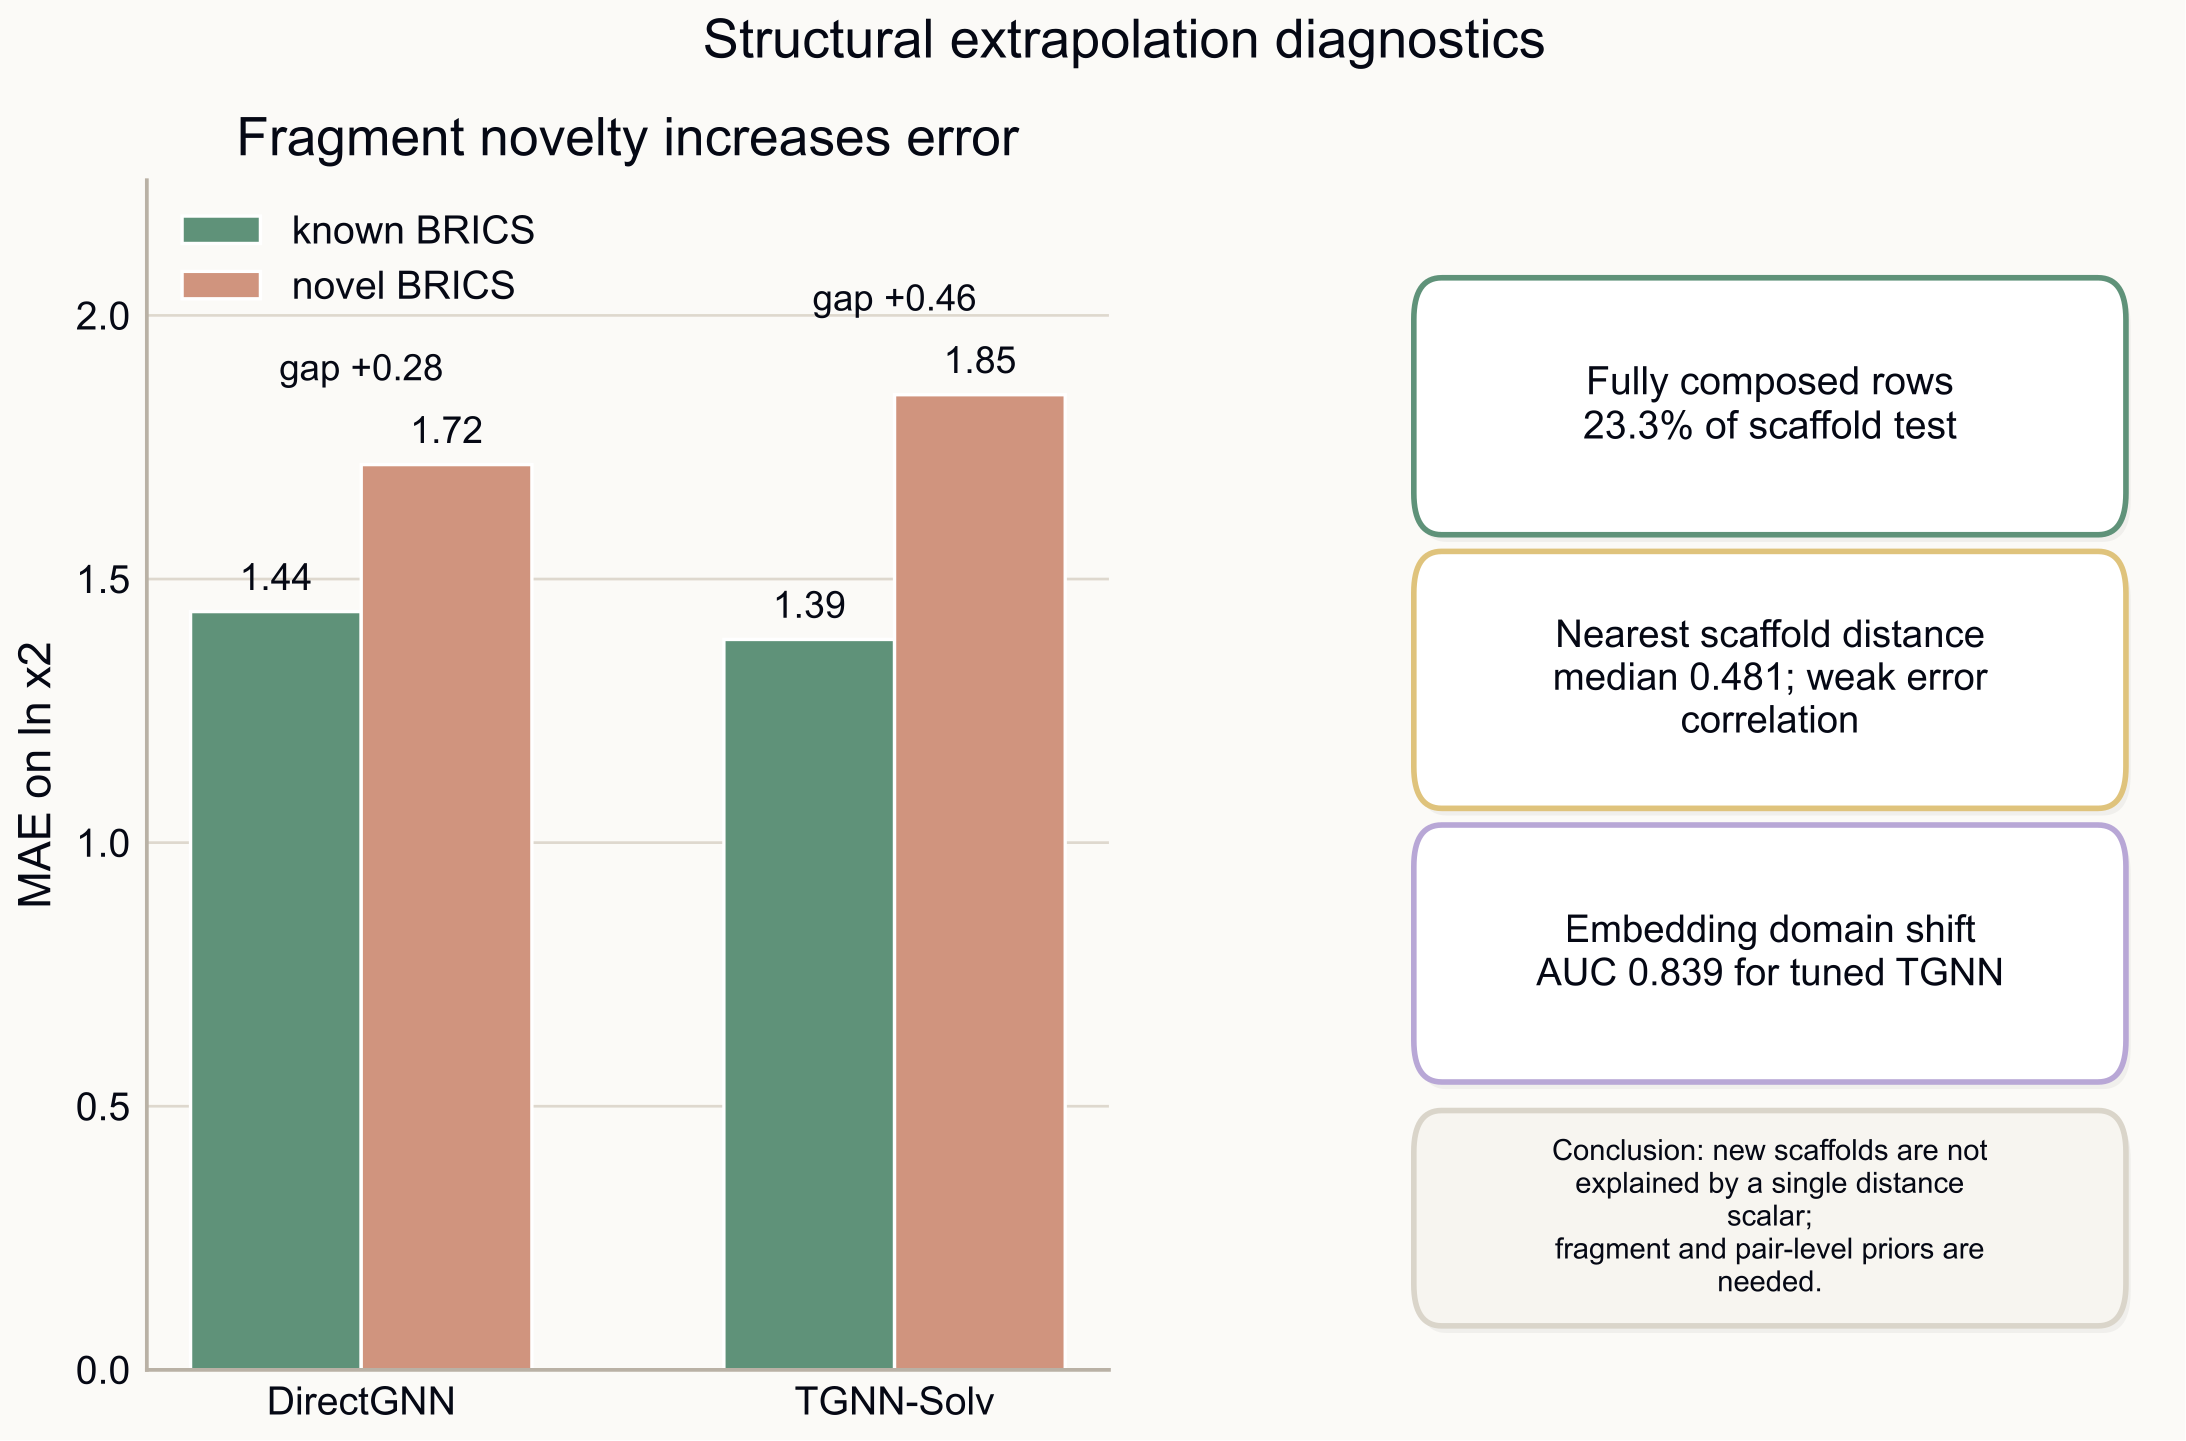
\includegraphics[width=0.92\textwidth]{structural_generalization_diagnostics_raster.png}
\caption{Диагностика структурной экстраполяции. Новизна фрагментов связана с ростом ошибки, но одно ближайшее расстояние до обучающего каркаса объясняет ошибку слабо.}
\label{fig:app-structural-generalization}
\end{figure}

\begin{figure}[!htbp]
\centering
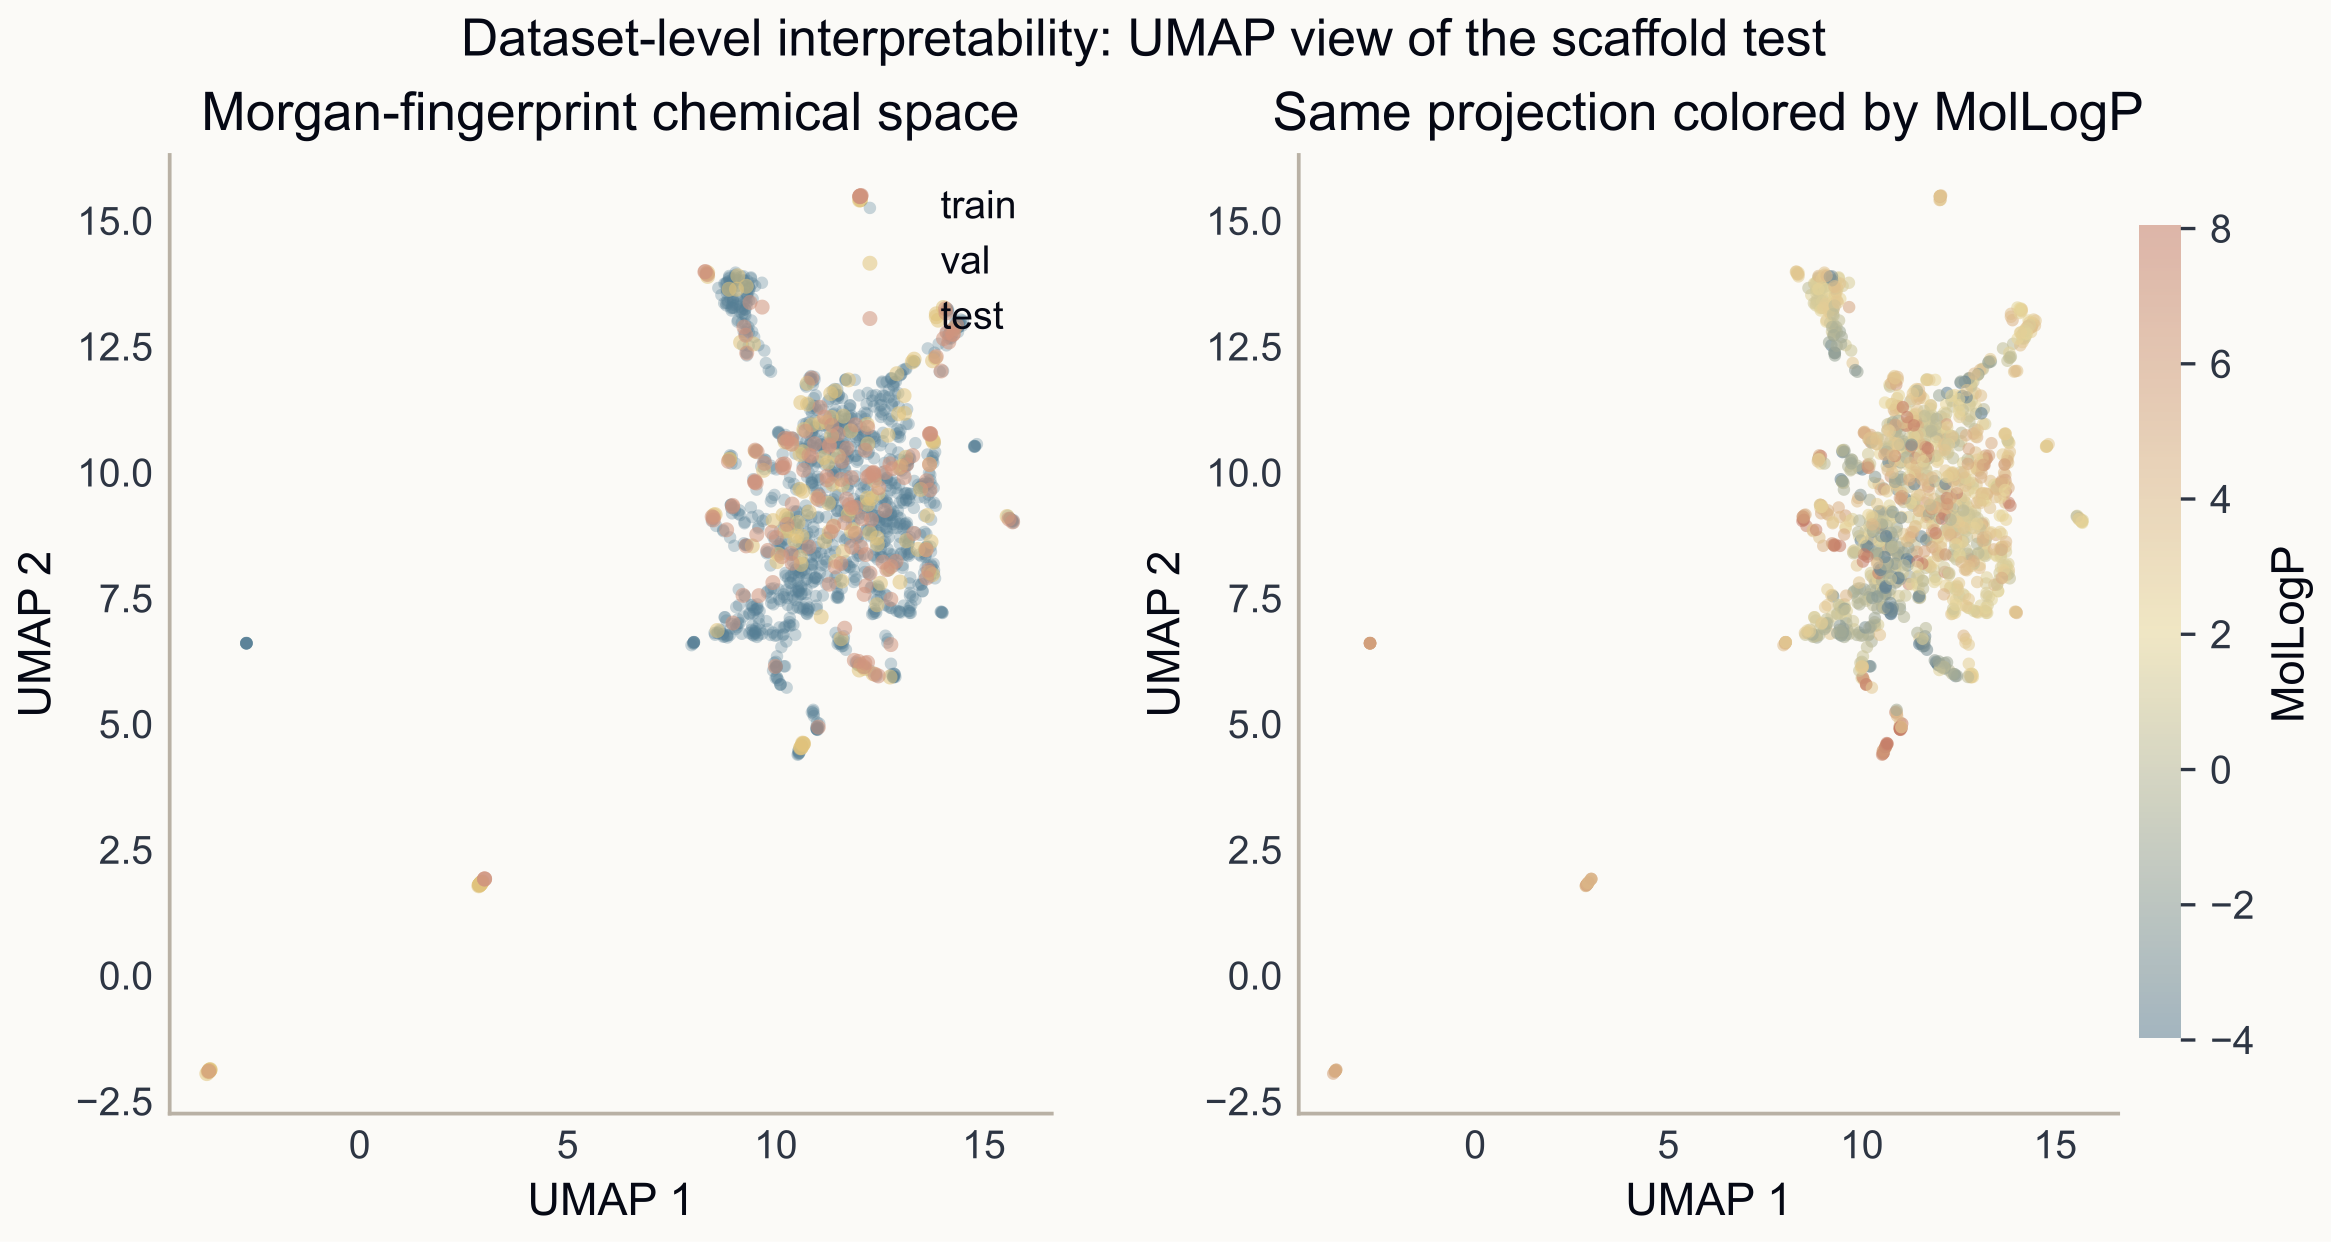
\includegraphics[width=0.88\textwidth]{chemical_space_projection_raster.png}
\caption{Проекция химического пространства растворяемых веществ по отпечаткам Morgan. Тестовые вещества не являются отдельным островом, но занимают смещённые области.}
\label{fig:app-chemical-space}
\end{figure}

\begin{figure}[!htbp]
\centering
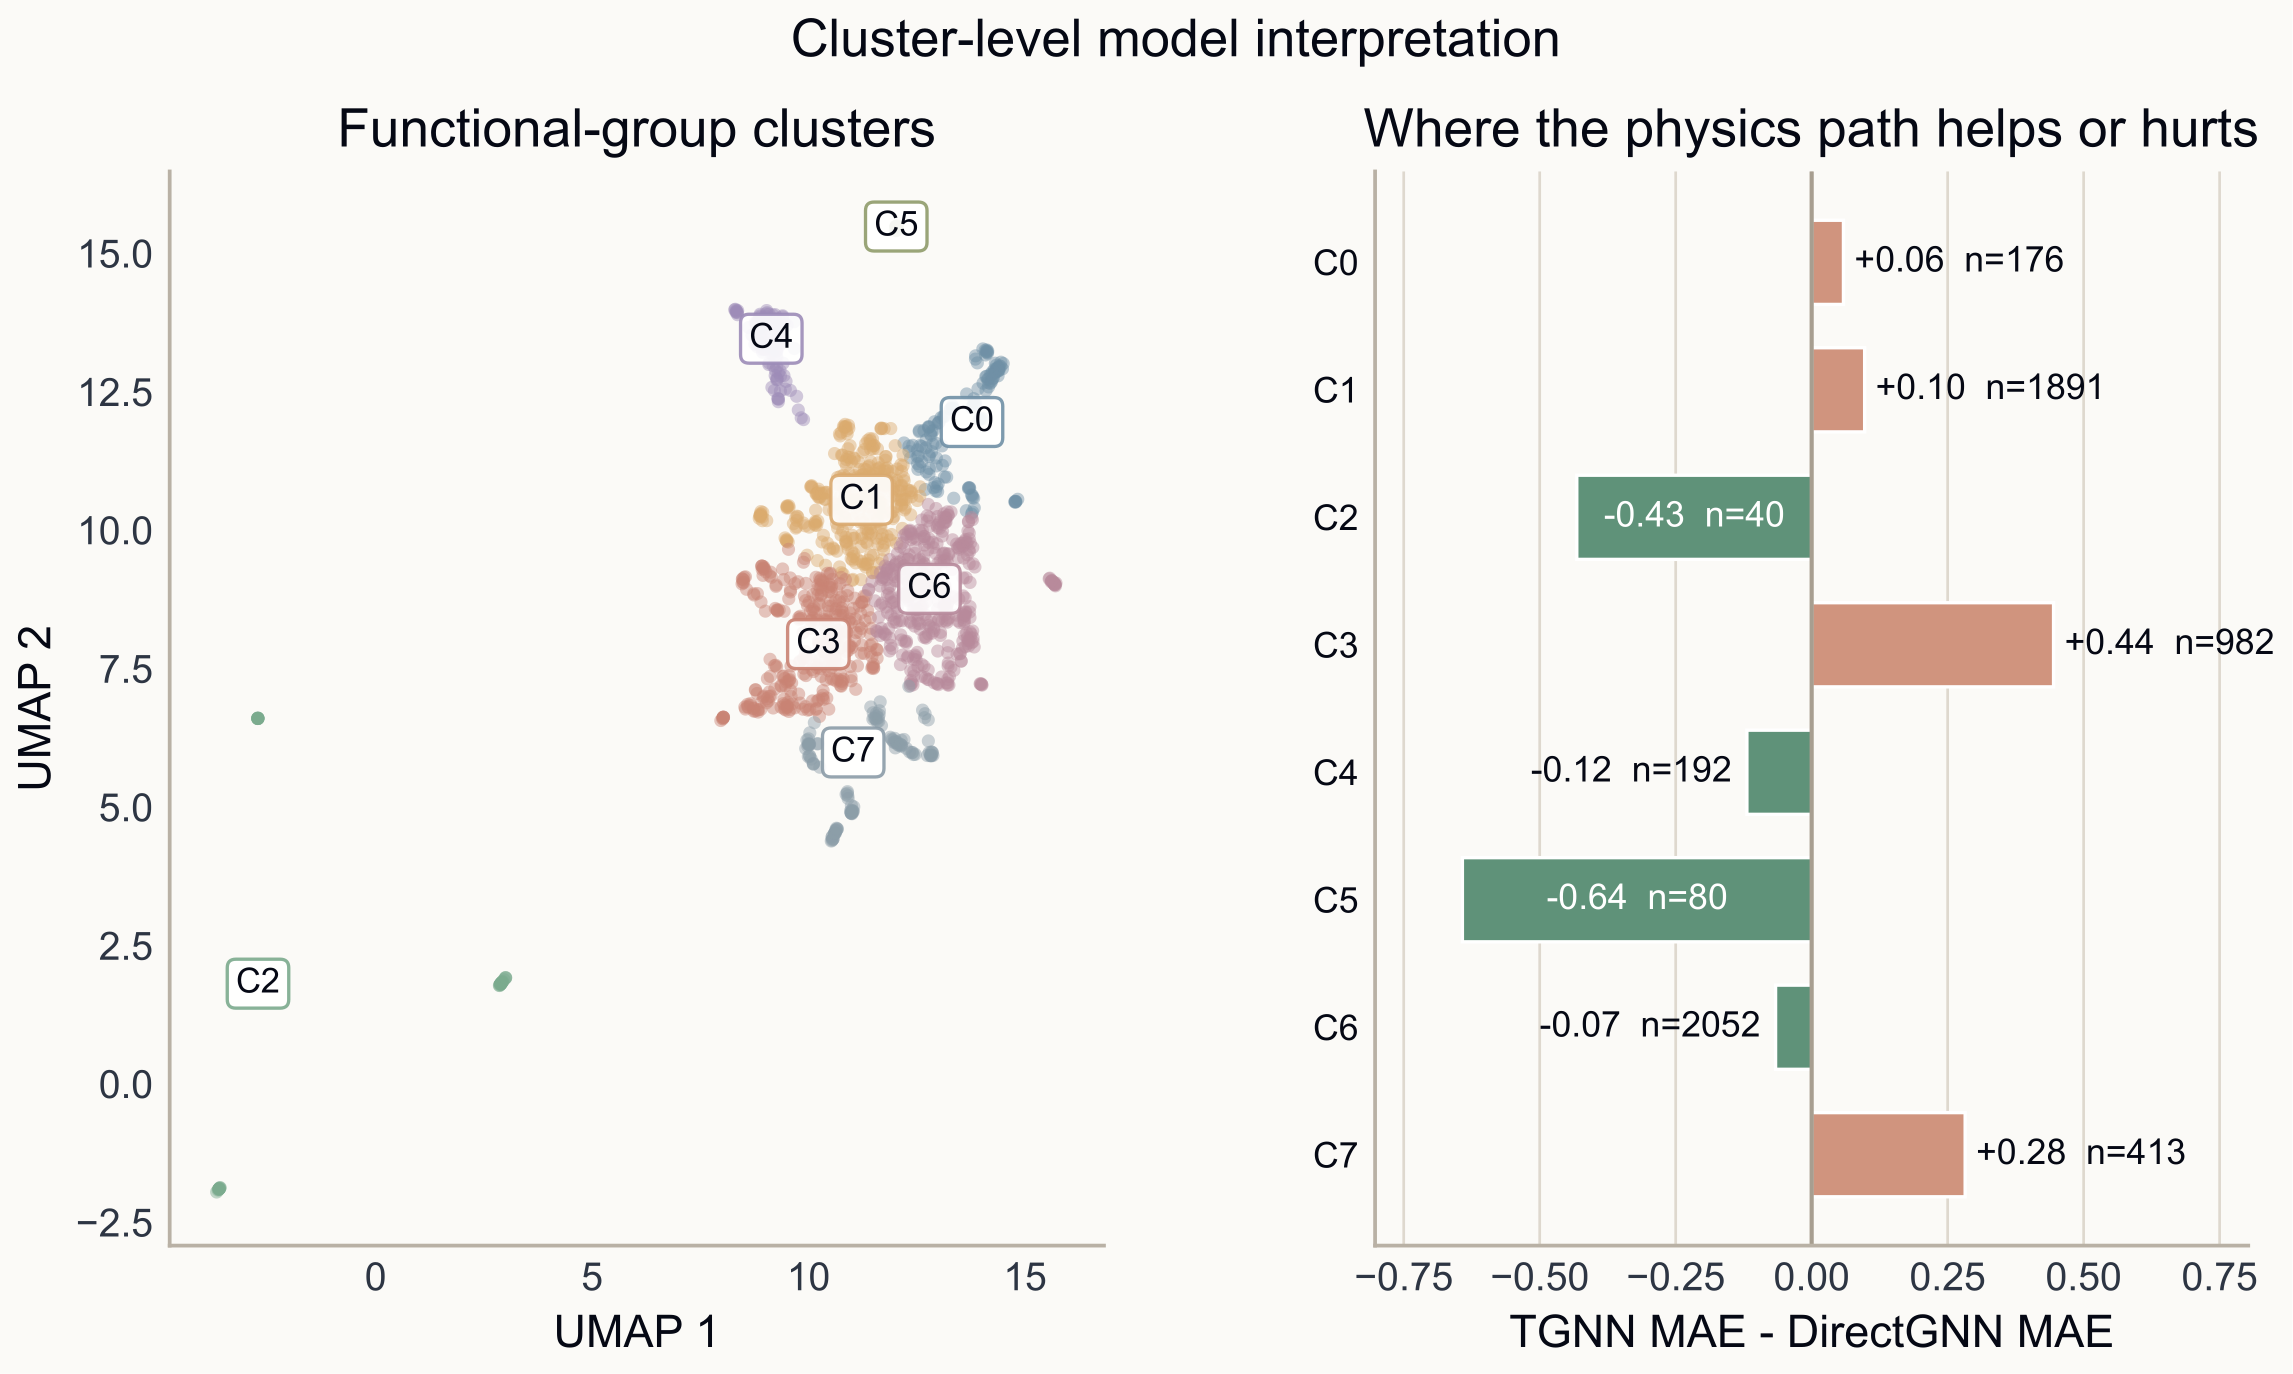
\includegraphics[width=0.90\textwidth]{cluster_error_interpretability_raster.png}
\caption{Кластерная интерпретация химического пространства. Разные группы показывают разные знаки разницы ошибок TGNN-Solv и DirectGNN.}
\label{fig:app-cluster-errors}
\end{figure}

Кластеры на UMAP следует читать как диагностические группы, а не как «истинные» химические семейства. Они получены по отпечаткам Morgan и затем интерпретированы через функциональные группы и дескрипторы RDKit. Такой срез показывает, какие химические области дают выигрыш физическому пути, а какие остаются проблемными. Репрезентативные структуры использовались только для химической интерпретации кластеров; в тексте оставлены сами классы и выводы, а не служебные пути к таблицам.

\begin{table}[!htbp]
\centering
\caption{Химическая интерпретация UMAP-кластеров растворяемых веществ. \(\Delta\mae=\mae_{\mathrm{TGNN}}-\mae_{\mathrm{Direct}}\); отрицательное значение означает меньшую ошибку TGNN-Solv.}
\label{tab:umap-cluster-classes}
\footnotesize
\begin{tabularx}{\textwidth}{C{0.12\textwidth} P{0.31\textwidth} P{0.30\textwidth} Y}
\toprule
Кластер & Химический класс & Доминирующие признаки & Разница ошибок и вывод \\
\midrule
C0 (\(N=140\)) & Ароматические сульфоны и амины & ароматические 100\%, сульфоны 75\%, амины 75\%, галогены 43\% & \(\Delta\mae=+0.058\): разница мала. \\
C1 (\(N=362\)) & Азотсодержащие гетероароматы и карбонильные ароматические соединения & ароматические 93\%, N-гетероароматы 52\%, карбонилы 38\%, амины 33\% & \(\Delta\mae=+0.097\): DirectGNN немного лучше. \\
C2 (\(N=35\)) & Гидрофобные ароматические амины с длинными алкильными фрагментами & ароматические 91\%, амины 77\%, карбонилы 57\%, длинные алкилы 49\% & \(\Delta\mae=-0.432\): TGNN-Solv лучше, но кластер мал. \\
C3 (\(N=338\)) & Гидрокси-карбонильные кислоты, спирты и гибкие алифатические фрагменты & карбонилы 78\%, гидроксилы 68\%, карбоксилы 41\%, амины 32\% & \(\Delta\mae=+0.445\): главный крупный проблемный кластер TGNN-Solv. \\
C4 (\(N=126\)) & Нитроароматические амины и полярные нитросоединения & амины 99\%, нитрогруппы 95\%, ароматические 94\%, карбонилы 33\% & \(\Delta\mae=-0.119\): физический путь не хуже прямого, но разрыв невелик. \\
C5 (\(N=11\)) & Малый тестовый кластер гидрофобных длинноцепочечных ароматических аминов & длинные алкилы 100\%, ароматические 100\%, амины 100\%, галогены 45\% & \(\Delta\mae=-0.642\): TGNN-Solv лучше; \(73\%\) веществ в тестовой части. \\
C6 (\(N=398\)) & Ароматические карбонильные, фенольные и эфирные соединения & ароматические 99\%, карбонилы 74\%, гидроксилы 58\%, эфиры 46\% & \(\Delta\mae=-0.066\): широкий смешанный кластер, разница мала. \\
C7 (\(N=115\)) & Крупные гибкие гидрокси- и эфирсодержащие молекулы с длинными цепями & длинные алкилы 70\%, гидроксилы 67\%, ароматические 65\%, эфиры 49\% & \(\Delta\mae=+0.282\): TGNN-Solv хуже; вероятна нехватка описания гибкости и ассоциации. \\
\bottomrule
\end{tabularx}
\end{table}

\begin{figure}[!htbp]
\centering
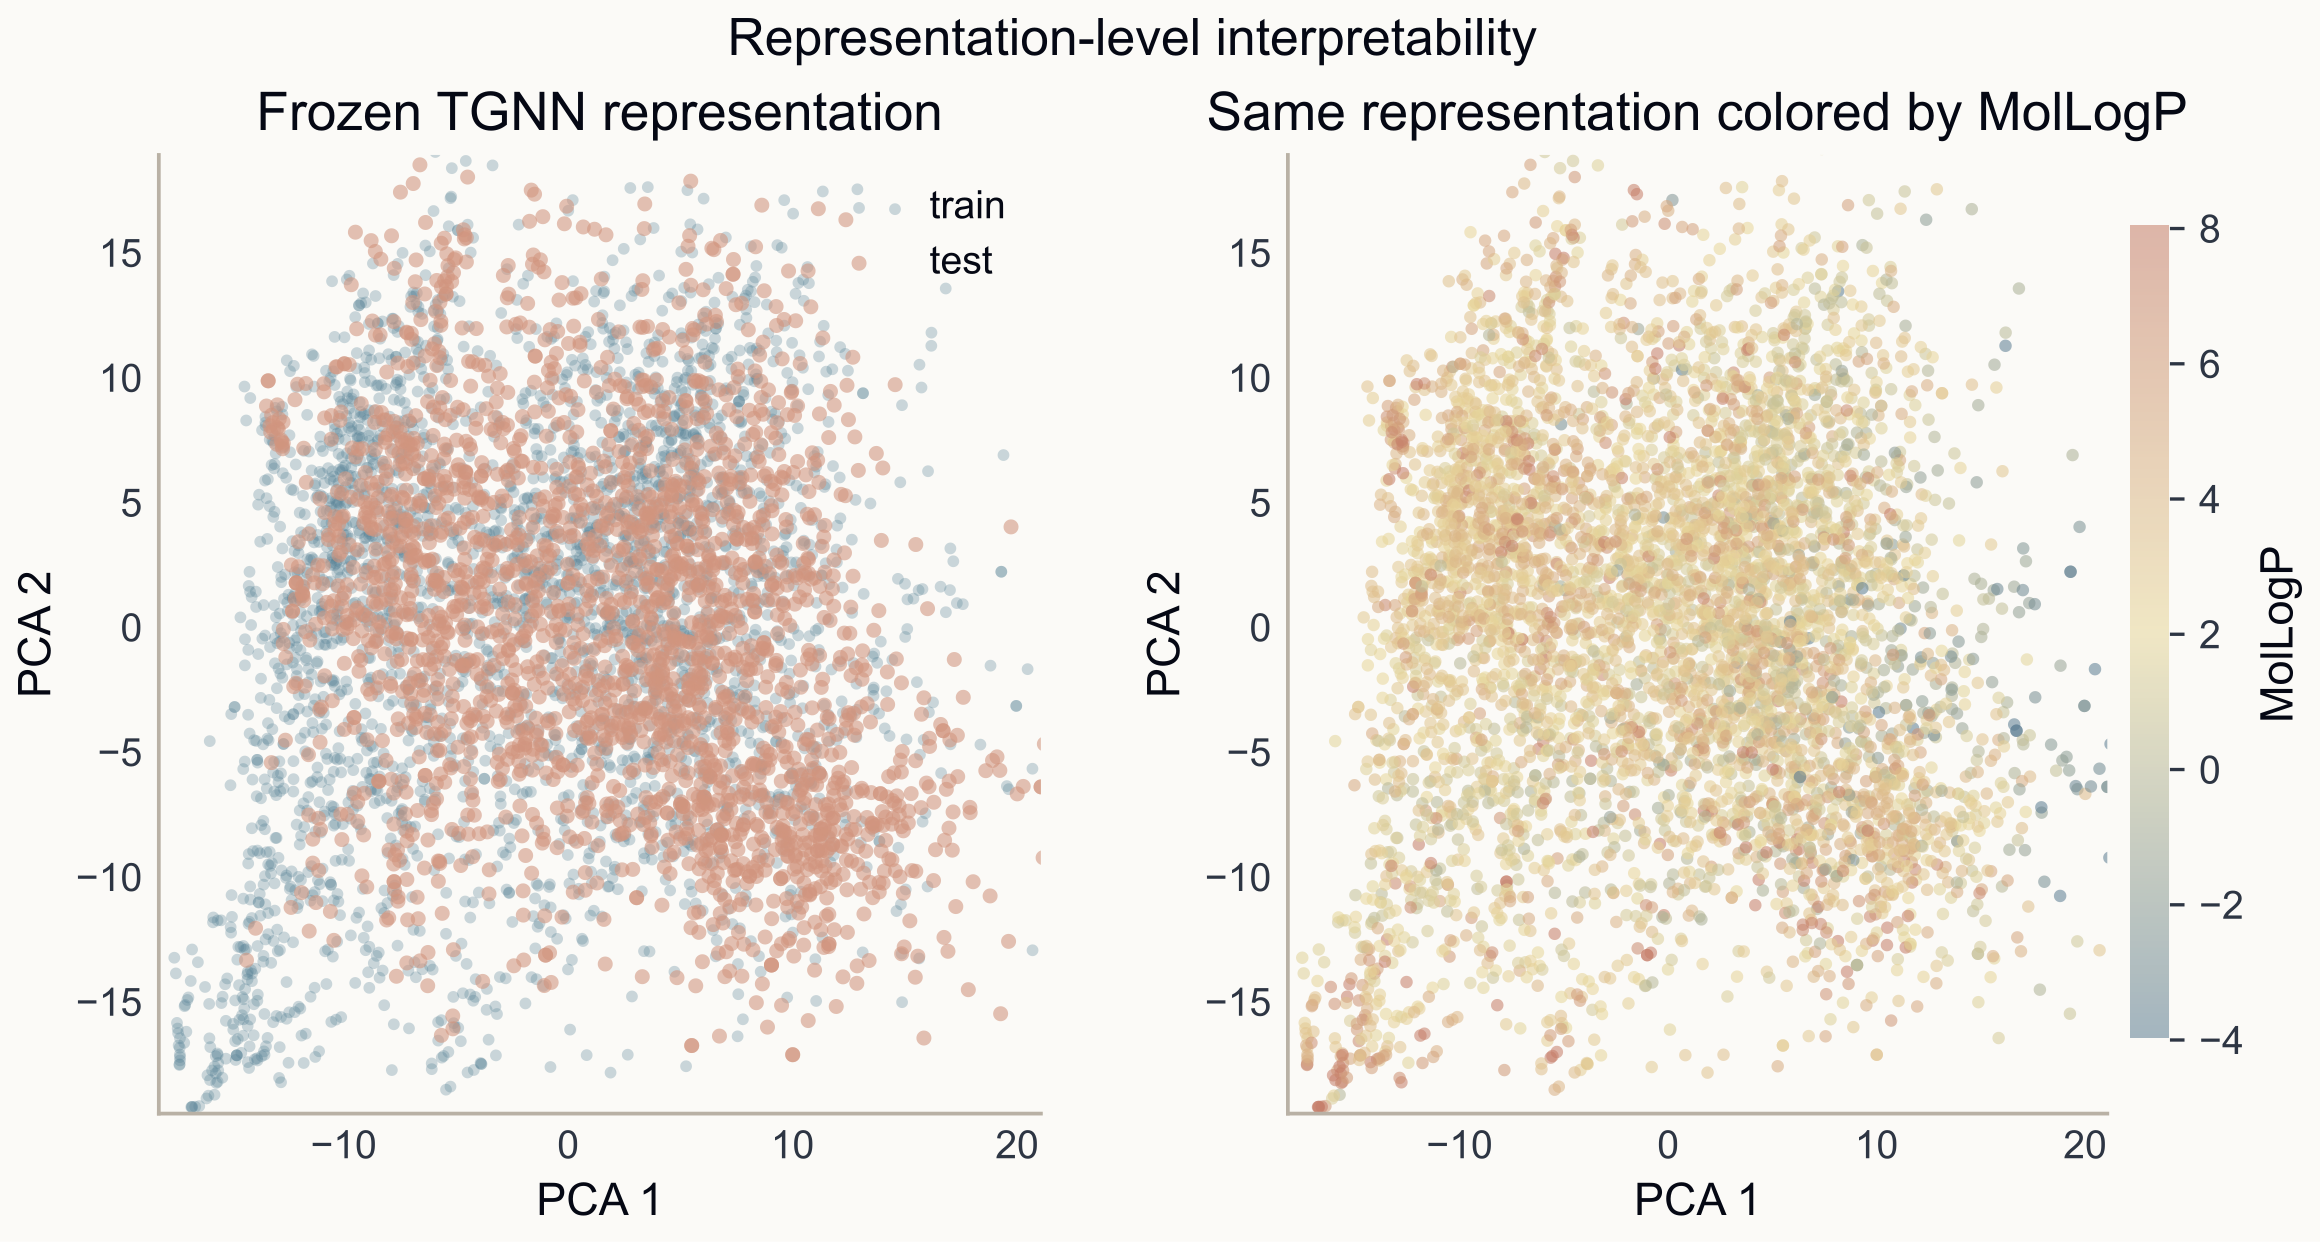
\includegraphics[width=0.88\textwidth]{embedding_geometry_diagnostics_raster.png}
\caption{Геометрия скрытых представлений TGNN-Solv. Обучающая и тестовая части не полностью перемешиваются в пространстве признаков, что поддерживает гипотезу о необходимости лучшего парного и фрагментного представления.}
\label{fig:app-embedding-geometry}
\end{figure}

\subsection{Рабочие гипотезы и отрицательные результаты}

В проекте накоплены не только положительные идеи, но и отрицательные проверки. Это важно: они не дают объяснять любую ошибку произвольной новой гипотезой.

\begin{figure}[!htbp]
\centering
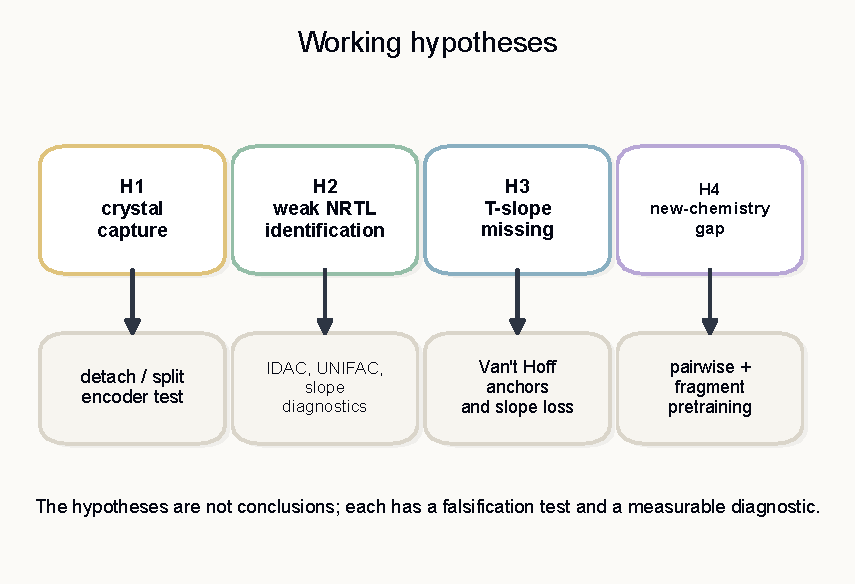
\includegraphics[width=0.94\textwidth]{hypothesis_map_schematic.pdf}
\caption{Карта рабочих гипотез. Каждая гипотеза связана с заданной проверкой: кристаллическая ветвь, идентифицируемость NRTL, температурный наклон, парное представление и систематические физические ошибки.}
\label{fig:app-hypothesis-map}
\end{figure}

Проверенные отрицательные результаты:
\begin{itemize}
    \item преобразование единиц между $\ln x_2$ и $\log S$ не объясняет наблюдаемую MAE; ошибка обратного преобразования находится около машинной точности;
    \item удаление экстремального хвоста $\ln x_2<-15$ улучшает $\Rtwo$ только примерно на $0.01$--$0.02$: хвост важен, но одной этой причиной проблему не объяснить;
    \item первый вариант взвешивания источников ухудшил DirectGNN и не улучшил TGNN-Solv;
    \item простое усиление температурных ограничений в запуске с малым бюджетом не решило температурную экстраполяцию;
    \item мостовой компонент на основе классической теории регулярных растворов нельзя включать безусловно, потому что он плохо описывает выгодные специфические взаимодействия и случаи $\gamma_2<1$.
\end{itemize}

\begin{figure}[!htbp]
\centering
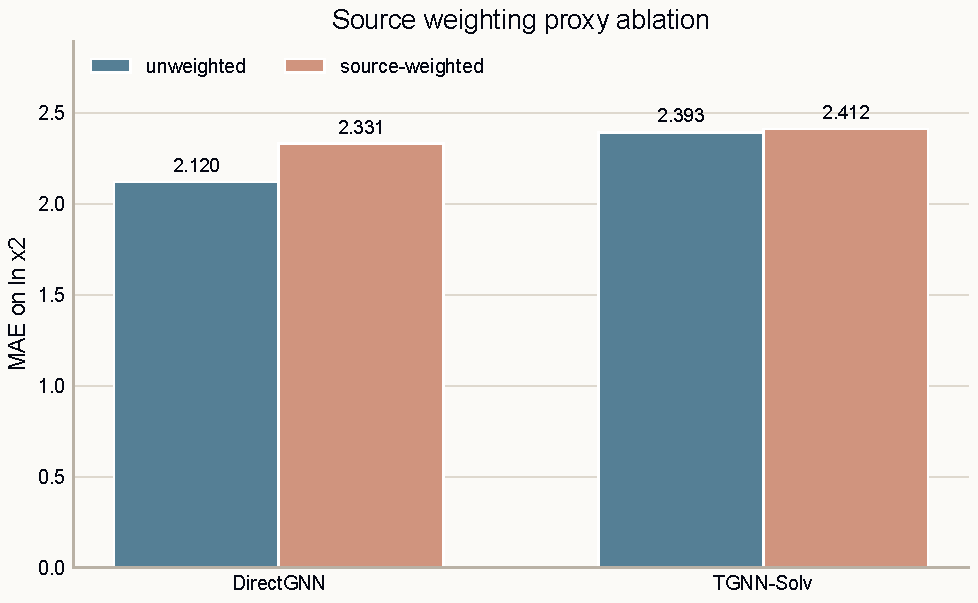
\includegraphics[width=0.82\textwidth]{source_weighting_ablation.pdf}
\caption{Проверка первого варианта весов по источникам. Взвешивание не улучшило качество и оставлено как диагностическая инфраструктура, а не как основной результат.}
\label{fig:app-source-weighting}
\end{figure}

\subsection{Предварительные проверки без полноразмерного обучения}

Отдельно были выполнены малые обучающие проверки на сбалансированном диагностическом срезе \(2\,629/704/1\,002\) строк. Их цель ограничена: проверить, дают ли новые функции ошибки и прямая температурная параметризация измеримый сигнал до дорогостоящего полноразмерного запуска. Эти числа не следует сравнивать напрямую с основной каркасной таблицей, потому что выборка и бюджет обучения другие.

\begin{table}[!htbp]
\centering
\caption{Малые диагностические прогоны новых функций ошибки и прямых физических параметризаций.}
\label{tab:small-training-diagnostics}
\small
\begin{tabularx}{\textwidth}{P{0.40\textwidth}rrrr}
\toprule
Диагностическая модель & $\mae$ & $\Rtwo$ & смещение & $\sigma(\hat y)/\sigma(y)$ \\
\midrule
DirectGNN, потеря Хьюбера & 3.134 & 0.174 & $-1.008$ & 0.745 \\
DirectGNN, взвешенная MAE & 3.053 & 0.207 & 0.011 & 0.727 \\
TGNN-Solv, прямая \(\Phi\), Вант-Гофф и взвешенная MAE & 3.416 & 0.111 & $-1.628$ & 0.733 \\
TGNN-Solv, прямой предел активности \(\ln\gamma_2^\infty(T)\) & 3.236 & 0.194 & $-1.396$ & 0.668 \\
TGNN-Solv, прямой предел активности и хвостовая потеря & 2.862 & 0.318 & $-0.430$ & 0.592 \\
\bottomrule
\end{tabularx}
\end{table}

Взвешенная MAE уменьшила среднюю ошибку DirectGNN и почти убрала глобальное смещение, но не устранила сжатие диапазона. Прямая параметризация \(\Phi(T)=a+b/T\) не улучшила среднюю ошибку TGNN-Solv в коротком прогоне, но дала лучший результат в крайнем левом хвосте \(\ln x_2<-15\): \(\mae=6.58\) против \(7.63\)--\(7.76\) у прямых диагностических моделей. Прямая параметризация предела активности дала более полезный результат: она снизила ошибку TGNN-Solv с $3.416$ до $3.236$ и подняла $\Rtwo$ с $0.111$ до $0.194$ относительно малой NRTL-версии. Направление совпадает с гипотезой о неидентифицируемости NRTL, но модель всё ещё оставалась хуже взвешенной DirectGNN ($3.053$).

Следующая проверка изменила уже не параметризацию, а функцию потерь: строки в хвостах распределения \(\ln x_2\) получили повышенный фиксированный вес. В этом малом прогоне TGNN-Solv снизила MAE до $2.862$ и стала лучше DirectGNN на том же диагностическом срезе. Среднее смещение уменьшилось почти на единицу ($-1.431\to-0.430$), а \(\Rtwo\) вырос до $0.318$. Однако отношение стандартных отклонений упало до $0.592$. Значит, хвостовая потеря помогла уровню и ранжированию, но не расширила диапазон предсказаний. Это важное ограничение: улучшение качества есть, но механизм сжатия ещё не устранён.

Близкие значения $\Rtwo$ у взвешенной DirectGNN ($0.207$) и версии с прямым пределом активности ($0.194$) не означают одинаковую калибровку. У DirectGNN смещение почти нулевое ($0.011$), а у TGNN-Solv с прямым пределом активности оно остаётся большим и отрицательным ($-1.396$). При этом ранговые корреляции у физической версии выше. Значит, замена активности улучшает форму и ранжирование относительно полной NRTL-версии, но уровень предсказаний остаётся сдвинутым вниз. Хвостовая потеря частично исправляет этот уровень, однако базовая причина всё равно требует разложения на кристаллический вклад, средний уровень \(\ln\gamma_2^\infty\) и их компенсацию.

На повторяющихся температурных парах ошибка наклона осталась большой: около \(1\,471\,\mathrm K\) для TGNN-Solv и \(1\,947\,\mathrm K\) для взвешенной DirectGNN при истинном разбросе наклонов около \(2\,070\,\mathrm K\). Версия с прямым пределом активности дала почти ту же среднюю ошибку наклона, но немного увеличила разброс предсказанных наклонов и корреляцию с истинными наклонами. Хвостовая версия сохранила преимущество над DirectGNN по наклону (\(1\,491\,\mathrm K\) против \(1\,947\,\mathrm K\)), но её предсказанные наклоны стали ещё более сжатыми. Это согласуется с общей картиной: физическая форма помогает температурной зависимости, а абсолютный уровень и амплитуда остаются слабым местом.

\subsection{Проверенные и непроверенные компоненты}

Многие компоненты уже реализованы, но не все доказали пользу в полном режиме. Чтобы не смешивать инфраструктуру и результат, степень подтверждения фиксируется явно.

\begin{table}[!htbp]
\centering
\caption{Основные блоки проделанной работы и степень их подтверждения.}
\label{tab:app-implemented-work}
\small
\begin{tabularx}{\textwidth}{P{0.22\textwidth}Y P{0.18\textwidth}}
\toprule
Направление & Что сделано & Статус \\
\midrule
Данные & Подготовлены обработанные разбиения BigSolDB v2.1, проверены дубликаты, сохранены водные системы, добавлены температурные разбиения & готово \\
Физическая модель & Реализованы SLE-решатель, NRTL, прямой предел активности, IDAC-предел, теплоёмкостная формула и диагностические промежуточные выходы & готово \\
Контрольные модели & Реализованы DirectGNN, случайный лес и внешние сравнения с SolProp и FastSolv & готово \\
Обучение & Поддержаны предобучение, трёхфазная схема, плавное изменение весов второй фазы, маски вспомогательных меток, отдельный IDAC-поток и контрольные подстановки известных параметров & готово \\
Устранение слабых мест & Добавлены явные водороды для малых молекул, энтропийно согласованная кристаллическая ветвь, UNIFAC-псевдометки, парные задачи, отсоединение кристаллического градиента и прямой остаток к \(\ln x_2\) как отдельный режим поправки & частично проверено \\
Диагностика & Выполнены иерархия разбиений, аудит температурного протокола, анализ наклонов Вант-Гоффа, внутренние величины TGNN-Solv, химические срезы и BRICS-анализ & готово \\
Повторные проверки & Многократные запуски полного бюджета и абляции новых компонентов & требуют вычислительного бюджета \\
\bottomrule
\end{tabularx}
\end{table}

\begin{table}[!htbp]
\centering
\caption{Степень подтверждения основных компонентов.}
\label{tab:app-ablation-status}
\footnotesize
\begin{tabularx}{\textwidth}{P{0.25\textwidth}P{0.24\textwidth}Y}
\toprule
Компонент & Что проверено & Что можно утверждать \\
\midrule
TIMP-кодировщик & TGNN-TIMP $\mae=1.847$, TIMP + Хансен $\mae=1.820$ против TGNN-MPNN $\mae=1.741$ & каналы диагностически полезны, но финального выигрыша MAE нет \\
Контрастивное выравнивание Хансена & улучшает TIMP-прогон относительно TIMP без него, но остаётся хуже MPNN & это метрическое выравнивание, а не доказательство физической чистоты каналов \\
Вспомогательный IDAC-поток & есть отдельный поток и малый проверочный прогон; полноразмерной абляции нет & перенос с IDAC-пар на SLE-пары остаётся проверяемым допущением \\
Конечноконцентрационный COSMO-side поток & в heldout-rescue режиме полное покрытие \(42/42\) состояний и \(41/41\) пар; основной test \(\mae: 3.253\to3.323\), crystal holdout standard \(2.038\to1.656\) & есть pair/activity-сигнал, но forced-oracle картина не очищается и противоречие между ветвями остаётся \\
Exact-joint supervision на heldout-rescue & \(w100\): main \(3.249\), crystal-standard \(2.161\), oracle \(1.510\); исправленный \(w025\): \(3.221/2.223/1.340\); \(w025+\mathrm{COSMO}\,w005\): oracle \(1.322\), \(\abs{\delta\Phi+\delta\gamma}=1.311\), но standard хуже & лучший текущий рычаг против компенсации, но конфликтует с ошибкой кристаллической ветви; нужен freeze/unfreeze schedule, а не новый локальный sweep \\
UNIFAC-псевдометки и prior по \(\ln\gamma^\infty\) & есть покрытие и подключение как слабого сигнала; на малом срезе покрытие всего \(25.2\%/4.4\%/6.1\%\) для train/val/test & это слабый prior для части пар, а не самостоятельное решение проблемы уровня \\
Прямая параметризация \(\ln\gamma_2^\infty(T)\) & \(\mae=3.236\), \(\Rtwo=0.194\) против \(3.416\), \(0.111\) у малой NRTL-версии & снимает часть неидентифицируемости активности, но сама по себе пока не превосходит прямую модель \\
Crystal-known oracle probe & внутренний микросрез $35/7/8$ строк; TGNN-Solv даёт \(\mae=0.601\), DirectGNN --- \(0.818\); forced-oracle eval даёт \(1.244\), а train-time oracle --- \(0.567\) & первый локальный выигрыш TGNN-Solv, но компенсация между \(\Phi(T)\) и \(\ln\gamma_2\) подтверждена количественно: \(\mathrm{corr}(\delta\Phi,\delta\gamma)=-0.876\), а для точной IDAC-проверки сейчас нет пересечения пар \\
Хвостовая функция потерь & \(\mae=2.862\), \(\Rtwo=0.318\), смещение $-0.430$ & предварительно выигрывает у DirectGNN на том же срезе, но не устраняет сжатие диапазона \\
Вспомогательная парная ветка & отношение парного градиента выросло с $0.069$ до $0.268$, $0.667$ и $1.33$ при росте веса & улучшает поток градиента; лучший малый результат получен вместе с хвостовой потерей, полный бюджет ещё нужен \\
Поправочный блок & добавлен журнал поправок; финальная поправка к \(\ln x_2\) около $0.001$ & в этом прогоне блок не маскировал ошибку активности, но вывод требует повторения \\
Явные водороды для воды и малых молекул & реализованы и проверены графовые контракты & необходимая инженерная правка, но не доказанный источник общего выигрыша MAE \\
Энтропийная кристаллическая параметризация & реализована в конфигурациях и описана математически & требует сравнения на полном бюджете с независимыми головами $\Tm$ и $\dHfus$ \\
Маршрутизация по типам растворителей & реализована маршрутизация и баланс экспертов & вклад в качество не установлен без отдельной абляции \\
\bottomrule
\end{tabularx}
\end{table}

\subsection{Интерпретация, неопределённость и прикладной слой}

Интерпретационные карты и область применимости не доказывают точность модели, но помогают находить ошибки постановки. Если вклад модели концентрируется на химически нерелевантных атомах или исчезает для полярного канала в водных системах, это сигнал к проверке графовой топологии и признаков.

\begin{figure}[!htbp]
\centering
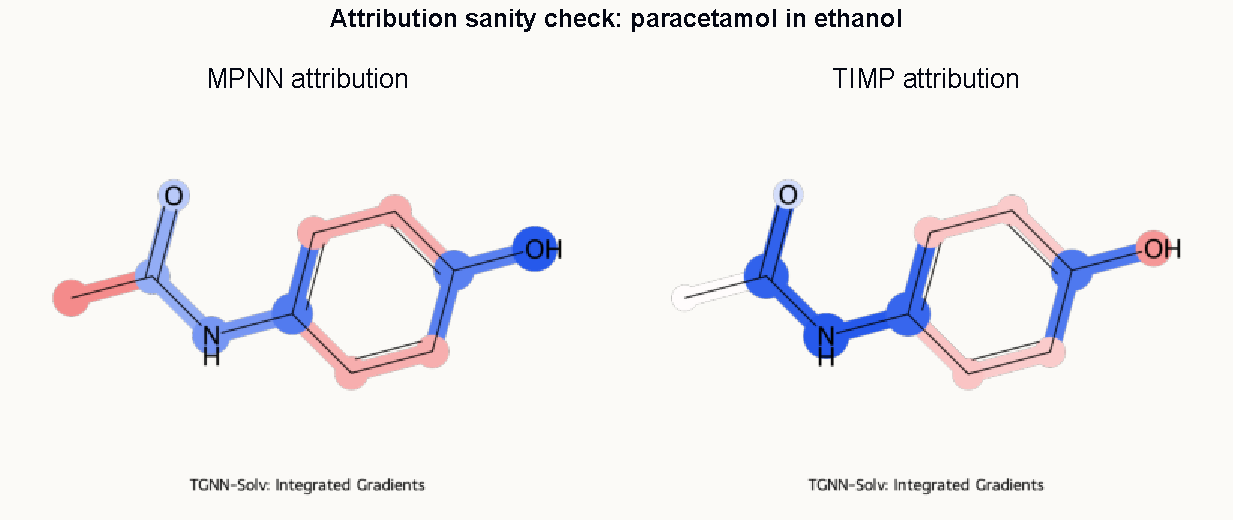
\includegraphics[width=0.92\textwidth]{attribution_examples.pdf}
\caption{Пример карт вклада атомов для пары парацетамол--этанол. Такие карты служат диагностикой здравого смысла, а не самостоятельным доказательством правильности модели.}
\label{fig:app-attribution-examples}
\end{figure}

Для прикладного использования одного числа $\widehat{\ln x_2}$ недостаточно. Нужны интервал неопределённости, флаг выхода из области применимости и химически понятные расстояния до известных примеров. Этот слой реализован, но числовая калибровка на основном тесте ещё не завершена.

\begin{figure}[!htbp]
\centering
\includegraphics[width=0.90\textwidth]{uncertainty_ad_schematic.pdf}
\caption{Слой неопределённости и области применимости сопровождает прогноз интервалом, расстоянием до обучающей области и химически понятными признаками выхода за пределы применимости.}
\label{fig:app-uncertainty-ad}
\end{figure}

Практический слой поддерживает прогноз для одной пары, температурное сканирование, ранжирование растворителей и оценку технологического окна. Эти сценарии важны для инженерной завершённости, но они не заменяют основную научную проверку: выигрывает ли физический путь у прямого предсказания при честном разбиении.

\subsection{План обязательных проверок}

Полноразмерная вычислительная серия должна быть заранее ограничена понятными критериями. Иначе легко получить ещё один общий MAE без понимания механизма. Пороговые значения ниже не являются универсальными физическими константами; это рабочий контракт для следующей серии запусков.

\begin{table}[!htbp]
\centering
\caption{Минимальный набор проверок для полноразмерного этапа.}
\label{tab:app-next-validation-contract}
\small
\begin{tabularx}{\textwidth}{P{0.26\textwidth}Y P{0.25\textwidth}}
\toprule
Проверка & Что измеряет & Критерий полезности \\
\midrule
Температурная экстраполяция, полный бюджет & Использует ли TGNN-Solv известную форму зависимости от температуры & MAE ниже DirectGNN хотя бы на $0.10$ и ошибка наклона ниже минимум на $20\%$ \\
Контрольная подстановка кристалла & Какая часть ошибки идёт от $T_m$ и $\Delta H_{\mathrm{fus}}$ & Изменение MAE не меньше $0.3$ на совпавших строках; иначе кристалл не считается главным объяснением \\
Аудит NRTL-параметров & Стали ли $\tau_{12}$, $\tau_{21}$, $\alpha$ парно-различимыми и физически ограниченными & $\sigma(\tau_{12})$ или $\sigma(\tau_{21})>0.1$, при этом менее $5\%$ значений упираются в ограничения \\
Величина остаточной коррекции & Не превратилась ли модель в прямую регрессию после решателя & Медианный модуль поправки меньше половины медианного модуля физического выхода, а MAE улучшается минимум на $0.05$ \\
Случайные пары & Есть ли чрезмерная цена физического слоя в лёгком интерполяционном режиме & Разрыв TGNN-Solv и DirectGNN по MAE не больше $0.15$ при известных компонентах пары \\
Структурные срезы и BRICS & Улучшается ли перенос на новые фрагменты и сложные химические классы & Разрыв между полностью покрытыми и преимущественно новыми фрагментами уменьшается минимум на $15\%$ \\
\bottomrule
\end{tabularx}
\end{table}

Самая важная проверка --- температурная экстраполяция при полном бюджете обучения. Именно там физическая форма уже имеет сильный ориентир: Вант-Гофф даёт $\mae=0.368$ в режиме известной пары. Если TGNN-Solv при полном обучении приблизится к этому режиму и обойдёт DirectGNN, это станет содержательным аргументом в пользу физического пути даже при близком качестве на новых каркасах.

\clearpage

\section*{Математическое обоснование}
\addcontentsline{toc}{section}{Математическое обоснование}

\section{Вывод уравнения SLE}
\label{app:sle}

Запишем химический потенциал растворённого вещества в жидкой смеси~\cite{prausnitz1998,hildebrand1970}:
\begin{equation*}
    \mu_2^{\mathrm{liq}} = \mu_2^{\mathrm{liq},0} + RT\ln a_2,
    \qquad
    a_2=\gamma_2 x_2.
\end{equation*}
В твёрдой фазе считаем вещество чистым:
\begin{equation*}
    \mu_2^{\mathrm{sol}}=\mu_2^{\mathrm{sol},0}.
\end{equation*}
В равновесии:
\begin{equation*}
    \mu_2^{\mathrm{sol},0}=\mu_2^{\mathrm{liq},0}+RT\ln(\gamma_2x_2).
\end{equation*}
Переносим члены:
\begin{equation*}
    RT\ln(\gamma_2x_2)=\mu_2^{\mathrm{sol},0}-\mu_2^{\mathrm{liq},0}
    =-\left(\mu_2^{\mathrm{liq},0}-\mu_2^{\mathrm{sol},0}\right).
\end{equation*}
По определению
\begin{equation*}
    \dGfus(T)=\mu_2^{\mathrm{liq},0}(T)-\mu_2^{\mathrm{sol},0}(T).
\end{equation*}
Следовательно,
\begin{equation*}
    \ln(\gamma_2x_2)=-\frac{\dGfus(T)}{RT},
\end{equation*}
и окончательно
\begin{equation*}
    \ln x_2=-\frac{\dGfus(T)}{RT}-\ln\gamma_2.
\end{equation*}
Это равенство является прямым следствием условия фазового равновесия при заданной модели $\gamma_2$.

\section{Свободная энергия плавления и теплоёмкостная поправка}
\label{app:fusion}

Пусть при температуре плавления $\Tm$ известна энтальпия плавления $\dHfus=\Delta H_{\mathrm{fus}}(\Tm)$~\cite{acree2010,yalkowsky1979}. По определению в точке плавления
\begin{equation*}
    \Delta G_{\mathrm{fus}}(\Tm)=0,
    \qquad
    \Delta S_{\mathrm{fus}}(\Tm)=\frac{\dHfus}{\Tm}.
\end{equation*}
Если $\dCpfus$ считать постоянной, то при температуре $T$:
\begin{align*}
    \Delta H_{\mathrm{fus}}(T)
    &= \dHfus + \dCpfus(T-\Tm), \\
    \Delta S_{\mathrm{fus}}(T)
    &= \frac{\dHfus}{\Tm}+\dCpfus\ln\frac{T}{\Tm}.
\end{align*}
Тогда
\begin{align*}
    \Delta G_{\mathrm{fus}}(T)
    &= \Delta H_{\mathrm{fus}}(T)-T\Delta S_{\mathrm{fus}}(T) \\
    &= \dHfus\left(1-\frac{T}{\Tm}\right)
       +\dCpfus\left[(T-\Tm)-T\ln\frac{T}{\Tm}\right].
\end{align*}
Делим на $RT$ и получаем выражение для кристаллического вклада:
\begin{equation}
    \Phi(T)=\frac{\Delta G_{\mathrm{fus}}(T)}{RT}
    =\frac{\dHfus}{R}\left(\frac{1}{T}-\frac{1}{\Tm}\right)
    -\frac{\dCpfus}{R}\left(\frac{\Tm-T}{T}+\ln\frac{T}{\Tm}\right).
    \label{eq:phi-dcp}
\end{equation}

\begin{estimate}[Порядок ошибки при $\Delta C_p=0$]
Пусть $\Tm=500\,\mathrm{K}$, $T=298\,\mathrm{K}$, $\dCpfus=40\,\mathrm{J\,mol^{-1}\,K^{-1}}$. Тогда
\begin{equation*}
    B=\frac{\Tm-T}{T}+\ln\frac{T}{\Tm}
    =\frac{202}{298}+\ln(0.596)\approx 0.678-0.518=0.160.
\end{equation*}
Теплоёмкостная поправка к $\ln x_2$ имеет величину
\begin{equation*}
    \frac{\dCpfus}{R}B\approx \frac{40}{8.314}\cdot 0.160\approx 0.77.
\end{equation*}
Следовательно, пренебрежение $\Delta C_p$ может давать ошибку порядка $0.5$--$0.8$ в $\ln x_2$, то есть величину, сравнимую с ожидаемым выигрышем сильных моделей.
\end{estimate}

\section{Модель NRTL и IDAC-данные}
\label{app:nrtl}

Для бинарной системы NRTL задаёт~\cite{renon1968}
\begin{equation*}
    G_{ij}=\exp(-\alpha\tau_{ij}).
\end{equation*}
Здесь индекс $1$ обозначает растворитель, индекс $2$ --- растворяемое вещество. Запись ниже является бинарной формой для $\ln\gamma_2$; она не предназначена для многокомпонентной смеси без расширения индексов. Коэффициент активности растворённого вещества записывается как
\begin{equation}
\ln\gamma_2
= x_1^2\left[
\tau_{12}\left(\frac{G_{12}}{x_2+x_1G_{12}}\right)^2
+ \frac{\tau_{21}G_{21}}{(x_1+x_2G_{21})^2}
\right].
\label{eq:nrtl}
\end{equation}
В пределе $x_2\to0$ имеем $x_1\to1$ и
\begin{equation*}
    \frac{G_{12}}{x_2+x_1G_{12}}\to 1,
    \qquad
    \frac{G_{21}}{(x_1+x_2G_{21})^2}\to G_{21}.
\end{equation*}
Поэтому
\begin{equation}
    \ln\gamma_2^{\infty}=\tau_{12}+\tau_{21}G_{21}
    =\tau_{12}+\tau_{21}\exp(-\alpha\tau_{21}).
    \label{eq:idac}
\end{equation}
Это объясняет, почему IDAC-данные дают частичный прямой сигнал на NRTL-часть модели. Они не являются метками растворимости, но ограничивают ту же ветвь активности. В области $x_2\ll1$ это прежде всего ограничение одной эффективной комбинации параметров, а не полное восстановление всей формы $\gamma_2(x,T)$.

\begin{remark}
Одна IDAC-точка не определяет три параметра $\tau_{12}$, $\tau_{21}$ и $\alpha$ однозначно. Поэтому IDAC-данные уменьшают неоднозначность, но не устраняют её полностью. Отсюда следует необходимость дополнительных сигналов: температурных рядов, UNIFAC-приоров, GE/VLE-данных и регуляризации физических диапазонов.
\end{remark}


\section{SLE как задача о неподвижной точке и неявное дифференцирование}
\label{app:implicit}

После выбора $\Phi(T)$ и параметров NRTL уравнение равновесия можно записать как
\begin{equation*}
    F(x_2)=x_2\gamma_2(x_2,T)-\exp[-\Phi(T)] = 0.
\end{equation*}
Эквивалентная логарифмическая форма удобнее для анализа:
\begin{equation*}
    H(q)=q+\ln\gamma_2(\exp q,T)+\Phi(T)=0,
    \qquad q=\ln x_2.
\end{equation*}
В коде решается не напрямую $H(q)=0$, а неподвижная точка
\begin{equation*}
    x^{(k+1)} = G(x^{(k)})
    = \exp[-\Phi(T)-\ln\gamma_2(x^{(k)},T)].
\end{equation*}
Начальное приближение выбрано как идеальная растворимость
\begin{equation*}
    x^{(0)} = \exp[-\Phi(T)],
\end{equation*}
то есть решение при $\gamma_2=1$. Такой старт имеет физический смысл: если $|\ln\gamma_2|\leq \Gamma$ и $H'(q)\geq \mu>0$ в рабочем интервале, то по теореме Лагранжа
\begin{equation*}
    |q^*-q^{(0)}|
    \leq \Gamma/\mu .
\end{equation*}
Иными словами, идеальное решение лежит на расстоянии, контролируемом только величиной неидеальности. Для большинства строк корпуса $x_2\ll1$, и член
$x_2\,\partial\ln\gamma_2/\partial x_2$ мал, $H'(q)\approx 1$, и эта оценка практически означает, что старт находится в бассейне притяжения физического корня.

\begin{figure}[!htbp]
    \centering
    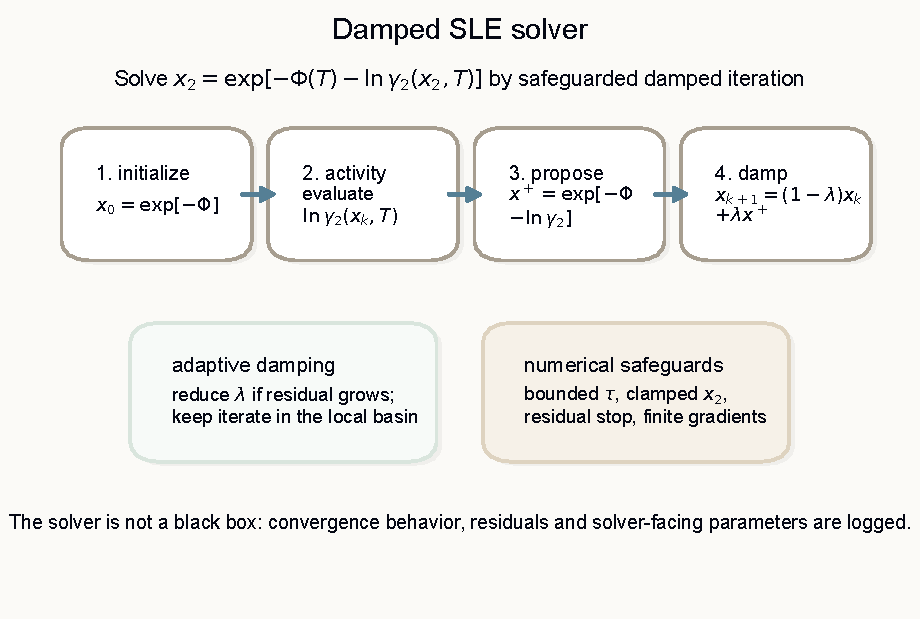
\includegraphics[width=0.96\textwidth]{figures/solver_convergence_schematic.pdf}
    \caption{Схема численного решения SLE как демпфированной итерации неподвижной точки. Все подписи на рисунке оставлены на английском языке, как и на остальных графиках отчёта.}
    \label{fig:solver-convergence-schematic}
\end{figure}

Существование решения следует из непрерывности $H(q)$ на усечённом интервале
$q\in[\ln\varepsilon,\ln(1-\varepsilon)]$. При ограниченных $\tau_{12},\tau_{21}$ и $\alpha$ коэффициент активности конечен. На левом конце $H(q)$ отрицателен за счёт $q\to-\infty$, а около $q=0$ для твёрдого вещества при $T<T_m$ обычно $\Phi(T)>0$ и $H(q)$ положителен. Корень существует по теореме о промежуточном значении. Единственность обеспечивается достаточным условием
\begin{equation*}
    H'(q)=1+x_2\frac{\partial \ln\gamma_2}{\partial x_2} \geq \mu>0.
\end{equation*}
Это условие проверяемо численно и физически естественно: в области малой растворимости $x_2$ подавляет производную активности, а NRTL-параметры в модели ограничены. Если в отдельных точках знаменатель неявной производной становится слишком мал, обратный проход дополнительно ограничивает
$|1+x_2\eta|$ снизу, где $\eta=\partial\ln\gamma_2/\partial x_2$. Это не меняет прямое предсказание, но предотвращает нефизический взрыв градиента.

Чтобы итерации не осциллировали при плохих ранних параметрах, используется демпфирование:
\begin{equation*}
    x^{(k+1)}
    =\lambda_k G(x^{(k)})+(1-\lambda_k)x^{(k)},
    \qquad 0<\lambda_k\leq 1.
\end{equation*}
Если $G'(x)$ лежит в интервале $[m,M]$ и $M<1$, то производная демпфированной карты равна
$(1-\lambda)+\lambda G'(x)$. При выборе
\begin{equation*}
    0<\lambda<\frac{2}{1-m}
\end{equation*}
она по модулю меньше единицы для отрицательных $m$, что устраняет типичную двухточечную осцилляцию. В реализации начальное $\lambda=0.7$, минимальное $0.1$; если логарифмический остаток растёт, шаг уменьшается вдвое, а если остаток падает, шаг медленно увеличивается. Поэтому демпфирование работает как локальный line-search для неподвижной точки.

Неявное дифференцирование записывается для функции~\cite{gould2021}
\begin{equation*}
    F(x_2,\theta)=x_2\gamma_2(x_2,T;\theta)-\exp[-\Phi(T)] .
\end{equation*}
По теореме о неявной функции
\begin{equation*}
    \frac{\partial x_2^*}{\partial\theta}
    =-
    \frac{\partial F/\partial\theta}{\partial F/\partial x_2}.
\end{equation*}
Так как
\begin{equation*}
    \frac{\partial F}{\partial x_2}
    =\gamma_2\left(1+x_2\frac{\partial\ln\gamma_2}{\partial x_2}\right),
\end{equation*}
то в логарифмической переменной существенный знаменатель имеет вид
$1+x_2\eta$. Именно этот множитель диагностировался как возможное узкое место градиента через физический слой.

Численная точность контролируется остатком
\begin{equation*}
    r_k=|\ln G(x^{(k)})-\ln x^{(k)}|.
\end{equation*}
В режиме сжатия с константой $L<1$ ошибка после $k$ итераций удовлетворяет стандартной оценке
\begin{equation*}
    |q_k-q^*|\leq \frac{L}{1-L}|q_k-q_{k-1}|.
\end{equation*}
Поскольку метрика отчёта сама является ошибкой в $q=\ln x_2$, эта величина напрямую измеряет вклад численного решателя в MAE. Ограничения $x_2\in[10^{-10},1-10^{-10}]$ защищают от переполнения и логарифма нуля; в выводах отчёта это означает, что численная ошибка решателя существенно меньше наблюдаемого модельного разрыва порядка $1$--$2$ в $\ln x_2$.

\section{Чувствительность к кристаллическим параметрам}
\label{app:sensitivity}

В приближении $\Delta C_p=0$ и при фиксированном $\gamma_2$:
\begin{equation*}
    \ln x_2=-\frac{\dHfus}{R}\left(\frac{1}{T}-\frac{1}{\Tm}\right)-\ln\gamma_2.
\end{equation*}
Тогда
\begin{align*}
    \frac{\partial \ln x_2}{\partial \Tm}
    &=-\frac{\dHfus}{R\Tm^2}, \\
    \frac{\partial \ln x_2}{\partial \dHfus}
    &=-\frac{1}{R}\left(\frac{1}{T}-\frac{1}{\Tm}\right).
\end{align*}

\begin{estimate}[Ошибка температуры плавления]
Пусть $\dHfus=30\,\mathrm{kJ/mol}$, $\Tm=450\,\mathrm{K}$, ошибка $\delta\Tm=30\,\mathrm{K}$. Тогда
\begin{equation*}
    \abs{\delta\ln x_2}
    \approx \frac{30000}{8.314\cdot 450^2}\cdot 30
    \approx 0.53.
\end{equation*}
Только ошибка $\Tm$ порядка $30\,\mathrm{K}$ способна дать вклад около $0.5$ в $\ln x_2$.
\end{estimate}

\begin{estimate}[Ошибка энтальпии плавления]
Пусть $T=298\,\mathrm{K}$, $\Tm=450\,\mathrm{K}$, ошибка $\delta\dHfus=5\,\mathrm{kJ/mol}$. Тогда
\begin{equation*}
    \abs{\delta\ln x_2}
    \approx \frac{5000}{8.314}\left(\frac{1}{298}-\frac{1}{450}\right)
    \approx 0.68.
\end{equation*}
Следовательно, даже умеренная ошибка $\dHfus$ может быть сопоставима с целевой ошибкой всей модели.
\end{estimate}

Эти оценки объясняют, почему физический путь может проигрывать прямой модели: ошибка промежуточных физических параметров усиливается при прохождении через уравнение равновесия.

\begin{figure}[!htbp]
\centering
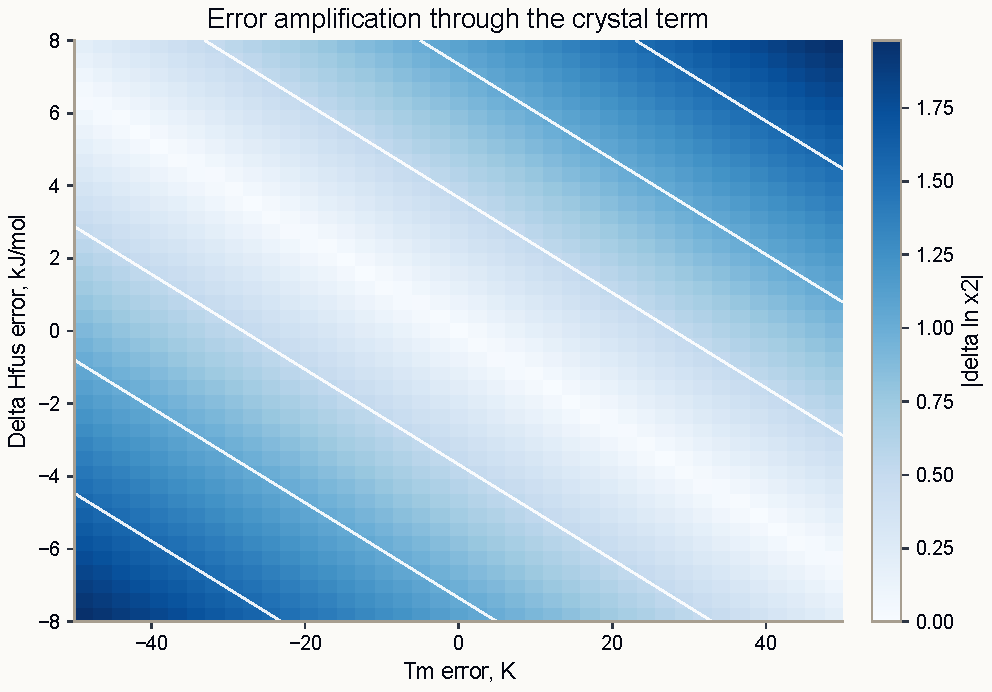
\includegraphics[width=0.84\textwidth]{sensitivity_heatmap.pdf}
\caption{Чувствительность $\ln x_2$ к ошибкам кристаллических параметров. Даже умеренные ошибки $\Tm$ и $\dHfus$ способны дать вклад того же порядка, что и весь целевой выигрыш между моделями.}
\label{fig:sensitivity-heatmap}
\end{figure}

\section{Вант-Гофф, температурные наклоны и кондиционирование}
\label{app:vant-hoff}

Если энтальпия растворения приблизительно постоянна, то
\begin{equation*}
    \frac{\partial \ln x_2}{\partial (1/T)}\approx -\frac{\Delta H_{\mathrm{sol}}}{R}.
\end{equation*}
Для одной пары линейная регрессия
\begin{equation*}
    \ln x_2 = a + b\frac{1}{T}
\end{equation*}
даёт оценку
\begin{equation*}
    \Delta H_{\mathrm{sol}}\approx -Rb.
\end{equation*}

\begin{estimate}[Физический смысл ошибки наклона]
Если ошибка наклона равна $1600\,\mathrm{K}$, то ошибка эффективной энтальпии растворения составляет
\begin{equation*}
    \abs{\delta\Delta H_{\mathrm{sol}}}
    \approx R\cdot 1600
    \approx 8.314\cdot 1600
    \approx 13.3\,\mathrm{kJ/mol}.
\end{equation*}
Это химически существенная величина, сравнимая с изменением нескольких сильных межмолекулярных контактов.
\end{estimate}

\begin{estimate}[Почему близкие температуры плохо определяют наклон]
Пусть есть три точки в узком диапазоне $298$--$310\,\mathrm{K}$. Тогда диапазон переменной $u=1/T$ равен
\begin{equation*}
    \Delta u = \frac{1}{298}-\frac{1}{310}\approx 1.30\times10^{-4}\,\mathrm{K}^{-1}.
\end{equation*}
Для трёх приблизительно равномерных точек
\begin{equation*}
    S_{uu}=\sum_i(u_i-\bar u)^2 \approx \frac{(\Delta u)^2}{2}
    \approx 8.5\times10^{-9}\,\mathrm{K}^{-2}.
\end{equation*}
Если шум $\ln x_2$ имеет стандартное отклонение всего $\sigma=0.1$, то стандартная ошибка наклона порядка
\begin{equation*}
    \mathrm{SE}(b)\approx \frac{\sigma}{\sqrt{S_{uu}}}
    \approx \frac{0.1}{9.2\times10^{-5} }
    \approx 1.1\times10^3\,\mathrm{K}.
\end{equation*}
Поэтому даже физически правильная модель может плохо восстанавливать температурный наклон, если температурный диапазон узок или измерения шумны.
\end{estimate}

\section{Идентифицируемость кристалла и активности}
\label{app:identifiability}

Линеаризуем модель по параметрам, отвечающим за температурный наклон. Упрощённо:
\begin{equation*}
    \ln x_2(T)
    \approx c_0
    -\frac{\dHfus}{R}\left(\frac{1}{T}-\frac{1}{\Tm}\right)
    -\beta_{\gamma}\left(\frac{1}{T}-\frac{1}{T_{\mathrm{ref}}}\right),
\end{equation*}
где $\beta_{\gamma}$ обозначает эффективный температурный вклад активности. Обе величины $\dHfus$ и $\beta_{\gamma}$ умножаются на функции, близкие к линейным по $1/T$. При узком температурном диапазоне столбцы соответствующей матрицы чувствительности почти коллинеарны.

Пусть вектор наблюдений $y$ аппроксимируется как
\begin{equation*}
    y\approx X\theta,\qquad
    \theta=(\dHfus,\beta_{\gamma},c_0)^\top.
\end{equation*}
Дисперсия оценки в линейной модели пропорциональна
\begin{equation*}
    \Var(\widehat\theta)\propto (X^\top X)^{-1}.
\end{equation*}
Если $X^\top X$ плохо обусловлена, малый шум в $y$ даёт большой разброс в $\widehat\theta$. Именно это и есть компенсаторная вырожденность: кристаллическая часть и активность могут взаимно поглощать ошибки друг друга, сохраняя похожее $\ln x_2$.

Отсюда следует практическое требование: одних SLE-строк недостаточно. Нужны дополнительные сигналы, которые отдельно ограничивают кристаллические свойства и активность. В проекте эту роль выполняют $\Tm$, $\dHfus$, IDAC, UNIFAC, параметры Хансена и температурные кривые.

\section{Формальная запись предобучения и функции ошибки}
\label{app:loss-pretraining}

Этап 0 можно записать как многозадачное обучение графового блока $h_\theta(G)$ на молекулярных графах без целевой растворимости:
\begin{equation*}
    \mathcal L_{\mathrm{stage0}}
    = \lambda_{\mathrm{atom}}\mathcal L_{\mathrm{atom}}
    + \lambda_{\mathrm{bond}}\mathcal L_{\mathrm{bond}}
    + \lambda_{\mathrm{desc}}\mathcal L_{\mathrm{desc}}
    + \lambda_{\mathrm{contr}}\mathcal L_{\mathrm{contr}}.
\end{equation*}
Для маскированных атомных признаков используется классификационная или смешанная классификационно-регрессионная ошибка по скрытым признакам:
\begin{equation*}
    \mathcal L_{\mathrm{atom}}
    = -\sum_{i\in M_{\mathrm{atom}}}\log p_\theta(a_i\mid G_{\setminus M}).
\end{equation*}
Для типа связи:
\begin{equation*}
    \mathcal L_{\mathrm{bond}}
    = -\sum_{(i,j)\in M_{\mathrm{bond}}}\log p_\theta(b_{ij}\mid G_{\setminus M}).
\end{equation*}
Для дескрипторов:
\begin{equation*}
    \mathcal L_{\mathrm{desc}}
    = \left\| W_{\mathrm{desc}} h_\theta(G)-d(G)\right\|_2^2,
\end{equation*}
где $d(G)$ --- нормированный вектор RDKit-дескрипторов. Контрастивная часть может быть записана в форме InfoNCE:
\begin{equation*}
    \mathcal L_{\mathrm{contr}}
    =-\log
    \frac{\exp(\operatorname{sim}(z_i,z_i^+)/\tau)}
    {\exp(\operatorname{sim}(z_i,z_i^+)/\tau)+
     \sum_j\exp(\operatorname{sim}(z_i,z_j^-)/\tau)}.
\end{equation*}
Здесь $z$ --- проекция молекулярного представления, $z_i^+$ --- другая аугментированная версия той же молекулы, $z_j^-$ --- отрицательные примеры.

Основная функция обучения TGNN-Solv после этапа 0 имеет вид
\begin{equation*}
    \mathcal L_{\mathrm{TGNN}}
    = \sum_k \lambda_k^{(p)} \mathcal L_k,
\end{equation*}
где $p$ обозначает фазу обучения. Фазовая зависимость весов не является косметической деталью: при $p=1$ доминируют кристаллические и вспомогательные свойства, при $p=2$ доминирует растворимость, при $p=3$ уменьшается шаг оптимизации и остаются физические ограничения.

Если для строки отсутствует вспомогательная метка, соответствующий член выключается маской:
\begin{equation*}
    \mathcal L_T
    = \frac{\sum_i m_i^T \rho(\widehat T_{m,i}-T_{m,i})}
           {\sum_i m_i^T+\varepsilon}.
\end{equation*}
Такой вид важен: отсутствующие физические свойства не должны превращаться в искусственные нули.

Для температурных рядов одной пары можно ввести локальное ограничение на наклон. Пусть $u=1/T$ и для пары $r$ известна оценка наклона $b_r$ из обучающих точек. Эта оценка должна вычисляться один раз до обучения и использоваться как фиксированный якорь; она не должна пересчитываться по текущим предсказаниям модели и не должна строиться по валидационным или тестовым точкам. Тогда вспомогательный член можно записать как
\begin{equation*}
    \mathcal L_{\mathrm{slope}}
    = \sum_r \rho\!\left(
        \frac{\widehat{\ln x_2}(u_{r,2})-\widehat{\ln x_2}(u_{r,1})}
             {u_{r,2}-u_{r,1}}
        - b_r
    \right),
\end{equation*}
если в мини-пакете или в специальном якорном наборе есть две температуры одной пары. Этот член напрямую проверяет то, что оказалось главной температурной проблемой запусков с малым бюджетом: восстановление физического наклона, а не только точечного значения. Его статус ограничен: это обучение внутри известной пары, а не доказательство переноса температурной физики на новую пару.

\section{Математическое обоснование предложенных доработок}
\label{app:improvements}

\subsection{Отдельный IDAC-поток}

Из \eqref{eq:idac} следует, что IDAC ограничивает комбинацию параметров NRTL. Если добавлять IDAC как обычную строку растворимости, возникает неверная постановка: у такой строки нет SLE-измерения $\ln x_2$. Поэтому корректный путь --- отдельный вспомогательный член функции обучения:
\begin{equation*}
    \mathcal L_{\mathrm{IDAC}}
    = w_{\mathrm{exp}}\,\rho\!
    \left(\widehat{\ln\gamma_2^{\infty}}-\ln\gamma_{2,\mathrm{exp}}^{\infty}\right),
\end{equation*}
где $\rho$ --- устойчивая ошибка, например Хьюбера~\cite{huber1964}. Для псевдометок UNIFAC вес должен быть меньше:
\begin{equation*}
    w_{\mathrm{UNIFAC}}<w_{\mathrm{exp}}.
\end{equation*}
В текущей серии проверок применяется отношение $0.15$ против $1.0$.

\subsection{UNIFAC как приор}

Пусть детерминированная групповая модель даёт оценку $\tau^{(0)}$ или, слабее, оценку $\ln\gamma^\infty$. Тогда нейросетевая модель может учить не полный параметр из нуля, а поправку:
\begin{equation*}
    \tau_{ij}=\tau_{ij}^{(0)}+\Delta\tau_{ij}^{\mathrm{NN}}.
\end{equation*}
Если $\tau_{ij}^{(0)}$ в среднем ближе к истинному параметру на рассматриваемом распределении, чем случайная инициализация или чисто нейросетевая экстраполяция,
\begin{equation*}
    \E\abs{\tau_{ij}^{(0)}-\tau_{ij}^{\star}}
    <
    \E\abs{\tau_{ij}^{\mathrm{NN}}-\tau_{ij}^{\star}},
\end{equation*}
то задача обучения поправки проще:
\begin{equation*}
    \E\abs{\Delta\tau_{ij}^{\mathrm{NN}}}
    < \E\abs{\tau_{ij}^{\mathrm{NN}}}.
\end{equation*}
Это и есть смысл приора: он не обязан быть точным, но должен уменьшать радиус поиска для параметров активности. Для новых каркасов это является допущением, а не гарантией; ограниченное покрытие UNIFAC означает, что плохой приор должен иметь малый вес и не должен доминировать над экспериментальными SLE- и IDAC-сигналами.

\subsection{Градиентное голодание перекрёстного внимания}
\label{app:cross-attention-starvation}

Перекрёстное внимание строит парное представление: атомы растворяемого вещества получают информацию от атомов растворителя и наоборот. Именно это представление затем должно нести информацию о совместимости пары и питать NRTL-голову. Слабый градиент в этом блоке является более точной диагностикой, чем общий тезис «физическая модель плохо обучается».

В диагностическом прогоне сравнивались нормы градиента в TGNN-Solv и DirectGNN. Картина оказалась асимметричной: ранний слой энкодера TGNN-Solv получал даже больший сигнал, чем DirectGNN, но попарное перекрёстное внимание получало примерно в $33$ раза меньший градиент:
\begin{equation*}
    \frac{\|\nabla_{\mathrm{attn}}\mathcal L_{\mathrm{TGNN}}\|}
         {\|\nabla_{\mathrm{attn}}\mathcal L_{\mathrm{Direct}}\|}
    \approx
    \frac{0.0007}{0.023}
    \approx 0.03.
\end{equation*}
Это означает, что проблема не в полном исчезновении градиента, а в неправильном маршруте обучения. Общий энкодер получает сигнал через кристаллические свойства одиночной молекулы, а блок, который должен учить контакты «вещество--растворитель», остаётся слабее обученным.

Исправление проверяет именно этот механизм. Вспомогательная ветка
\begin{equation*}
    \mathbf g_{\mathrm{pair}}
    \rightarrow f_{\mathrm{aux}}
    \rightarrow \ln x_2^{\mathrm{aux}}
\end{equation*}
добавляет малую ошибку Хьюбера по растворимости только во время обучения. В проверочной постановке использовалась фазовая логика весов $0 \to 0.1 \to 0.01$: в первой фазе ветка выключена, во второй оживляет парный блок, в третьей не должна доминировать над физическим путём. Отдельно рассматривается отсечение кристаллического градиента:
\begin{equation*}
    \mathbf g_{\mathrm{sol}}^{\mathrm{crystal}}
    =
    \operatorname{sg}(\mathbf g_{\mathrm{sol}}),
\end{equation*}
где $\operatorname{sg}$ означает остановку градиента. Тогда кристаллическая голова продолжает обучаться, но перестаёт переписывать общий энкодер сильнее, чем ветвь взаимодействия.

Короткая проверка на $50$ шагах показала, что вспомогательная ветка действительно восстанавливает поток градиента: норма градиента попарного внимания стала $0.0377$ против $0.0381$ у DirectGNN. Это почти равный масштаб. Повторная малая проверка в режиме прямого предела активности дала более осторожную картину: одно отсечение кристаллического градиента оставило отношение парного сигнала к DirectGNN около $0.069$, а добавление вспомогательной парной потери с весом $0.2$ подняло его до $0.268$. Дополнительная проверка веса показала сильную зависимость: $0.5$ даёт отношение около $0.667$, а $1.0$ --- около $1.33$. Отсечение кристаллических параметров от SLE-градиента при весе $0.2$ почти не меняет отношение. Значит, новая параметризация активности сама по себе не решает проблему маршрута градиента, а вес прямого парного сигнала становится отдельным гиперпараметром. Отдельный малый прогон с весом $0.5$ и обучаемым смещением активности дал лишь слабое улучшение MAE ($3.236\to3.225$), хотя улучшил $R^2$. Зато тот же режим с хвостовой функцией потерь снизил MAE до $2.862$. Следовательно, восстановление градиента необходимо, но недостаточно: ему нужна функция потерь, которая не позволяет модели безопасно сжимать весь диапазон к центру. В таблицах качества такая ветка должна считаться отдельной абляцией, а не уже подтверждённым полноразмерным улучшением модели.

\begin{figure}[!htbp]
\centering
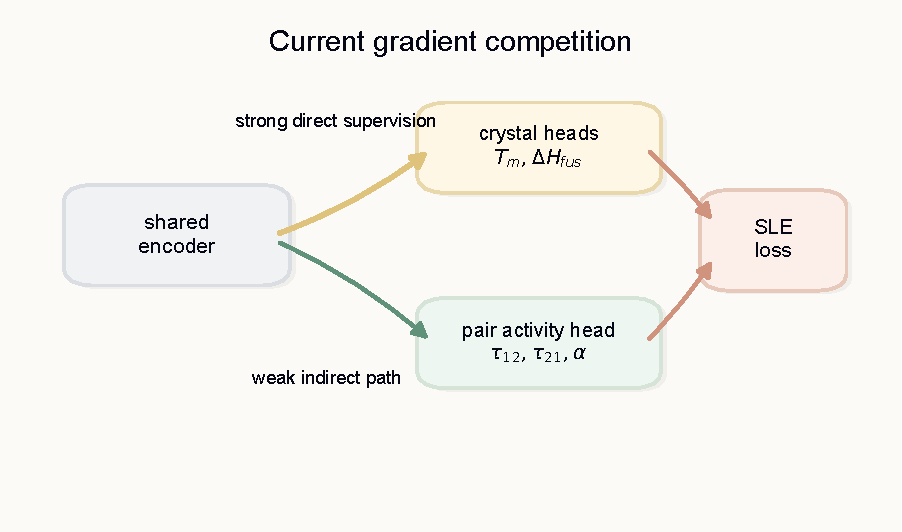
\includegraphics[width=0.88\textwidth]{gradient_flow.pdf}
\caption{Диагностика голодания перекрёстного внимания. Энкодер TGNN-Solv получает градиент, но блок парного взаимодействия получает сигнал существенно слабее, чем аналогичный блок DirectGNN.}
\label{fig:cross-attention-starvation}
\end{figure}

\begin{figure}[!htbp]
\centering
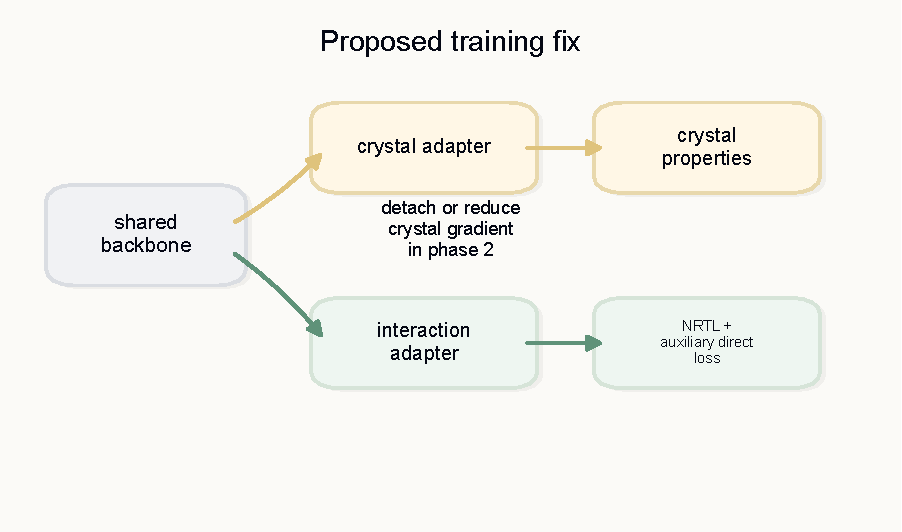
\includegraphics[width=0.88\textwidth]{gradient_flow_fix.pdf}
\caption{Проверка исправления: вспомогательная ветка на парном представлении используется только при обучении и восстанавливает градиент перекрёстного внимания до масштаба DirectGNN в коротком диагностическом прогоне.}
\label{fig:cross-attention-starvation-fix}
\end{figure}

\FloatBarrier

\subsection{Разделение кристаллической и парной информации}

Пусть общий графовый блок имеет параметры $\theta$. Тогда градиент общей функции обучения имеет вид
\begin{equation*}
    \nabla_\theta \mathcal L
    =\lambda_c\nabla_\theta\mathcal L_{\mathrm{crystal}}
    +\lambda_a\nabla_\theta\mathcal L_{\mathrm{activity}}
    +\lambda_s\nabla_\theta\mathcal L_{\mathrm{SLE}}.
\end{equation*}
Если $\mathcal L_{\mathrm{crystal}}$ имеет гораздо больше прямых меток и меньший шум, то этот градиент может доминировать. Но признаки, полезные для $\Tm$ и упаковки кристалла, не обязаны совпадать с признаками, полезными для жидкофазной совместимости пары.

Родственный, но более общий возможный механизм --- конфликт направлений градиента. Если
\begin{equation*}
    \cos\angle(\nabla\mathcal L_{\mathrm{crystal}},\nabla\mathcal L_{\mathrm{activity}})<0
\end{equation*}
или близок к нулю, общий блок получает компромиссный сигнал. В текущей работе этот угол не измерен напрямую; разделение представлений остаётся мотивированной гипотезой, а не диагностированным фактом. Для проверки нужно логировать нормы градиентов и проекции $\nabla\mathcal L_{\mathrm{crystal}}$ на $\nabla\mathcal L_{\mathrm{activity}}$ по эпохам.

\subsection{Парные параметры Хансена}

В теории параметров растворимости вклад смешения часто приближённо связан с квадратом расстояния между параметрами растворителя и растворённого вещества~\cite{hansen2007}:
\begin{equation*}
    \Delta E_{\mathrm{mix}} \propto
    (\delta_{d,2}-\delta_{d,1})^2+
    (\delta_{p,2}-\delta_{p,1})^2+
    (\delta_{h,2}-\delta_{h,1})^2.
\end{equation*}
Поэтому предсказывать только индивидуальные параметры недостаточно; важна именно разность или расстояние пары. Отсюда следует дополнительная функция обучения
\begin{equation*}
    \mathcal L_{\Delta HSP}
    =\left\|\widehat{\boldsymbol\delta_2-\boldsymbol\delta_1}
    -(\boldsymbol\delta_2-\boldsymbol\delta_1)\right\|_2^2.
\end{equation*}
Она напрямую обучает представление совместимости, а не только свойства отдельных молекул.

\subsection{Парное контрастивное предобучение}

Растворимость является парным свойством. Поэтому предобучение только на одиночных молекулах не учит совместимость. Для одного растворителя можно строить пары растворяемых веществ $A$ и $B$ и задавать метку
\begin{equation*}
    y_{AB}=\mathbb I\{\abs{\overline{\ln x_2(A)}-\overline{\ln x_2(B)}}<\varepsilon\}.
\end{equation*}
Тогда модель учит, какие вещества имеют похожую растворимость в одном и том же растворителе. Особенно важны трудные отрицательные примеры:
\begin{equation*}
    \mathrm{Tanimoto}(A,B)>0.6,
    \qquad
    \abs{\Delta\ln x_2}>2.0.
\end{equation*}
Такие пары показывают, что структурная похожесть не всегда означает близкую растворимость. После обновления генерации получено $6\,602$ парных примера: $208$ трудных отрицательных, $239$ простых положительных и $6\,155$ простых отрицательных. Это уже пригодно для вспомогательного предобучения парного представления, но само по себе не является результатом качества: нужно проверить, улучшает ли такая задача перенос на новые каркасы при том же основном протоколе.

\section{Распространение ошибки через физический слой}
\label{app:error-propagation}

Пусть физическая модель задаёт отображение
\begin{equation*}
    \widehat y
    = f(\widehat \theta_c,\widehat \theta_a; T),
    \qquad
    y=\ln x_2,
\end{equation*}
где $\theta_c=(\Tm,\dHfus,\dCpfus,\ldots)$ --- кристаллические параметры, а $\theta_a=(\tau_{12},\tau_{21},\alpha,\ldots)$ --- параметры активности. В первом порядке ошибка предсказания равна
\begin{equation}
    \delta y
    \approx
    \nabla_{\theta_c}f^\top \delta\theta_c
    +
    \nabla_{\theta_a}f^\top \delta\theta_a.
    \label{eq:error-propagation}
\end{equation}
Для прямой модели аналогичного физического разложения нет: она сразу аппроксимирует $y$. Поэтому физическая модель может проигрывать прямой даже при правильной структуре уравнения, если ошибки промежуточных параметров велики.

В простом приближении $\Delta C_p=0$ и фиксированной активности
\begin{equation*}
    f(\theta_c,\theta_a;T)
    =
    -\frac{\dHfus}{R}\left(\frac{1}{T}-\frac{1}{\Tm}\right)
    -\ln\gamma_2.
\end{equation*}
Тогда вклад кристаллических ошибок:
\begin{equation*}
    \delta y_c
    \approx
    -\frac{\dHfus}{R\Tm^2}\delta \Tm
    -
    \frac{1}{R}\left(\frac{1}{T}-\frac{1}{\Tm}\right)\delta \dHfus.
\end{equation*}
Подставляя типичные значения $\dHfus=30\,\mathrm{kJ/mol}$, $\Tm=450\,\mathrm K$, $T=298\,\mathrm K$, получаем:
\begin{align*}
    \delta \Tm=30\,\mathrm K
    &\Rightarrow
    \abs{\delta y_T}\approx 0.53,\\
    \delta \dHfus=5\,\mathrm{kJ/mol}
    &\Rightarrow
    \abs{\delta y_H}\approx 0.68.
\end{align*}
Эти два вклада уже могут дать ошибку порядка $1$ в $\ln x_2$ до учёта активности.

Для активности в первом порядке:
\begin{equation*}
    \delta y_a=-\delta\ln\gamma_2.
\end{equation*}
Если NRTL-блок ошибается в $\ln\gamma_2$ всего на $0.5$--$1.0$, итоговая ошибка становится сравнимой с наблюдаемой разницей между сильными моделями. Поэтому физическая модель требует не просто правильного уравнения, а точного обучающего сигнала для промежуточных параметров.

\begin{figure}[!htbp]
\centering
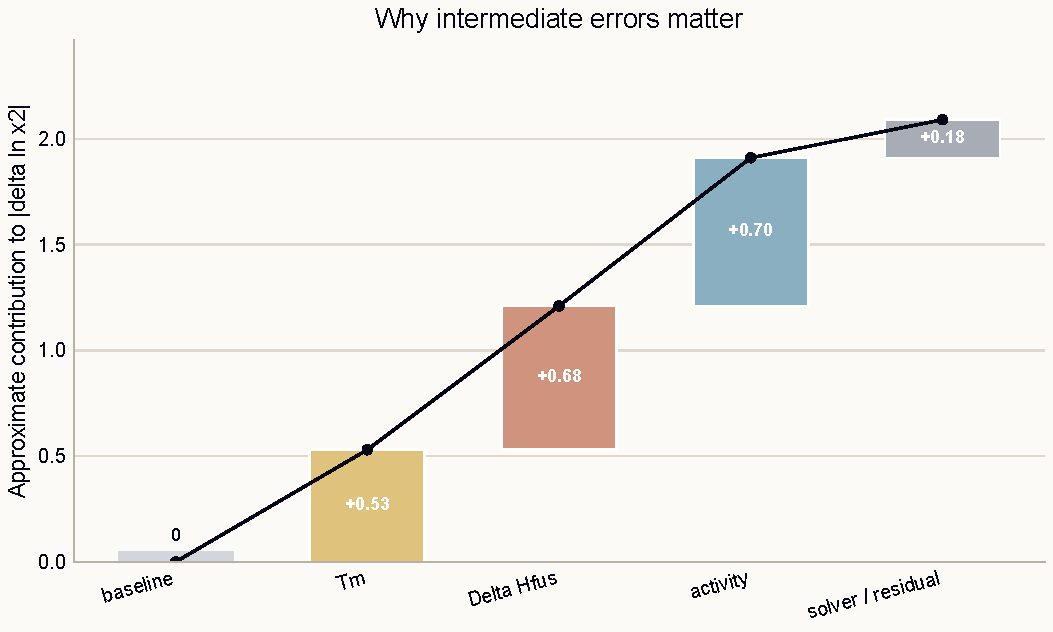
\includegraphics[width=0.84\textwidth]{error_decomposition_waterfall.pdf}
\caption{Схематическое распространение ошибок через физический слой. В TGNN-Solv ошибка промежуточных физических параметров может усиливаться до ошибки в $\ln x_2$, поэтому физическая корректность уравнения сама по себе не гарантирует низкий MAE.}
\label{fig:error-waterfall}
\end{figure}

\begin{estimate}[Иллюстрация масштаба ошибки]
Если промежуточные параметры физической модели имеют ошибку масштаба, указанного выше, то физический слой может дать больший MAE, чем прямая модель, даже если уравнение SLE термодинамически корректно. Эта оценка опирается на линейное приближение \eqref{eq:error-propagation}: при типичных параметрах ошибка $30\,\mathrm K$ в $\Tm$ даёт вклад около $0.53$, ошибка $5\,\mathrm{kJ/mol}$ в $\dHfus$ --- около $0.68$. Эти величины аддитивны только в первом порядке и надёжны лишь в окрестности рассматриваемых параметров. Если $\widehat\theta$ далеко от $\theta^\star$, например в начале обучения или на новом каркасе, линейное приближение может давать неверный масштаб и даже неверный локальный знак чувствительности.
\end{estimate}

\section*{Планируемые доработки}
\addcontentsline{toc}{section}{Планируемые доработки}

\section{Одноатомный граф воды и почему явные водороды обоснованы}
\label{app:water}

В стандартной молекулярной графовой постановке водороды часто удаляются~\cite{landrum2024,gilmer2017}. Тогда вода, записанная как SMILES \code{O}, имеет один тяжёлый атом и ноль обычных связей между тяжёлыми атомами. В реализации без самопетель, виртуальных рёбер и явных водородных рёбер множество соседей такого узла пусто. Для слоя передачи сообщений вида
\begin{equation*}
    h_i^{(\ell+1)}
    =
    U_\ell\!\left(
        h_i^{(\ell)},
        \sum_{j\in\mathcal N(i)}
        M_\ell(h_i^{(\ell)},h_j^{(\ell)},e_{ij})
    \right)
\end{equation*}
у воды множество соседей пусто: $\mathcal N(i)=\varnothing$. Поэтому
\begin{equation*}
    h_O^{(\ell+1)}=U_\ell(h_O^{(\ell)},0).
\end{equation*}
Модель может использовать начальные признаки кислорода, но не может передавать информацию по O--H связям, потому что этих рёбер нет в графе.

Если добавить явные водороды для малых молекул, вода становится графом
\begin{equation*}
    \mathrm{H{-}O{-}H}.
\end{equation*}
Тогда появляются O--H рёбра, и полярность связи, донорно-акцепторные свойства и физические признаки ребра могут участвовать в передаче сообщений. Это особенно важно для TIMP-подобных каналов, где дисперсионная и полярная части зависят от признаков рёбер.

\begin{figure}[!htbp]
\centering
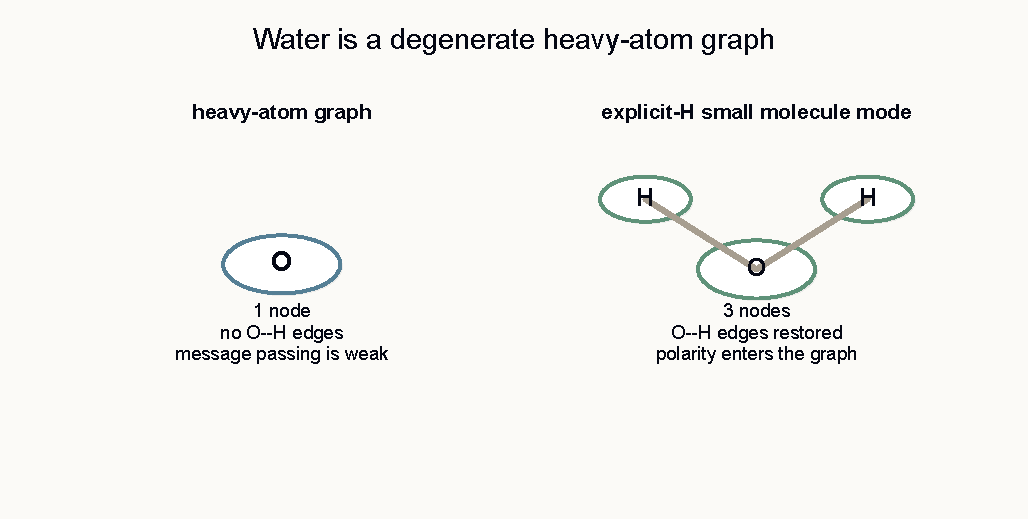
\includegraphics[width=0.88\textwidth]{water_graph_schematic.pdf}
\caption{Исправление графа воды и малых молекул: явные водороды возвращают O--H связи в граф и дают модели доступ к полярной структуре молекулы.}
\label{fig:water-graph-appendix}
\end{figure}

Эта модификация имеет химическое основание. Она восстанавливает связи, которые были удалены ради стандартной графовой экономии, но для воды и других малых молекул содержат основную физическую информацию.

\section{Статистическая интерпретация разрыва TGNN-Solv и DirectGNN}
\label{app:statistics}

Текущий разрыв на тесте по новым каркасам равен
\begin{equation*}
    \Delta_{\mathrm{MAE}}
    =
    \mae_{\mathrm{TGNN}}-\mae_{\mathrm{Direct}}
    =
    1.741-1.652
    =
    0.089.
\end{equation*}
Этот разрыв мал по сравнению с абсолютным уровнем ошибки, но он получен на согласованных предсказаниях и содержателен как диагностическая величина. Для строки $i$ определим парную разность абсолютных ошибок:
\begin{equation*}
    d_i
    =
    \abs{\widehat y_i^{\mathrm{TGNN}}-y_i}
    -
    \abs{\widehat y_i^{\mathrm{Direct}}-y_i}.
\end{equation*}
Тогда
\begin{equation*}
    \Delta_{\mathrm{MAE}}=\frac{1}{n}\sum_{i=1}^n d_i.
\end{equation*}
Положительное значение означает проигрыш TGNN-Solv по средней абсолютной ошибке. При этом TGNN-Solv лучше DirectGNN примерно на $46.4\%$ строк. Распределение $d_i$ не имеет одного знака: физическая модель выигрывает почти на половине строк, но проигрывает сильнее или чаще на оставшейся части.

Из этого следуют два вывода.

\begin{enumerate}
    \item Нельзя делать вывод только по одной общей MAE: нужна диагностика срезов, потому что модели дополняют друг друга.
    \item Для публикационного вывода при таком малом разрыве требуются несколько случайных инициализаций и парные статистические проверки.
\end{enumerate}

Корректная проверка на нескольких случайных инициализациях должна рассматривать для каждой случайной инициализации величину
\begin{equation*}
    \Delta_s
    =
    \mae_{\mathrm{TGNN},s}
    -
    \mae_{\mathrm{Direct},s}.
\end{equation*}
После этого проверяется среднее $\bar\Delta$ и доверительный интервал. Три случайные инициализации дают только предварительную проверку знака: при межзапусковой дисперсии MAE масштаба $0.1$--$0.2$ интервал остаётся слишком широким для уверенного вывода. Практический минимум для такого сравнения --- $5$--$7$ инициализаций, а публикационный вывод требует парной проверки по одинаковым разбиениям и одинаковым наборам случайных зёрен. Без таких повторов нельзя отделить устойчивый эффект физического ограничения от вариации обучения.

\section{Почему структурная экстраполяция труднее температурной}
\label{app:structural-vs-temperature}

Температурная экстраполяция внутри одной пары и структурная экстраполяция на новый каркас являются разными задачами~\cite{hildebrand1970,apelblat1999,vermeire2022}.

Внутри одной пары функциональная форма зависимости от температуры приближённо известна:
\begin{equation*}
    \ln x_2(T) \approx a+b\frac{1}{T}.
\end{equation*}
После оценки $a$ и $b$ по нескольким точкам задача становится двумерной регрессией с сильным физическим ограничением. Поэтому Вант-Гофф даёт $\mae=0.368$ в режиме известной пары.

Для нового каркаса неизвестны сами параметры пары:
\begin{equation*}
    (\tau_{12},\tau_{21},\alpha)
    =
    F(\mathrm{solute},\mathrm{solvent}).
\end{equation*}
Физика задаёт форму SLE-уравнения, но не сообщает значения $F$ для новой химической области. Структурная экстраполяция всё равно требует хорошего химического представления и переносимых приоров. Это объясняет, почему физика может быть очень сильной по температуре и одновременно не давать автоматического выигрыша на новых каркасах.

Формально можно записать ошибку на новом каркасе как сумму двух частей:
\begin{equation*}
    \abs{\widehat y-y}
    \le
    \underbrace{\abs{f(\widehat\theta,T)-f(\theta^\star,T)}}_{\text{ошибка параметров}}
    +
    \underbrace{\abs{f(\theta^\star,T)-y}}_{\text{ошибка физической модели}}.
\end{equation*}
Даже если второй член мал, первый может быть большим, если сеть плохо предсказывает параметры активности для новой химии. Расширение IDAC, UNIFAC-приоры, парное предобучение и раздельные представления кристалла/взаимодействия нужны именно для уменьшения первого члена.

\section{Связь параметров Хансена с парной совместимостью}
\label{app:hansen}

Параметры Хансена раскладывают энергию когезии на дисперсионный, полярный и водородно-связанный вклады~\cite{hansen2007}:
\begin{equation*}
    \boldsymbol\delta
    =
    (\delta_d,\delta_p,\delta_h).
\end{equation*}
Расстояние совместимости часто записывается в виде
\begin{equation*}
    R_a^2
    =
    4(\delta_{d,2}-\delta_{d,1})^2
    +(\delta_{p,2}-\delta_{p,1})^2
    +(\delta_{h,2}-\delta_{h,1})^2.
\end{equation*}
Чем меньше $R_a$, тем ближе вещества по параметрам растворимости и тем выше ожидаемая совместимость, при прочих равных условиях. Вспомогательная задача должна учить не только отдельные $\boldsymbol\delta_1$ и $\boldsymbol\delta_2$, но и их разность:
\begin{equation*}
    \mathcal L_{\mathrm{Hansen}\Delta}
    =
    \left\|
    \widehat{(\boldsymbol\delta_2-\boldsymbol\delta_1)}
    -
    (\boldsymbol\delta_2-\boldsymbol\delta_1)
    \right\|_2^2.
\end{equation*}
Это согласуется с физической целью: модель должна кодировать совместимость пары, а не только свойства отдельных молекул.



\section{TIMP: физическая декомпозиция передачи сообщений}
\label{app:timp-math}

Обычная графовая сеть передаёт одно сообщение по каждому ребру. Для растворимости это слишком грубо: вклад дисперсионных взаимодействий и вклад полярных взаимодействий имеют разную физическую природу и по-разному связаны с параметрами растворимости. В варианте TIMP сообщение раскладывается на два канала \cite{gilmer2017,gasteiger2020,hansen2007}:
\begin{equation*}
    \mathbf m_{ij}
    =
    \mathbf m_{ij}^{\mathrm{disp}}
    +
    \mathbf m_{ij}^{\mathrm{polar}} .
\end{equation*}
Дисперсионный канал соответствует лондоновскому члену $E_{\mathrm{disp}}\sim-C_6/r^6$. Для атомов $i,j$ коэффициент $C_6$ растёт с поляризуемостью; естественный масштаб сообщения задаётся как
\begin{equation*}
    s_{ij}^{\mathrm{disp}}
    =\sqrt{\alpha_i^{\mathrm{pol}}\alpha_j^{\mathrm{pol}}},
    \qquad
    \mathbf m_{ij}^{\mathrm{disp}}
    =s_{ij}^{\mathrm{disp}}\,\phi_{\mathrm d}
    (\mathbf h_i,\mathbf h_j,\mathbf e_{ij}).
\end{equation*}
Полярный канал, наоборот, должен реагировать на перераспределение заряда, различие электроотрицательностей и способность к водородным связям. В реализации это задаётся через физические признаки ребра: разность электроотрицательностей, разность ван-дер-ваальсовых радиусов, полярность связи, донорно-акцепторную маску и сложенные в тяжёлый атом заряды Гастайгера:
\begin{equation*}
    \mathbf m_{ij}^{\mathrm{polar}}
    =s_{ij}^{\mathrm{polar}}\,\phi_{\mathrm p}
    (\mathbf h_i,\mathbf h_j,\mathbf e_{ij}^{\mathrm{phys}}),
\end{equation*}
где $s_{ij}^{\mathrm{polar}}$ является гладкой положительной функцией зарядовой и донорно-акцепторной совместимости. Вектор атома обновляется суммой сообщений:
\begin{equation*}
    \mathbf h_i^{(\ell+1)}
    =U\!\left(
    \mathbf h_i^{(\ell)},
    \sum_{j\in\mathcal N(i)}
    [\mathbf m_{ij}^{\mathrm{disp}}\Vert \mathbf m_{ij}^{\mathrm{polar}}]
    \right).
\end{equation*}

Смысл этой конструкции виден через параметры Хансена. Компонента $\delta_d$ отвечает главным образом за дисперсионные взаимодействия, а $\delta_p$ и $\delta_h$ --- за полярность и водородные связи. Для TIMP введена канальная вспомогательная задача:
\begin{equation*}
    \mathcal L_{\mathrm{TIMP}}
    =
    \mathcal D(\mathbf g^{\mathrm{disp}},\delta_d)
    +
    \mathcal D(\mathbf g^{\mathrm{polar}},(\delta_p,\delta_h))
    +
    \lambda_{\perp}
    \left|
    \cos(\bar{\mathbf g}^{\mathrm{disp}},\bar{\mathbf g}^{\mathrm{polar}})
    \right| .
\end{equation*}
Здесь $\mathcal D$ --- попарное выравнивание расстояний в пространстве скрытых представлений и в пространстве физических параметров. Оно не заставляет сеть точно предсказывать параметры Хансена в каждой точке; оно требует более слабого и более полезного свойства: если две молекулы близки по дисперсионному параметру, их дисперсионные векторные представления должны быть близки, и аналогично для полярного канала.

\begin{figure}[!htbp]
    \centering
    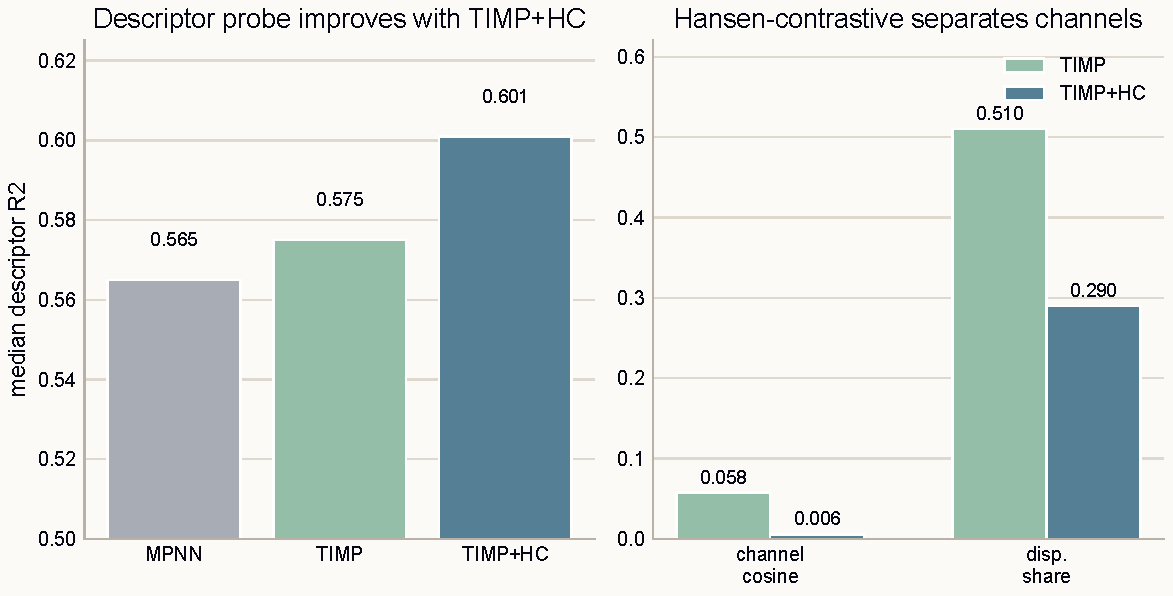
\includegraphics[width=0.86\textwidth]{figures/timp_hansen_diagnostics.pdf}
    \caption{Диагностика TIMP и контрастивного выравнивания по параметрам Хансена. Результат важен не как финальная метрика растворимости, а как проверка того, что каналы действительно кодируют разные физические свойства.}
    \label{fig:timp-hansen-appendix}
\end{figure}

Физическая связь с NRTL состоит в том, что
\begin{equation*}
    \tau_{ij}(T)=\frac{\Delta g_{ij}(T)}{RT}
\end{equation*}
является безразмерной локальной энергией контакта. В этой энергии смешаны дисперсия, полярность, водородные связи, стерическое окружение и размер молекулы. TIMP не делает NRTL более сложным, но даёт NRTL-блоку более разложенное представление пары. Это особенно важно для структурной экстраполяции: новый каркас может быть неизвестен целиком, но его дисперсионные и полярные фрагменты часто уже встречались в обучении.

Ограничения TIMP также важны. Модель остаётся двумерной графовой моделью: она не видит явные конформации, упаковку растворителя и трёхмерную сетку водородных связей. Поэтому TIMP следует рассматривать не как замену 3D-моделированию, а как физически более аккуратный способ передать в графовую сеть те признаки, которые доступны из SMILES и RDKit.

\section{Почему используется NRTL и как сохраняется термодинамическая консистентность}
\label{app:nrtl-choice-gd}

Для бинарной неидеальной жидкости нужен слой, который одновременно достаточно гибок, дифференцируем и термодинамически согласован. Wilson-модель компактна и полезна для многих жидких систем~\cite{wilson1964}, но менее удобна для задач, где нужна гибкая асимметрия локальной неслучайности и потенциальное описание сильной неидеальности. UNIQUAC физически богаче~\cite{abrams1975}, но требует надёжных объёмных и поверхностных параметров и усложняет идентифицируемость. UNIFAC хорош как группово-вкладный ориентир, но покрывает не все новые молекулы и функциональные группы. NRTL занимает промежуточное место: она явно моделирует локальную неслучайность, имеет небольшое число параметров и задаёт коэффициенты активности из единой функции избыточной свободной энергии \cite{renon1968,prausnitz1998}.

Последний пункт важен. Для бинарной смеси при фиксированных $T,P$ уравнение Гиббса--Дюгема требует
\begin{equation*}
    x_1\,d\ln\gamma_1+x_2\,d\ln\gamma_2=0 .
\end{equation*}
Если коэффициенты активности получены как производные одной молярной избыточной свободной энергии $g^E$,
\begin{equation*}
    \ln\gamma_i
    =
    \left(\frac{\partial (n g^E/RT)}{\partial n_i}\right)_{T,P,n_{j\ne i}},
\end{equation*}
то согласованность следует из однородности $n g^E$ по числам молей. NRTL удовлетворяет этому требованию: $\ln\gamma_1$ и $\ln\gamma_2$ вычисляются не независимыми нейросетями, а из общего набора $\tau_{12},\tau_{21},\alpha$.

В TGNN-Solv нейросеть предсказывает параметры NRTL, но не нарушает эту структуру. Слой активности остаётся термодинамически согласованным. Это отличие от прямой модели: DirectGNN может быть точной по MAE, но у неё нет встроенного аналога уравнения Гиббса--Дюгема. При этом для малорастворимых SLE-строк данные в основном видят область $x_2\ll1$, то есть эффективный предел $\ln\gamma_2^\infty$ и его температурную зависимость. Текущие результаты нельзя трактовать как точное восстановление индивидуальных NRTL-параметров пары. Поправочный блок TGNN-Solv также устроен через изменение физических параметров и повторное решение SLE, а не через произвольный сдвиг $\ln x_2$; благодаря этому корректировка остаётся ближе к термодинамической форме модели.

\section{Приоры, принудительная подстановка и коррекция ошибки в пространстве параметров}
\label{app:priors-teacher-correction}

В проекте используется общий принцип: если существует слабая физическая оценка $p(x)$, модель не должна заново учить абсолютное значение, а должна учить ограниченную поправку:
\begin{equation*}
    \hat y=p(x)+b\tanh r_\theta(x),
    \qquad |\hat y-p(x)|\leq b .
\end{equation*}
Так устроены кристаллические группово-вкладные приоры~\cite{joback1987,marrero2001}. Для $T_m$ поправка аддитивна, для $\Delta H_{fus}$ --- мультипликативна:
\begin{equation*}
    \widehat T_m=T_m^{\mathrm{GC}}+b_T\tanh r_T,
    \qquad
    \widehat{\Delta H}_{fus}=\Delta H_{fus}^{\mathrm{GC}}\,s(r_H),
\end{equation*}
где $s(r_H)$ ограничена заданным интервалом множителей. Последний слой остаточных ветвей инициализируется нулями; на старте модель точно равна приору. Раннее замораживание остаточных ветвей делает обучение в первой фазе похожим на калибровку, а не на немедленное разрушение физической оценки.

Для NRTL есть два более слабых источника априорной информации. Первый --- групповая Hansen-подобная априорная оценка: по счётчикам фрагментов строятся грубые $\delta_d,\delta_p,\delta_h$ и молярные объёмы, затем из расстояния $R_a$ формируется небольшой сдвиг $\tau_{12},\tau_{21}$. Второй --- UNIFAC-подобная априорная оценка по $\ln\gamma^\infty$: при малых симметричных $\tau$ приближение NRTL даёт
\begin{equation*}
    \ln\gamma_2^\infty
    =\tau_{21}+\tau_{12}\exp(-\alpha\tau_{12})
    \approx 2\tau.
\end{equation*}
Это позволяет перевести внешнюю оценку $\ln\gamma^\infty$ в слабое начальное смещение $\tau\approx\frac12\ln\gamma^\infty$. В реализации этот сдвиг ограничен, чтобы плохая внешняя априорная оценка не могла доминировать над данными.

Стохастическая подстановка истинных значений --- это разновидность принудительной подстановки для физического слоя. Если в строке есть экспериментальное $T_m$ или $\Delta H_{fus}$, то в обучении с вероятностью $p_e$ в решатель передаётся истинное значение, а не предсказание выходного блока:
\begin{equation*}
    \theta_{\mathrm{solver}}
    =M\theta_{\mathrm{exp}}+(1-M)\theta_\theta,
    \qquad M\sim\mathrm{Bernoulli}(p_e).
\end{equation*}
Это решает оптимизационную проблему: ветвь NRTL начинает видеть более правдоподобный кристаллический вклад и получает менее шумный градиент. При этом непосредственные предсказания кристаллического выходного блока остаются в выходе модели и продолжают штрафоваться собственными компонентами функции ошибки. Во второй фазе вероятность такой подстановки держится на базовом уровне, а в последние $\min(50,n_{\mathrm{epochs}})$ эпох линейно убывает до нуля:
\begin{equation*}
    p_e=p_0\left(1-
    \frac{e-e_0+1}{n_{\mathrm{anneal}}}
    \right)_+ .
\end{equation*}
В третьей фазе подстановка отключена. Поэтому финальная модель не зависит от истинных значений при применении.

Поправочный блок не добавляет произвольную прямую регрессию. Он строит новое состояние параметров
\begin{equation*}
    \theta' = \theta + \Delta\theta,
    \qquad
    |\Delta T_m|\leq 60\,\mathrm K,
    \quad
    |\Delta \Delta H/\Delta H|\leq0.25,
    \quad
    |\Delta\tau_{ij}|\leq2,
\end{equation*}
после чего SLE решается повторно. Если $q(\theta)=\ln x_2$ --- решение физического слоя, то в первом порядке
\begin{equation*}
    q(\theta')-q(\theta)
    \approx
    J_\theta\Delta\theta,
    \qquad
    J_\theta=\frac{\partial q}{\partial\theta}.
\end{equation*}
Поправочный блок является ограниченным шагом по параметрам. Он может компенсировать малые ошибки $T_m$, $\Delta H_{fus}$ и $\tau$, но не может полностью превратиться в DirectGNN. Финальная формула имеет вид
\begin{equation*}
    q_{\mathrm{final}}
    =q_{\mathrm{phys}}+(1-c)\,\mathrm{clip}
    \{q(\theta')-q_{\mathrm{phys}},[-B,B]\},
    \qquad c\in[0,1].
\end{equation*}
Начальное смещение сети доверия даёт $c\approx0.9$, а последний слой сети поправок инициализируется нулём. Стартовая модель почти полностью доверяет физике; поправка включается только если данные устойчиво показывают, что параметрическое решение нужно поправить.

\begin{figure}[!htbp]
    \centering
    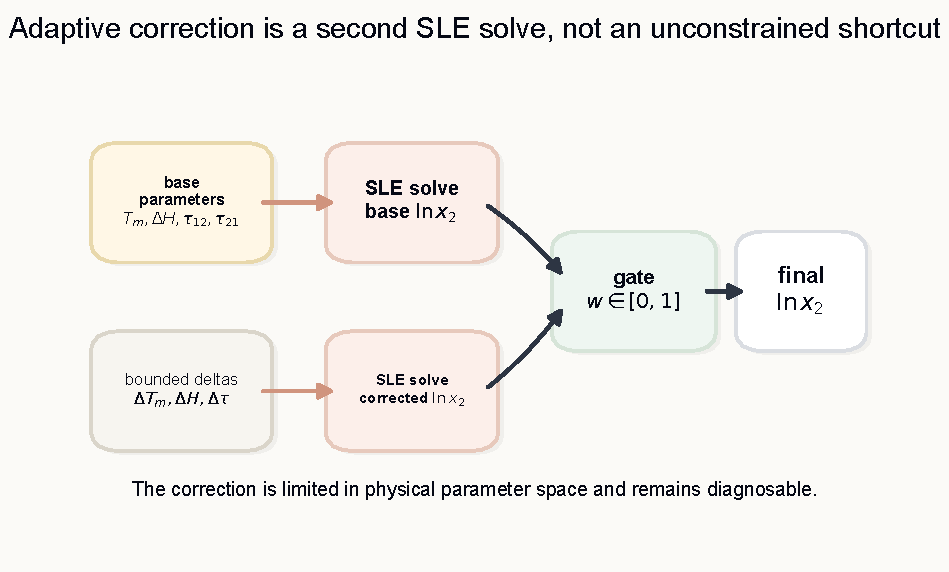
\includegraphics[width=0.86\textwidth]{figures/correction_loop_schematic.pdf}
    \caption{Остаточная коррекция в TGNN-Solv: корректируются физические параметры, затем SLE решается повторно. Это сделано специально, чтобы поправка не разрушала термодинамическую форму модели.}
    \label{fig:correction-loop-appendix}
\end{figure}

\section{Температурные компоненты функции ошибки и случай взрыва vH-local}
\label{app:vh-catastrophe}

Для пары с несколькими температурами естественно требовать, чтобы предсказания были близки к прямой Вант-Гоффа в координатах $q=\ln x_2$ и $u=1/T$. Локальный наклон между двумя соседними точками равен
\begin{equation*}
    s_i=\frac{q_{i+1}-q_i}{u_{i+1}-u_i} .
\end{equation*}
локальный штраф Вант-Гоффа ограничивает изменение этого наклона:
\begin{equation*}
    \mathcal L_{\mathrm{vH-local}}
    =\frac{1}{m-2}\sum_i (s_{i+1}-s_i)^2 .
\end{equation*}
Катастрофа возникает, когда две температуры почти совпадают. Тогда $|u_{i+1}-u_i|$ мало, а градиент по $q_i$ масштабируется как
\begin{equation*}
    \left|\frac{\partial \mathcal L}{\partial q_i}\right|
    =O\!\left(\frac{1}{|u_{i+1}-u_i|^2}\right).
\end{equation*}
Даже небольшой шум измерения или случайная ошибка ранней модели превращается в огромный градиент. Этот сценарий объясняет нестабильные ранние попытки усилить температурную физику.

Стабилизация была сделана в три уровня. Во-первых, включена группировка мини-пакетов по парам: один мини-пакет старается содержать несколько температур для одной и той же пары, иначе температурный компонент функции потерь либо равен нулю, либо строится на случайных сравнениях. Во-вторых, знаменатель $|\Delta(1/T)|$ ограничен снизу:
\begin{equation*}
    \Delta u_{\mathrm{safe}}
    =\operatorname{sign}(\Delta u)\max(|\Delta u|,u_{\min}),
    \qquad u_{\min}=10^{-4}\,\mathrm K^{-1},
\end{equation*}
а вклад одной пары ограничен сверху. В-третьих, компоненты наклона и свободного члена нормируются характерными масштабами, а веса температурных регуляризаторов оставлены малыми.

\begin{figure}[!htbp]
    \centering
    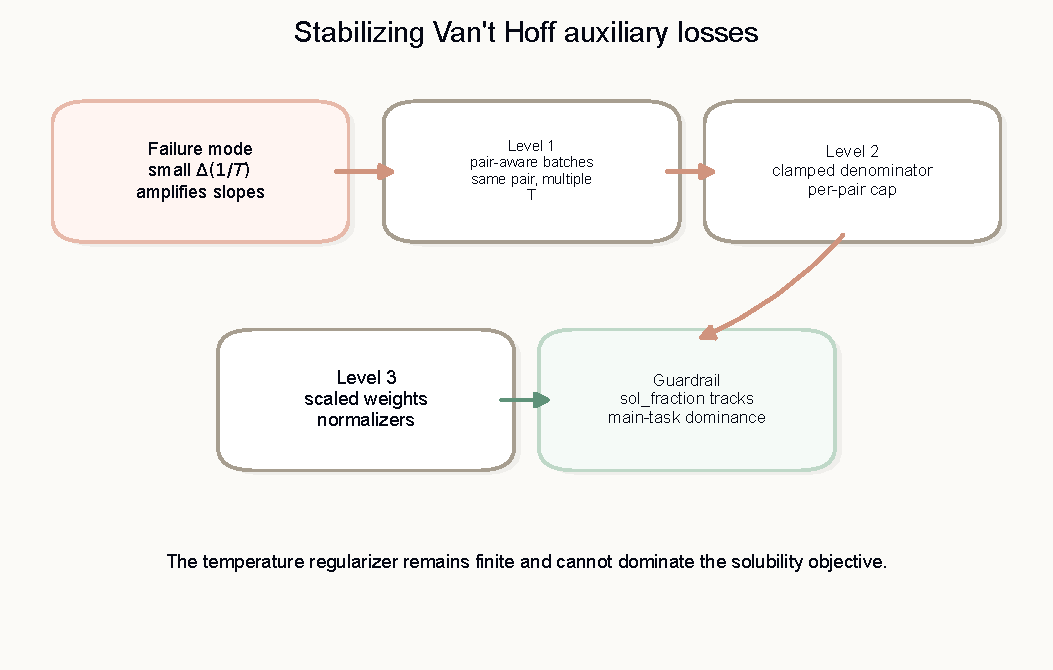
\includegraphics[width=0.96\textwidth]{figures/vh_stability_safeguards.pdf}
    \caption{Стабилизация температурных вспомогательных функций потерь. Главная цель --- не дать температурному регуляризатору вытеснить основной сигнал растворимости.}
    \label{fig:vh-stability-safeguards}
\end{figure}

Главный диагностический ограничитель --- доля ошибки по растворимости в полной функции потерь:
\begin{equation*}
    \mathrm{sol\_fraction}
    =
    \frac{\lambda_{\mathrm{sol}}\mathcal L_{\mathrm{sol}}}
    {\mathcal L_{\mathrm{total}}}.
\end{equation*}
Если эта величина падает ниже $0.1$, обучение фактически перестаёт оптимизировать целевую задачу и начинает подгонять регуляризаторы. Поэтому программа обучения печатает среднее и минимальное значение \code{sol\_fraction} по эпохе и отдельно предупреждает о доминировании регуляризаторов. В тестах для контрастивное выравнивание по параметрам Хансена пути дополнительно проверяется, что при малых весах контрастивная часть не вытесняет основную ошибку по растворимости.

\section{Группировка температурных наблюдений по парам}
\label{app:pair-aware-batching}

Температурные ограничения являются условными: они имеют смысл только внутри одной пары «вещество--растворитель». Если в мини-пакете лежат разные пары, сравнение $q(T_2)-q(T_1)$ смешивает температурный эффект с химическим различием. Поэтому загрузчик данных может группировать строки так, чтобы для части пар в мини-пакете присутствовало несколько температур. Формально цель переходит от независимой построчной регрессии
\begin{equation*}
    \sum_i \ell(f(s_i,v_i,T_i),q_i)
\end{equation*}
к смешанной задаче
\begin{equation*}
    \sum_i \ell_i
    +
    \sum_{(s,v)}
    \Omega\left(\{f(s,v,T_j):T_j\in\mathcal T_{s,v}\}\right),
\end{equation*}
где $\Omega$ задаёт монотонность, локальную линейность или совпадение с наклоном аппроксимации Вант-Гоффа. Это важное изменение протокола: оно делает физический компонент функции потерь наблюдаемым на уровне мини-пакета.

\section{Оптимизация, переобучение и балансировка регуляризации}
\label{app:optimization}

Реализация обучения опирается на PyTorch~\cite{paszke2019}. Основная оптимизация использует AdamW \cite{kingma2015,loshchilov2019}. Для градиента $g_t$ моменты обновляются как
\begin{equation*}
    m_t=\beta_1m_{t-1}+(1-\beta_1)g_t,
    \qquad
    v_t=\beta_2v_{t-1}+(1-\beta_2)g_t^2,
\end{equation*}
после чего применяется раздельное затухание весов:
\begin{equation*}
    \theta_{t+1}
    =\theta_t
    -\eta_t\frac{\hat m_t}{\sqrt{\hat v_t}+\varepsilon}
    -\eta_t\lambda_{\mathrm{wd}}\theta_t .
\end{equation*}
Для физической модели это особенно важно: параметры ветви решателя имеют разные масштабы, а обычный стохастический градиентный спуск плохо переносит смесь $T_m$, $\Delta H_{fus}$, $\tau$ и скрытых векторов. Перед шагом оптимизатора применяется ограничение нормы градиента
\begin{equation*}
    g\leftarrow g\min\left(1,\frac{c}{\|g\|_2}\right),
\end{equation*}
что защищает обучение от редких больших градиентов через решатель и температурные регуляризаторы.

Переобучение в этом проекте проявляется не только как разрыв между обучением и тестом. Для модели с физическими ограничениями есть второй тип переобучения: регуляризаторы могут стать слишком хорошими относительно основной задачи, а MAE по растворимости не улучшится. Поэтому логируются не только полная функция потерь и MAE, но и исходный и взвешенный вклад каждого компонента, \code{sol\_fraction}, максимальное отношение полной ошибки к ошибке по растворимости и число мини-пакетов, где регуляризаторы доминировали. Это инженерная, но необходимая часть математического контроля: многокомпонентная функция ошибки без таких диагностик неинтерпретируема.

\begin{figure}[!htbp]
\centering
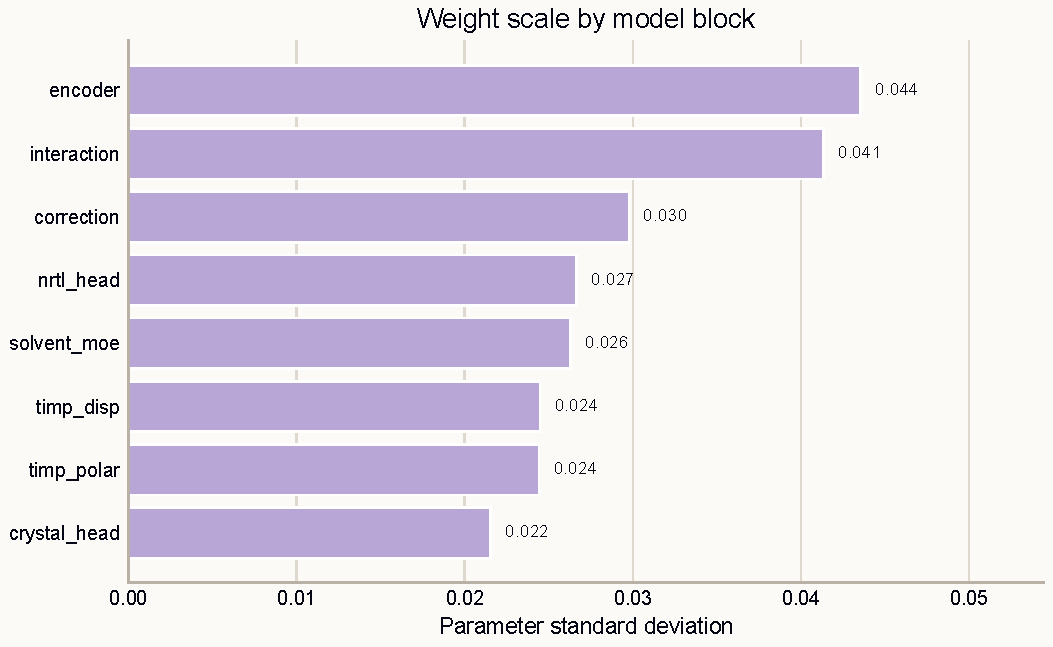
\includegraphics[width=0.86\textwidth]{weight_group_stats.pdf}
\caption{Диагностика масштабов весов по блокам модели. Она используется как грубый контроль того, не «умирает» ли отдельная ветвь и не доминирует ли один блок над остальной архитектурой после добавления новых регуляризаторов.}
\label{fig:weight-group-stats}
\end{figure}

Раннее прекращение обучения во второй и третьей фазах хранит лучшее состояние по валидационной средней абсолютной ошибке и восстанавливает его после остановки. Это важно для TGNN-Solv: поздние эпохи могут улучшать вспомогательные физические величины, но ухудшать целевую растворимость. Критерий остановки привязан к валидационному показателю, а не к сумме всех регуляризаторов.

\section{Гиперпараметрический поиск: Optuna, TPE и раннее отсечение}
\label{app:optuna}

Гиперпараметры подбирались не полным перебором. Пространство содержит категориальные и непрерывные параметры: размер скрытого слоя, число графовых и слоёв внимания, размер парного вектора, вероятность случайного выключения нейронов, шаг обучения, ограничение нормы градиента, режим $\tau(T)$, число экспертов в смеси экспертов, параметры GPS и дескрипторного расширения. Полный перебор по сетке был бы экспоненциально дорогим.

В Optuna стандартный байесовский механизм --- древовидная оценка Парзена (Tree-structured Parzen Estimator) \cite{akiba2019,bergstra2011}. Пусть уже выполнены испытания $(x_i,y_i)$, где $x_i$ --- гиперпараметры, а $y_i$ --- валидационный MAE. По квантилю $y^*$ испытания делятся на лучшие и худшие:
\begin{equation*}
    l(x)=p(x\mid y<y^*),
    \qquad
    g(x)=p(x\mid y\geq y^*).
\end{equation*}
Следующая точка выбирается так, чтобы увеличить отношение
\begin{equation*}
    \frac{l(x)}{g(x)}.
\end{equation*}
Это эквивалентно поиску точки с большой ожидаемой прибылью: гиперпараметры должны быть похожи на хорошие прогоны и непохожи на плохие. Для дорогих запусков может использоваться раннее отсечение неудачных запусков \cite{li2018}: испытание сообщает промежуточные значения, и если его траектория явно хуже уже наблюдавшихся, он останавливается до окончания планового прогона. В текущем коде основной модуль подбора минимизирует валидационный MAE; раннее отсечение не является центральным результатом, но математически совместимо с тем же протоколом.

\begin{figure}[!htbp]
    \centering
    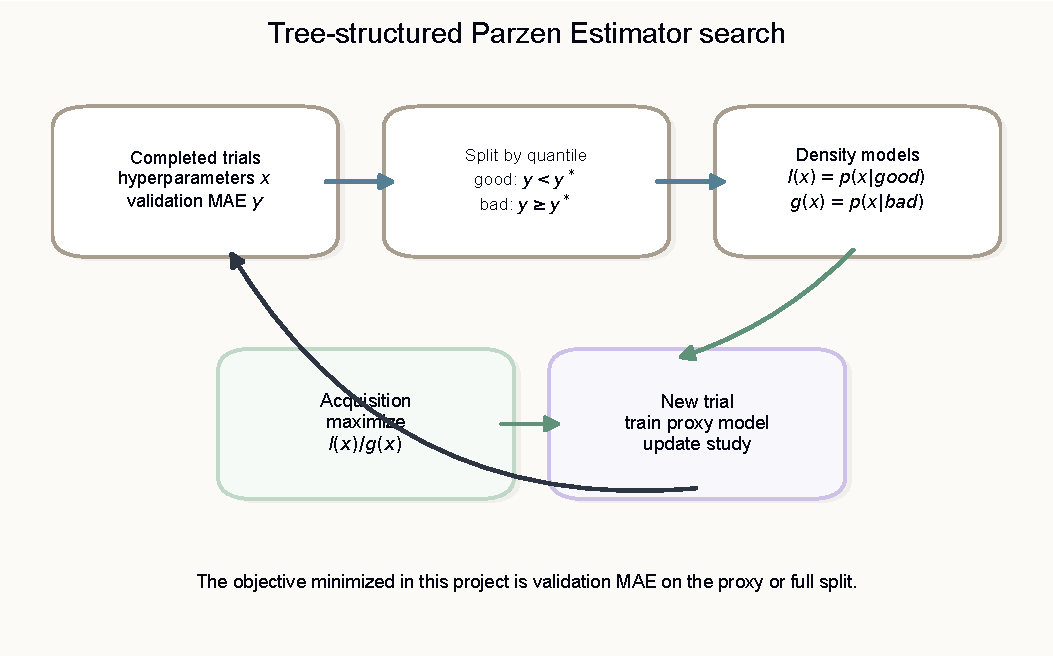
\includegraphics[width=0.96\textwidth]{figures/optuna_tpe_schematic.pdf}
    \caption{Схема TPE-поиска гиперпараметров. В отчёте результаты Optuna используются как источник настроенных конфигураций, а не как самостоятельное доказательство превосходства модели.}
    \label{fig:optuna-tpe-schematic}
\end{figure}

Валидационная выборка в таком протоколе выполняет две роли: по ней выбираются гиперпараметры и по ней же работает раннее прекращение обучения. Поэтому валидационный MAE после поиска является оптимистичной оценкой и не должен использоваться как финальное качество модели. Для вывода нужны тестовая часть, зафиксированный манифест поиска и повторение на нескольких зёрнах.

В приближённом поиске для DirectGNN использовалось $20$ испытаний Optuna на малом каркасном протоколе с базовым бюджетом $4$ эпохи и терпением ранней остановки $2$ эпохи. Для остальных вариантов настройки следует читать как зафиксированные рабочие конфигурации, а не как результат исчерпывающего поиска по всему пространству. Главное практическое следствие остаётся тем же: последующие гипотезы нельзя проверять против слабой случайной конфигурации; сравнение должно идти против настроенного контроля.

\section{Дескрипторное расширение графового представления}
\label{app:descriptor-augmentation}

В проекте проверялся не только «чистый» графовый путь, но и гибридный вариант с RDKit-дескрипторами. Причина практическая: графовый блок может в принципе выучить молекулярную массу, число доноров водородной связи, полярную поверхность и липофильность, но заставлять его каждый раз восстанавливать эти величины из нуля не всегда эффективно. Дескрипторы добавляют известные химические координаты как явные признаки, а графовая часть остаётся ответственной за структуру и контекст взаимодействия.

Пусть $d_s$ и $d_v$ --- нормированные векторы дескрипторов растворяемого вещества и растворителя. Нормировка считается только по обучающей выборке:
\begin{equation*}
    \tilde d=\frac{d-\mu_{\mathrm{train}}}{\sigma_{\mathrm{train}}+\varepsilon}.
\end{equation*}
В парное представление подаются не только сами дескрипторы, но и простые взаимодействия:
\begin{equation*}
    d_{\mathrm{pair}}
    =
    [\tilde d_s,\tilde d_v,\tilde d_s-\tilde d_v,
      |\tilde d_s-\tilde d_v|,\tilde d_s\odot \tilde d_v].
\end{equation*}
После малой проекционной сети этот вектор добавляется к скрытому парному вектору и снова приводится к размерности \code{pair\_dim}. Такой путь не подменяет физическую модель: SLE-решатель, NRTL-блок и кристаллический выходной блок остаются теми же. Он только даёт выходным блокам более доступные химические координаты.

Дескрипторы не решают структурную экстраполяцию автоматически. Они помогают там, где нужное свойство выражается через известные глобальные координаты. Локальные эффекты --- различие положений заместителей, водородно-связанные мотивы и ассоциация растворителя --- всё равно требуют графового или физического представления. Дескрипторные конфигурации рассматриваются как сильные гибридные абляции, а не как замена TGNN-Solv.

\section{Воспроизводимость экспериментов}
\label{app:artifact-contract}

Отдельная инженерная часть проекта --- единая запись эксперимента. Она нужна для того, чтобы результат можно было проверить без устных пояснений. Минимальная запись одного запуска имеет вид
\begin{equation*}
    \mathcal A
    =
    (D_{\mathrm{train}},D_{\mathrm{val}},D_{\mathrm{test}},
     C,s,\theta,M,P,R),
\end{equation*}
где $D$ --- обучающая, валидационная и тестовая части, $C$ --- конфигурация, $s$ --- начальное зерно генератора случайных чисел, $\theta$ --- сохранённое состояние модели, $M$ --- метрики, $P$ --- предсказания, $R$ --- описание запуска с версией кода и окружением. Для научного отчёта важна не служебная организация хранения, а состав записи: разбиение, конфигурация, веса, метрики, предсказания, промежуточные физические величины и описание фильтрации строк.

Такая запись особенно важна для этого проекта, потому что часть отрицательных результатов связана не с архитектурой, а с протоколом: преобразование единиц, добавление IDAC-строк напрямую в SLE-таблицу, изменение валидационной и тестовой частей, сокращённый бюджет вместо полного обучения. Если запуск не содержит разбиений, конфигурации и предсказаний, то нельзя понять, является ли изменение качества научным эффектом или сменой протокола.

\section{Линейная проба как проверка качества представлений}
\label{app:linear-probe}

Линейная проба отвечает на вопрос: насколько химически осмысленная информация уже линейно доступна в замороженном векторном представлении. Пусть $Z\in\mathbb R^{n\times d}$ --- матрица векторных представлений, а $Y\in\mathbb R^{n\times k}$ --- RDKit-дескрипторы или физические свойства. Обучается гребневая регрессия
\begin{equation*}
    W^*=(Z^\top Z+\lambda I)^{-1}Z^\top Y.
\end{equation*}
Если $R^2$ высок на обучающей части, но резко падает на тесте по новым каркасам, представление кодирует свойства только внутри виденных каркасов. Если $R^2$ сохраняется, проблема скорее находится в выходных блоках или физическом ограничительном слое.

В экспериментах TIMP и контрастивного выравнивания по параметрам Хансена этот тест использовался как диагностический, а не как финальная метрика. Он показывает, что канальное выравнивание улучшает доступность физико-химических координат в векторном представлении и уменьшает коллапс дисперсионного и полярного каналов. Это согласуется с гипотезой, что структурная экстраполяция требует не только большего набора данных, но и более переносимого пространства признаков.

При этом TIMP пока не доказал улучшения итоговой растворимости. Более строгая проверка должна разделять две причины неудачи. Если линейная проба даёт высокий $R^2$ на обучающей части и низкий на тестовой, физические каналы переобучаются на виденные каркасы. Если $R^2$ низкий уже на обучении, разделение на дисперсионный и полярный каналы само по себе слишком ограничивает выразительность представления.

\begin{figure}[!htbp]
\centering
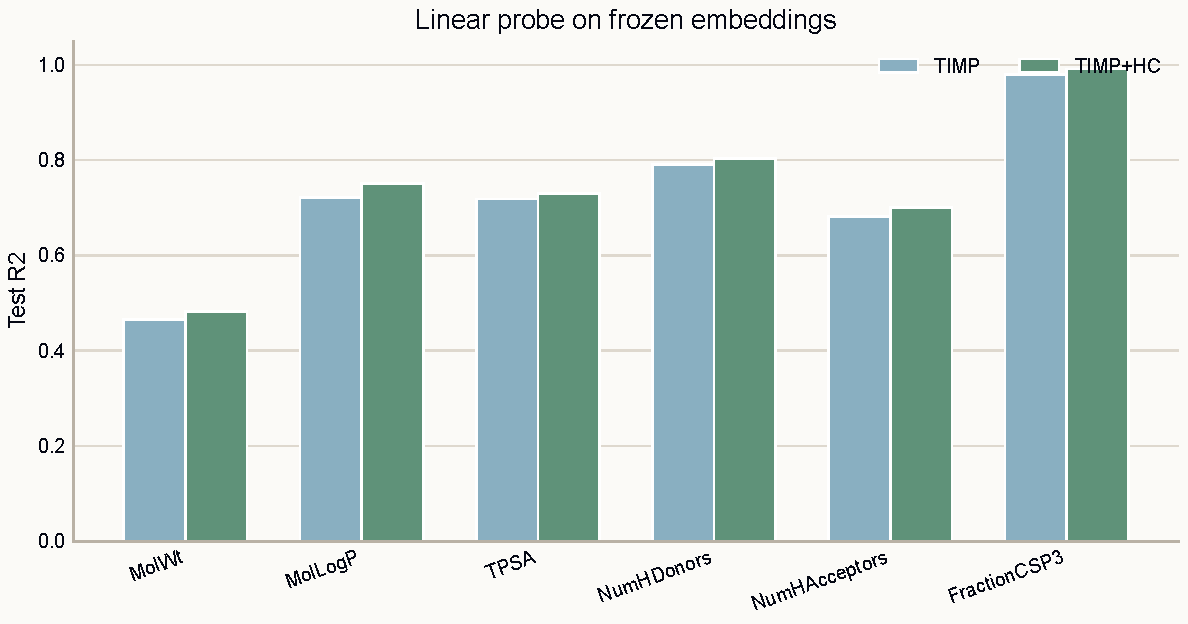
\includegraphics[width=0.88\textwidth]{descriptor_probe_bars.pdf}
\caption{Пример линейной диагностической пробы для TIMP-вариантов. Высокий $R^2$ по простым RDKit-дескрипторам означает, что соответствующая химическая координата линейно доступна в замороженном представлении; низкий $R^2$ указывает, что свойство либо не закодировано, либо закодировано нелинейно.}
\label{fig:descriptor-probe-bars}
\end{figure}

\section{Неопределённость, область применимости и прикладной контур}
\label{app:uncertainty-ood}

Для прикладного использования важно не только среднее предсказание, но и доверие к нему. В реализованном контуре есть два источника эпистемической неопределённости. Первый --- метод Монте-Карло со случайным выключением нейронов \cite{gal2016}: случайное выключение нейронов остаётся активным при применении модели, модель прогоняется $M$ раз, и оцениваются
\begin{equation*}
    \hat\mu=\frac1M\sum_{m=1}^M q_m,
    \qquad
    \hat\sigma^2=\frac1{M-1}\sum_{m=1}^M(q_m-\hat\mu)^2.
\end{equation*}
Второй --- ансамбль независимых моделей, где дисперсия между моделями играет ту же роль \cite{lakshminarayanan2017}. Калибровка проверяется через долю истинных значений внутри интервала $[q_{0.05},q_{0.95}]$:
\begin{equation*}
    \mathrm{PICP}_{90}
    =\frac1n\sum_i
    \mathbb I\{q_i\in[\hat q_{i,0.05},\hat q_{i,0.95}]\}.
\end{equation*}
Хорошо откалиброванная модель должна иметь $\mathrm{PICP}_{90}\approx0.9$ при разумной ширине интервала; сама калибровка вероятностных выходов является отдельной проверкой, а не следствием низкой MAE~\cite{guo2017}.

Область применимости оценивается двумя независимыми признаками. Первый --- расстояние Махаланобиса в пространстве скрытых парных представлений:
\begin{equation*}
    d_M(z)=
    \sqrt{(z-\mu)^\top(\Sigma+\lambda I)^{-1}(z-\mu)}.
\end{equation*}
Порог задаётся процентилем распределения обучающей части. Второй --- ближайшее сходство отпечатков Моргана по Танимото отдельно для вещества и растворителя:
\begin{equation*}
    T(A,B)=\frac{|A\cap B|}{|A\cup B|}.
\end{equation*}
Если расстояние в пространстве скрытых представлений велико и ближайшая химическая схожесть мала, предсказание помечается как находящееся вне области применимости. Такой флаг не предсказывает ошибку напрямую, но запрещает использовать число как обычную оценку внутри области применимости.

\begin{figure}[!htbp]
    \centering
    \includegraphics[width=0.86\textwidth]{figures/uncertainty_ad_schematic.pdf}
    \caption{Контур неопределённости и области применимости. Он нужен для прикладных сценариев: ранжирование растворителей без предупреждения о выходе из области применимости опасно, даже если среднее предсказание выглядит правдоподобно.}
    \label{fig:uncertainty-ad-appendix}
\end{figure}

Прикладные сценарии используют эту же пару величин: среднее предсказание и риск. Для скрининга растворителей можно записать простую функцию полезности
\begin{equation*}
    U(s,T)=\hat q(s,T)-\beta\hat\sigma(s,T)-\eta\,\mathbb I_{\mathrm{OOD}}(s,T)+C(s,T),
\end{equation*}
где $C$ содержит технологические ограничения: температуру, безопасность, стоимость, желательную разницу растворимости между горячей и холодной точкой. Жёсткий индикатор $\mathbb I_{\mathrm{OOD}}$ удобен для предупреждений, но может создавать скачок ранжирования около границы области применимости. Более гладкая прикладная версия должна использовать мягкий штраф, например
\begin{equation*}
    U_{\mathrm{soft}}(s,T)
    =
    \hat q(s,T)-\beta\hat\sigma(s,T)
    -\eta\,\min\!\left(1,\frac{d_M(z)}{d_{\mathrm{thr}}}\right)
    +C(s,T).
\end{equation*}
Прикладной слой не является отдельной моделью. Это способ использовать TGNN-Solv как ранжирующий термодинамический модуль с явным предупреждением о неопределённости.

\section[Количественная мера идентифицируемости физических параметров]{Количественная мера идентифицируемости\\физических параметров}
\label{app:identifiability-quantitative}

Коллинеарность температурной чувствительности параметров $\Delta H_{\mathrm{fus}}$ и NRTL в линейном приближении объясняет, почему растворимость в узком температурном диапазоне содержит мало независимой информации об этих параметрах.

Запишем линеаризованную модель для $n$ наблюдений одной пары при инверсных температурах $u_k = 1/T_k$. В приближении постоянной энтальпии растворения и температурно-линейного NRTL:
\begin{equation}
    \ln x_2(T_k) \approx -\frac{\dHfus}{R} u_k - \beta_{\mathrm{eff}} u_k + c_0,
\end{equation}
где $\beta_{\mathrm{eff}} = \beta_{12} + \beta_{21}$ — эффективный температурный вклад активности. Матрица плана $X \in \mathbb R^{n \times 3}$ для системы из $n$ наблюдений имеет вид
\begin{equation*}
    X = \begin{pmatrix} -u_1 & -u_1 & 1 \\ -u_2 & -u_2 & 1 \\ \vdots & \vdots & \vdots \\ -u_n & -u_n & 1 \end{pmatrix}.
\end{equation*}
Первые два столбца идентичны; $\mathrm{rank}(X) \le 2$, и матрица $X^\top X$ вырождена в точности.

\begin{claim}
В линейном приближении $\dHfus/R$ и $\beta_{\mathrm{eff}}$ абсолютно неразличимы из SLE-наблюдений без дополнительных ограничений (прямых меток $T_m$ или других параметров NRTL).
\end{claim}

Точное совпадение столбцов относится только к этой линейной редукции и к режиму, где температурный вклад NRTL фактически пропорционален $1/T$. В полной нелинейной модели NRTL столбцы чувствительности уже не обязаны быть идентичными. Тогда задача обычно становится не строго вырожденной, а плохо обусловленной: малые изменения данных или начальных условий могут сильно менять разделение между кристаллическим вкладом и активностью. Таблица с числом обусловленности ниже является численной иллюстрацией плохой обусловленности, а не строгим доказательством глобального вырождения.

Нелинейность разделяет эти вклады через разные функциональные формы: $\dHfus$ входит в $\Phi(T) = \dGfus(T)/RT$ через полиномиальную коррекцию с $\Delta C_p$, а NRTL-ветвь имеет другую нелинейную зависимость от температуры.

Для количественной оценки плохой обусловленности задачи используется число обусловленности матрицы Якоби $J$ функции потерь:
\begin{equation}
    \kappa(J^\top J) = \frac{\lambda_{\max}(J^\top J)}{\lambda_{\min}(J^\top J)}.
\end{equation}

\begin{estimate}[Зависимость числа обусловленности от температурного диапазона]
При численном исследовании с $n = 5$ равномерно распределёнными температурами число обусловленности убывает с расширением температурного диапазона:

\begin{table}[!htbp]
\centering
\caption{Число обусловленности матрицы Якоби в зависимости от температурного диапазона.}
\begin{tabularx}{0.6\textwidth}{C{2.2cm}C{2.2cm}C{2.2cm}}
\toprule
Диапазон T & $T_{\max}/T_{\min}$ & $\kappa(J^\top J)$ \\
\midrule
280--310 K & 1.107 & $\sim 200$ \\
280--350 K & 1.250 & $\sim 50$ \\
280--420 K & 1.500 & $\sim 15$ \\
\bottomrule
\end{tabularx}
\end{table}

Широкий температурный диапазон существенно улучшает идентифицируемость физических параметров, а не только проверяет точность предсказания.
\end{estimate}

\section{Информационное содержание SLE и IDAC данных}
\label{app:idac-information}

\begin{claim}
Добавление IDAC-строки в SLE-таблицу некорректно, потому что при $x_2 \to 0$ SLE-решение имеет вид
$$\ln x_2 \approx -\Phi(T) - \ln\gamma_2^\infty,$$
что не является измеренной растворимостью (в частности, при $T \ll T_m$ величина $\Phi(T) \to +\infty$). Корректная постановка --- отдельная функция ошибки на $\ln\gamma_2^\infty$, не проходящая через физический решатель.
\end{claim}

Каждая IDAC-точка при температуре $T$ ограничивает параметры NRTL через уравнение:
\begin{equation*}
    \ln\gamma_2^\infty = \tau_{12}(T) + \tau_{21}(T) \exp(-\alpha \tau_{21}(T)).
\end{equation*}
При наличии нескольких температур с режимом $\code{ref\_invT}$:
\begin{equation}
    \tau_{ij}(T)=\tau_{ij}^{\mathrm{ref}}
    +\beta_{ij}\left(\frac{1}{T}-\frac{1}{T_{\mathrm{ref}}}\right),
\end{equation}
каждая дополнительная температура ужесточает определение пары $(\tau_{ij}^{\mathrm{ref}}, \beta_{ij})$.

Оценка ранга ниже является верхней границей в идеализированной локальной модели. Она не гарантирует, что реальный численный ранг будет достигнут: симметричные параметры, близкие температуры и слабая температурная зависимость могут снова сделать столбцы чувствительности почти коллинеарными.

\begin{estimate}[Ранг совместной задачи]
SLE при $n_S$ температурах одной пары даёт ранг не более $2$ по параметрам $(\dHfus/R, \beta_{\mathrm{eff}}, c_0)$. IDAC при $n_I$ температурах той же пары напрямую ограничивает $(\tau_{12}^{\mathrm{ref}}, \beta_{12})$ и аналогично $(\tau_{21}^{\mathrm{ref}}, \beta_{21})$, что даёт ранг не более $2$ в одной паре переменных. Совместная задача имеет ранг, не превышающий $4$ в этом упрощённом описании, и достигает этого ранга только при достаточно разнесённых температурах и линейно независимых столбцах чувствительности. При типичных близких температурах или симметричных значениях $\tau$ реальный численный ранг может быть ниже.
\end{estimate}

\section[Скорость сходимости градиентного обучения через физический решатель]{Скорость сходимости градиентного обучения\\через физический решатель}
\label{app:convergence}

Сравним скорость сходимости градиентного обучения для TGNN-Solv и DirectGNN. Для DirectGNN градиент прямого предсказания:
\begin{equation}
    \nabla_\theta \mathcal L_{\mathrm{Direct}} = \frac{1}{n}\sum_i \rho'_i \cdot \nabla_\theta f_\theta(x_i),
\end{equation}
где норма $\|\nabla_\theta f_\theta\|$ определяется архитектурой сети и не зависит от физической области.

Для TGNN-Solv дополнительный множитель --- производная через SLE-решатель (раздел~\ref{app:implicit}):
\begin{equation}
    \frac{\partial \ln x_2^*}{\partial \tau_{ij}} = -\frac{\partial \ln\gamma_2/\partial\tau_{ij}}{1 + x_2^* \eta},
    \quad
    \eta = \frac{\partial\ln\gamma_2}{\partial x_2}.
\end{equation}

\begin{estimate}[Нестабильность градиента при некоторых значениях $x_2$]
При $x_2^* \eta \approx -0.9$ знаменатель равен $0.1$, и градиент через решатель усиливается в $10$ раз относительно DirectGNN. Это создаёт нестабильность на ранних эпохах, когда NRTL-параметры инициализированы случайно и $\eta$ неконтролируем.
\end{estimate}

Эта оценка показывает возможный механизм нестабильности, но сама по себе не говорит, как часто режим $x_2^*\eta\approx-0.9$ встречается в корпусе. Для строгого эмпирического вывода нужно логировать распределение знаменателя $1+x_2^*\eta$ по эпохам и долю строк ниже заданных порогов. Трёхфазная схема обучения уменьшает риск: в фазе~1 основная ветвь NRTL не получает градиента от SLE, и знаменатель может стабилизироваться до включения этого пути в фазе~2. Проблема при этом не исчезает полностью: при включении SLE-пути нестабильные параметры всё равно возможны. Фазовое обучение является защитной эвристикой, а не заменой численного аудита градиентов.

\section{Гладкость решения SLE по параметрам}
\label{app:smoothness-implicit}

\begin{claim}[Локальная гладкость]
Если в найденном решении выполнено
\begin{equation*}
    1+x_2^*\eta \ne 0,
    \qquad
    \eta=\frac{\partial \ln\gamma_2}{\partial x_2},
\end{equation*}
то в окрестности рассматриваемых параметров решение SLE гладко зависит от $\tau_{12},\tau_{21},\alpha,T_m,\dHfus$, и неявное дифференцирование корректно.
\end{claim}

\begin{proof}[Локальный аргумент]
Это прямое применение теоремы о неявной функции к невязке SLE $F(x_2,\theta)=0$. Условие применимости --- ненулевая производная $\partial F/\partial x_2$, которая в используемой записи пропорциональна $1+x_2^*\eta$.
\end{proof}

Ограничения $|\tau_{ij}|\le\tau_{\max}$, $\alpha\in[0.1,0.6]$, ограничение $x_2\in[\varepsilon,1-\varepsilon]$ и нижнее ограничение знаменателя в коде являются численными защитными условиями, а не самостоятельным аналитическим доказательством глобальной гладкости. Чтобы утверждать запас строго, нужно либо вывести явную верхнюю оценку $C(\tau_{\max},\alpha)$ для $|x_2\eta|$, либо приложить отдельный сеточный аудит минимального значения $|1+x_2\eta|$ на допустимой области. В отчёте используется более осторожная формулировка: ограничения диапазонов $\tau$ нужны одновременно для химической разумности и для защиты корректности обратного распространения.

\section{Условия значимости теплоёмкостной поправки}
\label{app:dcp-significance}

Обозначим редуцированную температуру $\tau_r = T/T_m$. Теплоёмкостная поправка записывается как:
\begin{equation}
    \mathrm{corr}(\tau_r) = \frac{\dCpfus}{R} \, B(\tau_r),
    \quad
    B(\tau_r) = \frac{1-\tau_r}{\tau_r} + \ln\tau_r.
\end{equation}
Функция $B(\tau_r)$ монотонно убывает при $\tau_r \to 1$ и обращается в ноль в точке плавления. Производная
\begin{equation*}
    B'(\tau_r)=-\frac{1}{\tau_r^2}+\frac{1}{\tau_r}
    =\frac{\tau_r-1}{\tau_r^2}<0
\end{equation*}
при $\tau_r < 1$.

\begin{estimate}[Условие значимости поправки]
При $\dCpfus = 40\,\mathrm{J\,mol^{-1}K^{-1}}$ и $T = 298\,\mathrm K$ поправка превышает $0.5$ в $\ln x_2$ при $T_m > 415\,\mathrm K$. Это иллюстративное значение: теплоёмкостные и энтропийно-энтальпийные параметры органических твёрдых веществ существенно меняются с размером молекулы, гибкостью и типом фазового перехода~\cite{yalkowsky1979,acree2010}. Для малых органических молекул порядок $\Delta C_p^{\mathrm{fus}}$ может отличаться в несколько раз, так что порог $415\,\mathrm K$ не является универсальной границей. При $T_m = 550\,\mathrm K$ и выбранном $\dCpfus$ поправка составляет $1.6$. Если $\dCpfus$ в два раза меньше, пороговый эффект уменьшается в два раза; если больше --- растёт пропорционально. Для высокоплавких соединений, прежде всего жёстких и ароматических молекул с заметной теплоёмкостной разницей, приближение $\dCpfus = 0$ может быть существенным источником систематической ошибки.
\end{estimate}

Это объясняет наблюдаемую корреляцию ошибок с молекулярной массой и ароматичностью в тестовом наборе: более тяжёлые молекулы (с большим $T_m$) несут большую систематическую ошибку при $\dCpfus = 0$.

Но обучаемая теплоёмкостная поправка не должна вводиться без контроля. В текущих данных практически нет прямых меток $\dCpfus$, поэтому модель может предсказывать этот параметр только из косвенной ошибки растворимости и слабых структурных закономерностей. Если типичная ошибка $\dCpfus$ составляет десятки $\mathrm{J\,mol^{-1}K^{-1}}$, шум от поправки может быть сопоставим с самой поправкой. Значит, полезность $\dCpfus$-ветви нужно проверять отдельной абляцией, а не считать следствием более полной термодинамической формулы.

\section{Граница Крамера-Рао для идентификации NRTL-параметров}
\label{app:cramer-rao}

Граница Крамера-Рао даёт идеализированную нижнюю оценку неопределённости параметров при заданной модели шума. Это ориентир, а не эмпирическое обещание качества: ниже этой дисперсии несмещённая оценка не может опуститься при правильно специфицированной модели.

Пусть для одной пары есть $n$ независимых IDAC-измерений $\ln\gamma^\infty$ при температурах $T_1, \ldots, T_n$ с шумом $\sigma$. Здесь предполагаются независимые измерения, несмещённая оценка, корректная дифференцируемая модель и известная однородная дисперсия шума. Если экспериментальная ошибка систематически зависит от метода измерения или источника, то такая граница остаётся полезной нижней оценкой, но уже не описывает реальную неопределённость полностью. Параметры: $\theta = (\tau_{12}^{\mathrm{ref}}, \beta_{12}, \tau_{21}^{\mathrm{ref}}, \beta_{21})$. Матрица Фишера:
\begin{equation}
    \mathcal{I}(\theta)_{ij} = \frac{1}{\sigma^2} \sum_{k=1}^n \frac{\partial \ln\gamma^\infty(T_k)}{\partial \theta_i} \cdot \frac{\partial \ln\gamma^\infty(T_k)}{\partial \theta_j}.
\end{equation}
По теореме Крамера-Рао дисперсия несмещённой оценки ограничена снизу:
\begin{equation}
    \mathrm{Var}(\hat{\theta}_i) \ge [\mathcal{I}(\theta)^{-1}]_{ii}.
\end{equation}

\begin{estimate}[Минимальное число IDAC-точек]
Для одного эффективного параметра при $\sigma = 0.2$ в $\ln\gamma^\infty$ и типичной производной порядка $0.8$ одна IDAC-точка даёт
\begin{equation*}
    \mathcal I = \frac{0.8^2}{0.2^2}=16,
    \qquad
    \mathrm{SD}(\hat\tau)\ge\frac{1}{\sqrt{16}}=0.25.
\end{equation*}
Это число корректно только в одномерной редукции, где остальные параметры зафиксированы или уже известны. Для полной NRTL-пары одна IDAC-точка даёт один скалярный градиент по нескольким параметрам; матрица Фишера имеет ранг не выше $1$ и не идентифицирует одновременно $\tau_{12}$, $\tau_{21}$ и $\alpha$ (или температурные коэффициенты $\beta_{ij}$). При $n = 5$ независимых температурах в одномерной редукции нижняя граница падает до $0.11$, но в полной модели нужен ещё и численный ранг матрицы чувствительности.

Расширение IDAC-корпуса с 404 до 14 900 строк является важным источником информации о форме ветви активности. Однако точное пересечение с SLE-парами равно нулю, и эти строки не идентифицируют NRTL-параметры тестовых SLE-пар напрямую. Их роль слабее и честнее: они обучают переносимое представление активности и уменьшают неопределённость NRTL-ветви на химически похожих парах. Это допущение переноса должно проверяться абляцией «с IDAC / без IDAC» на одних и тех же SLE-разбиениях.
\end{estimate}

\section{Пределы применимости}
\label{app:limits}

Модель рассчитана на молекулярные органические системы, где растворимость можно описывать через бинарное SLE и эффективный коэффициент активности. За пределами этой постановки результаты нужно считать эвристическими. К таким случаям относятся электролиты и соли, сильная ионизация и pH-зависимость, гидраты и сольваты, полиморфные переходы, реакция вещества с растворителем, многокомпонентные смеси, явная кристаллизация другого твёрдого состояния и системы, где водородно-связанная сетка растворителя требует отдельной ассоциативной модели.

Ограничение также есть у данных. Разбиение по молекулярным каркасам проверяет новые каркасы, но не гарантирует равномерного покрытия химического пространства. Если тестовая молекула содержит функциональные группы, которых нет в обучении и которые не покрыты априорными оценками, физическая формула не восстановит $\tau_{12},\tau_{21}$ без информации о новой химии.

\begin{thebibliography}{99}
\addcontentsline{toc}{section}{Список литературы и источников}

\bibitem{krasnov2025} Krasnov, L., Malikov, D., Kiseleva, M., Tatarin, S., Sosnin, S., Bezzubov, S. BigSolDB 2.0, dataset of solubility values for organic compounds in different solvents at various temperatures. \textit{Scientific Data}, 2025. \url{https://doi.org/10.1038/s41597-025-05559-8}

\bibitem{bigsoldb2026} BigSolDB 2.1: A Comprehensive Dataset of Solubility Values for Organic Compounds in Organic Solvents and Water at Various Temperatures. Zenodo data snapshot used in this work, 2026. \url{https://zenodo.org/records/15094979}

\bibitem{kumoro2010} Kumoro, A. C., Retnowati, D. S., Budiyati, C. S. Solubility of Delphinidin in Water and Various Organic Solvents between (298.15 and 343.15) K. \textit{Journal of Chemical \& Engineering Data}, 55(7), 2603--2606, 2010. \url{https://doi.org/10.1021/je900851k}

\bibitem{prausnitz1998} Prausnitz, J. M., Lichtenthaler, R. N., de Azevedo, E. G. \textit{Molecular Thermodynamics of Fluid-Phase Equilibria}. 3rd ed. Prentice Hall, 1998.

\bibitem{hildebrand1970} Hildebrand, J. H., Prausnitz, J. M., Scott, R. L. \textit{Regular and Related Solutions}. Van Nostrand Reinhold, 1970.

\bibitem{yalkowsky1979} Yalkowsky, S. H. Estimation of entropies of fusion of organic compounds. \textit{Industrial \& Engineering Chemistry Process Design and Development}, 18(1), 108--111, 1979. \url{https://doi.org/10.1021/i260069a021}

\bibitem{acree2010} Acree, W. E., Chickos, J. S. Phase change enthalpies and entropies of organic solids. \textit{Journal of Physical and Chemical Reference Data}, 39(4), 043101, 2010. \url{https://doi.org/10.1063/1.3501239}

\bibitem{joback1987} Joback, K. G., Reid, R. C. Estimation of pure-component properties from group-contributions. \textit{Chemical Engineering Communications}, 57(1--6), 233--243, 1987. \url{https://doi.org/10.1080/00986448708960487}

\bibitem{marrero2001} Marrero, J., Gani, R. Group-contribution based estimation of pure component properties. \textit{Fluid Phase Equilibria}, 183--184, 183--208, 2001. \url{https://doi.org/10.1016/S0378-3812(01)00431-9}

\bibitem{renon1968} Renon, H., Prausnitz, J. M. Local compositions in thermodynamic excess functions for liquid mixtures. \textit{AIChE Journal}, 14(1), 135--144, 1968. \url{https://doi.org/10.1002/aic.690140124}

\bibitem{wilson1964} Wilson, G. M. Vapor-liquid equilibrium. XI. A new expression for the excess free energy of mixing. \textit{Journal of the American Chemical Society}, 86(2), 127--130, 1964. \url{https://doi.org/10.1021/ja01056a002}

\bibitem{abrams1975} Abrams, D. S., Prausnitz, J. M. Statistical thermodynamics of liquid mixtures: a new expression for the excess Gibbs energy of partly or completely miscible systems. \textit{AIChE Journal}, 21(1), 116--128, 1975. \url{https://doi.org/10.1002/aic.690210115}

\bibitem{fredenslund1975} Fredenslund, A., Jones, R. L., Prausnitz, J. M. Group-contribution estimation of activity coefficients in nonideal liquid mixtures. \textit{AIChE Journal}, 21(6), 1086--1099, 1975. \url{https://doi.org/10.1002/aic.690210607}

\bibitem{weidlich1987} Weidlich, U., Gmehling, J. A modified UNIFAC model. 1. Prediction of VLE, hE, and gamma-infinity. \textit{Industrial \& Engineering Chemistry Research}, 26(7), 1372--1381, 1987. \url{https://doi.org/10.1021/ie00067a018}

\bibitem{hansen2007} Hansen, C. M. \textit{Hansen Solubility Parameters: A User's Handbook}. 2nd ed. CRC Press, 2007.

\bibitem{apelblat1999} Apelblat, A., Manzurola, E. Solubilities of salicylic-acid derivatives and p-toluic acid in water from T=(278 to 348) K. \textit{Journal of Chemical Thermodynamics}, 31(1), 85--91, 1999. \url{https://doi.org/10.1006/jcht.1998.0425}

\bibitem{idac_zenodo} TGNN-Solv External IDAC Starter Corpus. Project Zenodo deposit, 2026. \url{https://zenodo.org/records/19484205}

\bibitem{frenkel2006} Frenkel, M., Chirico, R. D., Diky, V., et al. XML-Based IUPAC Standard for Experimental, Predicted, and Critically Evaluated Thermodynamic Property Data Storage and Capture (ThermoML). \textit{Pure and Applied Chemistry}, 78(3), 541--612, 2006. \url{https://doi.org/10.1351/pac200678030541}

\bibitem{nist_thermoml} National Institute of Standards and Technology. ThermoML Archive. \url{https://www.nist.gov/mml/acmd/trc/thermoml/thermoml-archive}

\bibitem{nist_webbook} National Institute of Standards and Technology. NIST Chemistry WebBook, SRD 69. \url{https://webbook.nist.gov/chemistry/}

\bibitem{chemeo} Cheméo. Chemical and physical property database used as a low-confidence auxiliary source for missing phase-change estimates. \url{https://www.chemeo.com/}

\bibitem{landrum2024} Landrum, G. RDKit: Open-source cheminformatics software, 2024. \url{https://www.rdkit.org}

\bibitem{gilmer2017} Gilmer, J., Schoenholz, S. S., Riley, P. F., Vinyals, O., Dahl, G. E. Neural message passing for quantum chemistry. \textit{Proceedings of ICML}, 2017. \url{https://proceedings.mlr.press/v70/gilmer17a.html}

\bibitem{velickovic2018} Veličković, P., Cucurull, G., Casanova, A., Romero, A., Liò, P., Bengio, Y. Graph attention networks. \textit{Proceedings of ICLR}, 2018. \url{https://arxiv.org/abs/1710.10903}

\bibitem{vaswani2017} Vaswani, A., Shazeer, N., Parmar, N., et al. Attention is all you need. \textit{Advances in Neural Information Processing Systems}, 2017. \url{https://arxiv.org/abs/1706.03762}

\bibitem{rampasek2022} Rampášek, L., Galkin, M., Dwivedi, V. P., Luu, A. T., Wolf, G., Beaini, D. Recipe for a general, powerful, scalable graph transformer. \textit{Advances in Neural Information Processing Systems}, 2022. \url{https://arxiv.org/abs/2205.12454}

\bibitem{schutt2018} Schütt, K. T., Sauceda, H. E., Kindermans, P.-J., Tkatchenko, A., Müller, K.-R. SchNet: A deep learning architecture for molecules and materials. \textit{Journal of Chemical Physics}, 148(24), 241722, 2018. \url{https://doi.org/10.1063/1.5019779}

\bibitem{gasteiger2020} Gasteiger, J., Giri, S., Margraf, J. T., Günnemann, S. Directional message passing for molecular graphs. \textit{Proceedings of ICLR}, 2020. \url{https://arxiv.org/abs/2003.03123}

\bibitem{yang2019} Yang, K., Swanson, K., Jin, W., et al. Analyzing learned molecular representations for property prediction. \textit{Journal of Chemical Information and Modeling}, 59(8), 3370--3388, 2019. \url{https://doi.org/10.1021/acs.jcim.9b00237}

\bibitem{rogers2010} Rogers, D., Hahn, M. Extended-connectivity fingerprints. \textit{Journal of Chemical Information and Modeling}, 50(5), 742--754, 2010. \url{https://doi.org/10.1021/ci100050t}

\bibitem{lusci2013} Lusci, A., Pollastri, G., Baldi, P. Deep architectures and deep learning in chemoinformatics: the prediction of aqueous solubility. \textit{Journal of Chemical Information and Modeling}, 53(7), 1563--1575, 2013. \url{https://doi.org/10.1021/ci400187y}

\bibitem{francoeur2021} Francoeur, P. G., Koes, D. R. SolTranNet: A machine learning tool for fast aqueous solubility prediction. \textit{Journal of Chemical Information and Modeling}, 61(6), 2530--2536, 2021. \url{https://doi.org/10.1021/acs.jcim.1c00331}

\bibitem{boobier2017} Boobier, S., Hose, D. R. J., Blacker, A. J., Nguyen, B. N. Machine learning with physicochemical relationships: solubility prediction in organic solvents and water. \textit{Nature Communications}, 8, 1600, 2017. \url{https://doi.org/10.1038/s41467-017-01920-0}

\bibitem{vermeire2022} Vermeire, F. H., Chung, Y., Green, W. H. Predicting solubility limits of organic solutes for a wide range of solvents and temperatures. \textit{Journal of the American Chemical Society}, 144(24), 10785--10797, 2022. \url{https://doi.org/10.1021/jacs.2c01768}

\bibitem{fastsolv2025} Attia, L., Burns, J. W., Doyle, P. S., et al. Data-driven organic solubility prediction at the limit of aleatoric uncertainty. \textit{Nature Communications}, 16, 7497, 2025. \url{https://doi.org/10.1038/s41467-025-62717-7}

\bibitem{wu2018} Wu, Z., Ramsundar, B., Feinberg, E. N., et al. MoleculeNet: A benchmark for molecular machine learning. \textit{Chemical Science}, 9, 513--530, 2018. \url{https://doi.org/10.1039/C7SC02664A}

\bibitem{raissi2019} Raissi, M., Perdikaris, P., Karniadakis, G. E. Physics-informed neural networks: A deep learning framework for solving forward and inverse problems involving nonlinear partial differential equations. \textit{Journal of Computational Physics}, 378, 686--707, 2019. \url{https://doi.org/10.1016/j.jcp.2018.10.046}

\bibitem{gould2021} Gould, S., Hartley, R., Campbell, D. Deep declarative networks: A new hope. \textit{IEEE TPAMI}, 44(8), 3899--3910, 2021. \url{https://doi.org/10.1109/TPAMI.2021.3055292}

\bibitem{gal2016} Gal, Y., Ghahramani, Z. Dropout as a Bayesian approximation: Representing model uncertainty in deep learning. \textit{Proceedings of ICML}, 2016. \url{https://proceedings.mlr.press/v48/gal16.html}

\bibitem{lakshminarayanan2017} Lakshminarayanan, B., Pritzel, A., Blundell, C. Simple and scalable predictive uncertainty estimation using deep ensembles. \textit{Advances in Neural Information Processing Systems}, 2017. \url{https://papers.nips.cc/paper/2017/hash/9ef2ed4b7fd2c810847ffa85bce38f3c-Abstract.html}

\bibitem{guo2017} Guo, C., Pleiss, G., Sun, Y., Weinberger, K. Q. On calibration of modern neural networks. \textit{Proceedings of ICML}, 2017. \url{https://proceedings.mlr.press/v70/guo17a.html}

\bibitem{paszke2019} Paszke, A., Gross, S., Massa, F., et al. PyTorch: An imperative style, high-performance deep learning library. \textit{Advances in Neural Information Processing Systems}, 2019. \url{https://proceedings.neurips.cc/paper/2019/hash/bdbca288fee7f92f2bfa9f7012727740-Abstract.html}

\bibitem{kingma2015} Kingma, D. P., Ba, J. Adam: A method for stochastic optimization. \textit{Proceedings of ICLR}, 2015. \url{https://arxiv.org/abs/1412.6980}

\bibitem{loshchilov2019} Loshchilov, I., Hutter, F. Decoupled weight decay regularization. \textit{Proceedings of ICLR}, 2019. \url{https://arxiv.org/abs/1711.05101}

\bibitem{huber1964} Huber, P. J. Robust estimation of a location parameter. \textit{Annals of Mathematical Statistics}, 35(1), 73--101, 1964. \url{https://doi.org/10.1214/aoms/1177703732}

\bibitem{akiba2019} Akiba, T., Sano, S., Yanase, T., Ohta, T., Koyama, M. Optuna: A next-generation hyperparameter optimization framework. \textit{Proceedings of KDD}, 2019. \url{https://doi.org/10.1145/3292500.3330701}

\bibitem{bergstra2011} Bergstra, J., Bardenet, R., Bengio, Y., Kégl, B. Algorithms for hyper-parameter optimization. \textit{Advances in Neural Information Processing Systems}, 2011. \url{https://papers.nips.cc/paper/4443-algorithms-for-hyper-parameter-optimization}

\bibitem{li2018} Li, L., Jamieson, K., DeSalvo, G., Rostamizadeh, A., Talwalkar, A. Hyperband: A novel bandit-based approach to hyperparameter optimization. \textit{Journal of Machine Learning Research}, 18(185), 1--52, 2018. \url{https://jmlr.org/papers/v18/16-558.html}


\end{thebibliography}

\end{document}
